\documentclass[11pt,dutch,faculty=we,layout=titlefont,underline=false,titleUppercase=true,titleUnderline=true,numbers=noenddot,twoside,headings=openright]{ugent2016-report}
\usepackage[dutch]{babel}
\usepackage{fontspec,unicode-math}
\usepackage{amsmath}
\usepackage{subcaption}
\usepackage{csquotes}
\usepackage{subfloat}
\usepackage{float}
\usepackage[outputdir=../out]{minted}
\usepackage{enumitem}
\usepackage{afterpage}
\newcommand\blankpage{%
    \null
    \thispagestyle{empty}%
    \newpage}
\raggedbottom

\usepackage{booktabs,makecell}
% Figures
%---------
\usepackage{graphicx, ugent2016-assets}
\graphicspath{{./figures/}}
\usepackage[inkscapelatex=false]{svg}
\usepackage{footmisc}
\usepackage{siunitx}
\usepackage{setspace}
\usepackage{pdfpages}


% Bibliography settings
%-----------------------
\usepackage{tikz}
\usepackage{biblatex}
\addbibresource{bibliography.bib}

\usepackage[hyperfootnotes=true]{hyperref}
\hypersetup{
    colorlinks,
    linkcolor={black},
    citecolor={blue!50!black},
    urlcolor={blue!80!black}
}
\definecolor{lightgrey}{HTML}{AAAAAA}
\setlength{\parindent}{0em}
\renewcommand{\listingscaption}{Codefragment} % Listing->Codeblock


\author{Bram Devlaminck}
\title{Snelle semi-exacte matching\newline van peptiden met een geheugenefficiënte index voor UniProtKB}
%\subtitle{Hello}
\academicyear{2023--2024}
\programme{Informatica}
\studentnumber{01902993}
\email{bram.devlaminck@ugent.be}

\titletext{%
    Promotoren: prof.~dr.~Peter Dawyndt, prof. dr.~ir.~Bart Mesuere \\%
    Begeleiders: dr.~Pieter Verschaffelt, Tibo Vande Moortele
    \\ \\%
    {\small Masterproef ingediend tot het behalen van de academische graad van\\%
    Master of Science in de Informatica%
    }%
}

\babelhyphenation[dutch]{Uni-Prot-KB}


\begin{document}

    \maketitle


    \setmonofont[Scale=MatchLowercase,Contextuals={Alternate}]{Jetbrains Mono}
    \pagenumbering{roman}
    \chapter*{Samenvatting}
Eiwitten zijn alomtegenwoordig en spelen een belangrijke rol in ons dagelijkse leven.
Ze garanderen een correcte werking van belangrijke processen binnen elk organisme.
Hieronder vallen de levensprocessen van ons eigen lichaam, maar ook die van dieren, planten, bacteriën en zelfs virussen.
Deze belangrijke eigenschappen van eiwitten verklaren het bestaan van gespecialiseerde databanken zoals UniProtKB, die voor miljoenen eiwitten bijhouden door welke organismen ze geproduceerd kunnen worden en voor welke functies ze kunnen instaan.
Gebruikmakende van deze databanken probeert men voor eiwitstalen te achterhalen welke organismen aanwezig zijn in een ecosysteem en wat ze doen.
Er is echter een extra stap nodig.
De toestellen die eiwitten inlezen (massaspectrometers), zodat ze later omgezet kunnen worden naar een tekstueel formaat, kunnen dit slechts voor korte fragmenten, ook wel peptiden genoemd.
Daarom worden eerst proteases (eiwitafbrekende enzymen) aan een staal toegevoegd.
Deze zullen de eiwitten ``knippen'', waarna we peptiden bekomen.
\\ \\
Omdat alle eiwitten in een dataset verknipt zijn in peptiden, is er geen zekerheid meer over welke eiwitten er exact aanwezig zijn.
Hier komen tools zoals Unipept van pas om te zoeken uit welke mogelijke eiwitten een peptide afkomstig kan zijn.
Op basis van de gevonden eiwitten kan daarna afgeleid worden welke organismen mogelijks aanwezig zijn, en wat er op dat moment gebeurt in het staal.
De precisie van deze conclusie varieert van peptide tot peptide.
Sommige peptiden bestaan uit een uniek patroon, waardoor ze slechts één mogelijk eiwit kunnen komen.
Andere peptiden komen dan weer erg veel voor, waardoor ze deel uitmaken van duizenden eiwitten.
\\ \\
Zoals eerder vermeld, is Unipept één van de tools die onderzoekers kan helpen bij het vinden van de eiwitten waarvan een peptide onderdeel is.
Bijkomend geeft Unipept ook informatie over welke organismen die eiwitten kunnen produceren en welke functies ze mogelijks uitvoeren.
Unipept heeft op dit moment echter één grote beperking.
Enkel peptiden die ontstaan zijn na het knippen van de eiwitten door de protease trypsine kunnen verwerkt worden.
Dit was tot nu toe geen grote beperking omdat trypsine in de praktijk veruit de meest gebruikte protease is.
Daar komt echter stilaan verandering in.
Daarom is ons doel is om Unipept breder toepasbaar te maken, bijvoorbeeld voor HLA-peptiden.
Deze spelen een belangrijke rol in onderzoek naar kankervaccins.
Het wegwerken van deze beperking, waardoor alle soorten peptiden verwerkt kunnen worden, is de hoofdfocus van deze masterproef.
\\ \\
Om efficiënt alle eiwitten van UniProtKB te doorzoeken, maakt onze oplossing gebruik van een \textit{suffix array}.
Deze datastructuur bestaat uit één lijst die de startpositie van elke mogelijke suffix van alle eiwitten voorstelt.
Een suffix van een woord is een deel van het woord, waarbij de eerste (0 of meerdere) tekens overgeslagen worden.
Het eiwit \texttt{ACGT} heeft bijvoorbeeld vier verschillende suffixen:
\texttt{ACGT}, \texttt{CGT}, \texttt{GT} en \texttt{T}.
Deze lijstvoorstelling is een afweging tussen het bijhouden alle nuttige informatie, en de snelheid waarmee peptiden gezocht kunnen worden.
Er bestaan nog andere voorstellingen waarmee het zoeken sneller wordt, maar deze gebruiken meer geheugen.
Een groot deel van deze masterproef gaat over het vinden van deze balans tussen geheugengebruik en zoeksnelheid.
\\ \\
Uiteindelijk hadden we 740 GB RAM nodig op de supercomputer van UGent om een suffix array voor UniProtKB op te bouwen.
Om de resulterende index op een server met minder geheugen beschikbaar te maken, worden er slechts fragmenten van de volledige suffix array opgeslagen.
Zo zijn we erin geslaagd om een nieuwe indexstructuur ter grootte van 335 GB publiek te stellen op de Unipept servers.
Gebruikmakende van de nieuwe aanpassingen kan Unipept in minder dan 5 minuten voor 100\thinspace000 peptiden vinden in welke eiwitten ze voorkomen.
Dat is erg snel: gelijkaardige \textit{state-of-the-art} tools hebben enkele seconden tot minuten nodig om één peptide te zoeken.
\afterpage{\blankpage}
    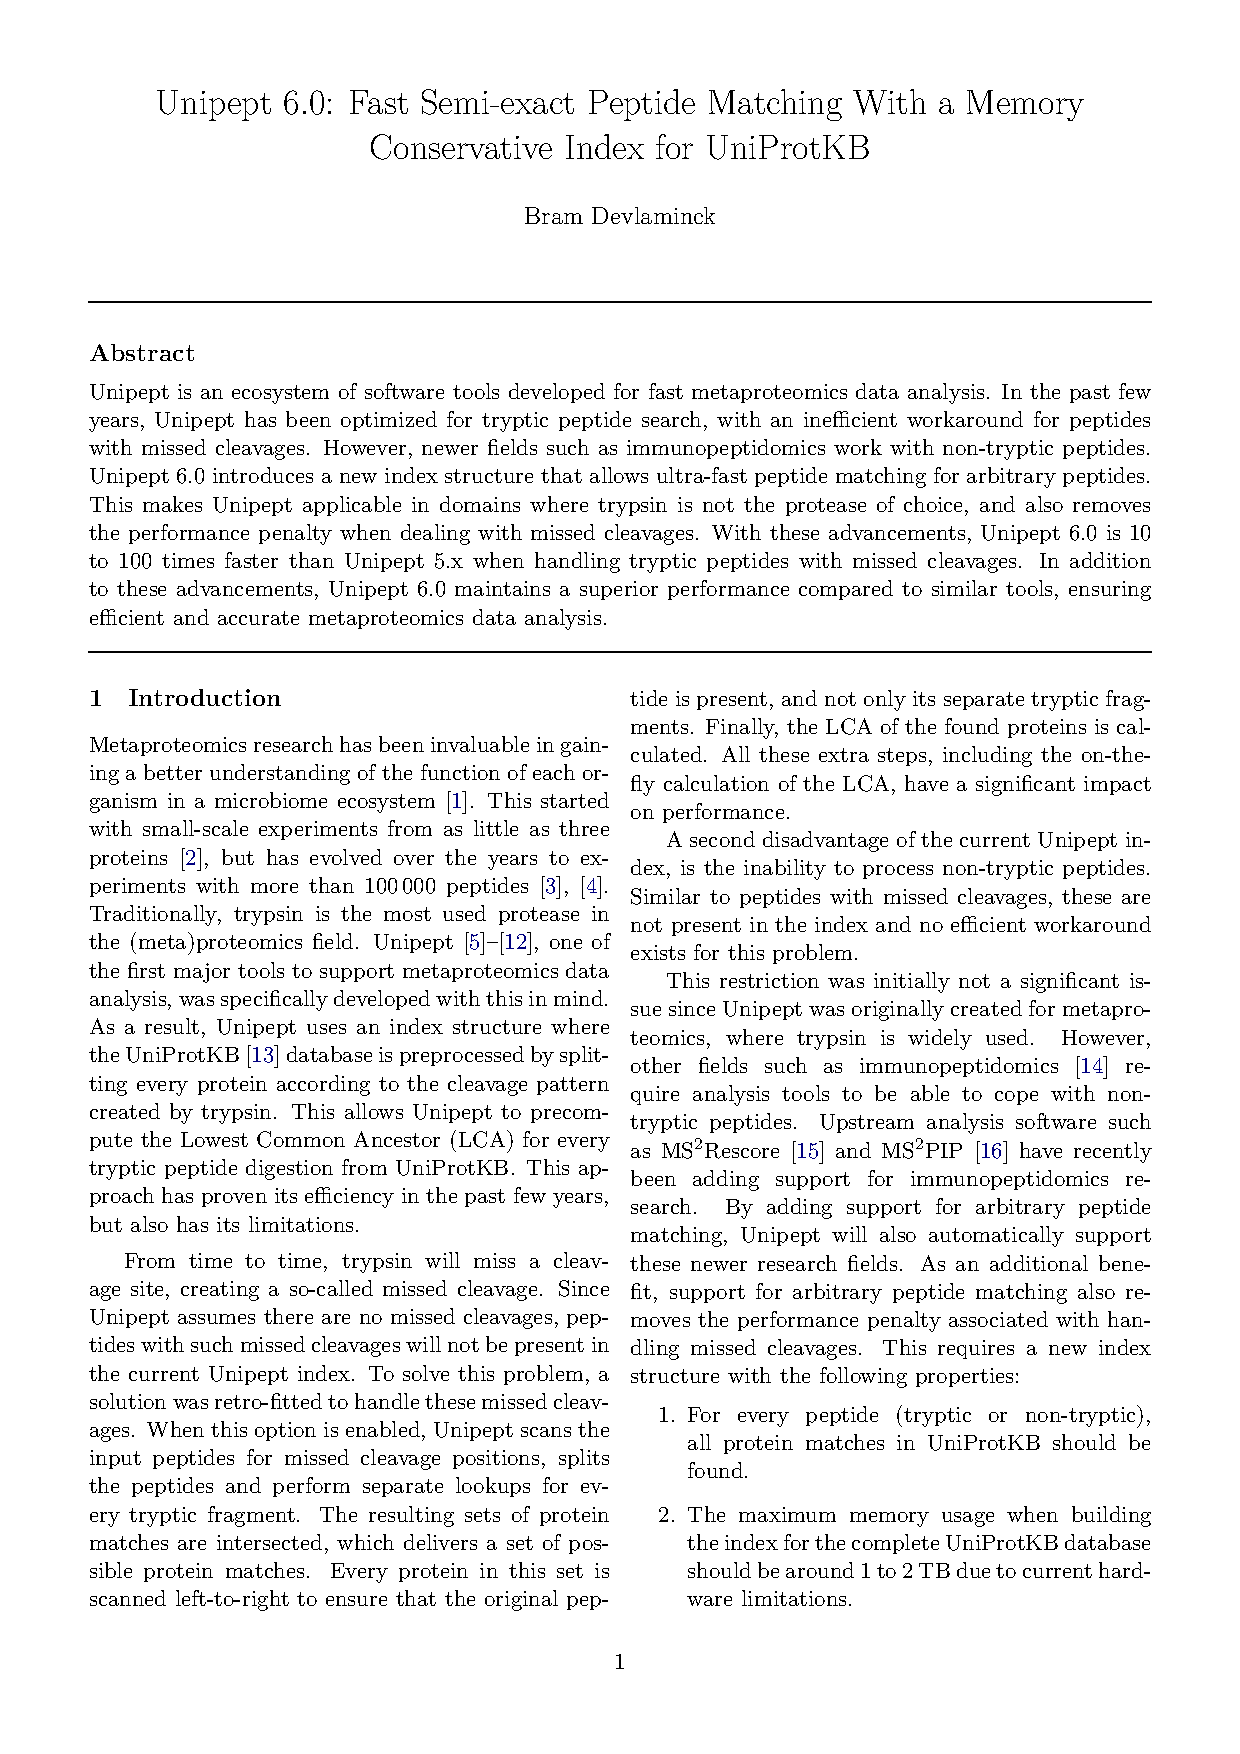
\includepdf[pages=-]{../out/abstract.pdf}


% ------------- CONSENT OF USE -----------
%    \onehalfspacing
    \chapter*{Dankwoord}\label{ch:dankwoord}
Deze masterproef vormt het sluitstuk van de voorbije vijf jaar aan UGent.
Jaren met extreem veel werk, maar ook met fantastische ervaringen.
Deze masterproef is de ultieme combinatie hiervan.
Zonder het begeleidend team van Unipept, waarmee ik wekelijks onze vaste \textit{thesismeeting} had, zou ik nooit zo'n volmaakt resultaat kunnen afleveren.
Daarom wil ik met nadruk mijn promotor prof.~dr.~Peter Dawyndt, copromotor prof.~dr.~ir.~Bart Mesuere en begeleiders dr.~Pieter Verschaffelt en Tibo Vande Moortele bedanken.
Naast alle serieuze en leervolle gesprekken over informatica en metaproteomica, was er altijd plaats voor enkele (of laat ons eerlijk zijn, veel) ongerelateerde side-stories.
\\ \\
Naast deze technische ondersteuning wil ik ook graag mijn ouders en broer bedanken die me de afgelopen vijf jaar bijgestaan hebben in alle stressvolle deadline- en examenperioden.
Hun steun heeft deze perioden aanzienlijk draaglijker gemaakt.
Graag wil ik nog eens afzonderlijk mijn vriendin Claudia bedanken.
Dankzij haar bevat deze masterproef niet enkel minder typfouten en rare zinsconstructies, maar weet ik meer dan ooit dat ik er nooit alleen voor sta, ook in individuele opdrachten zoals deze.
\\ \\
Tot slot wil alle mensen uit de \textit{thesiskelder} bedanken waarmee ik ontelbare uren in de donkerste krochten van S9 gespendeerd heb.
In willekeurige volgorde: Maarten, Stijn, Thomas, Clement en Jonas.
Samen hebben we niet enkel gevloekt op software bugs en vage \LaTeX\ errors, maar ook onvergetelijke herinneringen gemaakt.
Ik ben jullie eeuwig dankbaar voor het gezelschap en jullie input bij een zoveelste dilemma tijdens het maken van deze masterproef.

    \chapter*{Toelating tot bruikleen}

De auteur geeft de toelating deze masterproef voor consultatie beschikbaar te stellen en delen van de masterproef te kopiëren voor persoonlijk gebruik.
Elk ander gebruik valt onder de bepalingen van het auteursrecht, in het bijzonder met betrekking tot de verplichting de bron uitdrukkelijk te vermelden bij het aanhalen van resultaten uit deze masterproef.
\\ \\
Bram Devlaminck \\ \today

    \newpage

% ------------ TABLE OF CONTENTS ---------
    \tableofcontents
    \newpage
    \pagenumbering{arabic}


% =====================================================================
% Main matter
% =====================================================================


    \chapter{Inleiding}\label{ch:introductie}

Eiwitten of proteïnen zijn alomtegenwoordig en spelen een belangrijke rol in ons dagelijkse leven.
Ze garanderen een correcte werking van belangrijke processen binnen elk organisme.
Hieronder vallen de levensprocessen van ons eigen lichaam, maar ook die van dieren, planten, bacteriën en zelfs virussen.
Om deze processen te analyseren zijn er meerdere benaderingen mogelijk.


\section{Genomica, transcriptomica \& proteomica}\label{sec:genomica-transcriptomica-&-proteomica}
Een eerste mogelijkheid is aan de hand van het onderzoeksgebied van de \textbf{proteomica}.
Dit is de studie van alle eiwitten die binnen een enkel organisme tot expressie kunnen komen.
Hierbij probeert men te begrijpen hoe eiwitten in elkaar zitten, hoe deze met elkaar en binnen een bepaalde omgeving met elkaar interageren en wat hun belangrijkste functie is.
In de biologie bestaat er een concept dat de omzetting naar deze eiwitten beschrijft, dit noemt men het centraal dogma.
Wanneer we er een analogie bij betrekken kunnen we centraal dogma omschrijven als het proces dat een gerecht doorloopt in de keuken van een restaurant.
Hierbij zijn de eiwitten het afgewerkte gerecht.
Naast proteomica bestaan er nog twee andere gerelateerde disciplines.
\\ \\
De eerste alternatieve discipline is \textbf{genomica}, het onderzoek naar het genoom.
Het genoom van een organisme is de collectie van al het DNA binnen een organisme.
Dit stelt voor welke proteïnen mogelijks door het organisme geconstrueerd kunnen worden.
Dit is het begin van het proces van het centraal dogma, wanneer we de analogie van eerder erbij betrekken is dit het receptenboek dat alle recepten bevat.
Een belangrijk verschil met proteomica is dat DNA instructies voorstelt voor de productie van alle mogelijke proteïnen die het organisme kan maken.
Het geeft dus geen informatie over de proteïnen die op dat moment in de tijd actief zijn.
Het is een voorstelling van wat het organisme kan, niet wat het op \textit{dit} moment aan het doen is.
Belangrijk is dat ongeveer 98\% van het menselijke genoom niet-coderend is, wat wil zeggen dat dit deel van het DNA niet omgezet kan worden naar een betekenisvolle proteïne.
In de plaats kunnen deze niet-coderende delen omgezet worden naar \textit{regulatory sequences}, niet-coderende genen, of andere componenten.
\\ \\
De andere discipline is de \textbf{transcriptomica}.
Deze discipline onderzoekt het transcriptoom van een organisme, wat de verzameling is van alle RNA moleculen die in het organisme aanwezig zijn.
Het transcriptoom is een belangrijke indicatie van welke delen uit het DNA effectief proteïnen encoderen.
Dit omdat RNA, meer specifiek messenger RNA (mRNA) en transfer RNA (tRNA), een belangrijk onderdeel is van het proces om DNA om te zetten naar proteïnen.
In de restaurant analogie is dit een kopie van één recept uit het receptenboek.
Dit recept beschrijft hoe het gerecht exact gemaakt moet worden.
Een visualisatie van de analogie, en de link met het centraal dogma van de biologie, kan terug gevonden worden in Figuur~\ref{fig:recipe}.
\\ \\
Onze focus ligt vooral binnen het veld van de \textbf{metaproteomica}.
Het \textit{meta} prefix zegt dat de te analyseren stalen niet van één organisme afkomstig zijn, maar van \textbf{meerdere organismen} (typisch binnen hetzelfde ecosysteem).
Dit maakt de analyse moeilijker aangezien proteïnen van verschillende organismen gelijkaardige aminozuursequenties kunnen hebben (al dan niet door toeval).
Meer specifiek is het doel van metaproteomica om op zoek te gaan naar de taxa en functies die horen bij een verzameling van eiwitfragmenten.
Deze eiwitfragmenten noemen we peptides wanneer ze bestaan uit twee of meer aminozuren en hun lengte beperkt blijft.
In de praktijk gaat dit over sequenties van ongeveer 2 tot 50 aminozuren lang.
Een veelvoorkomende categorie van peptiden die we zullen analyseren zijn tryptische peptiden.

\begin{figure}[H]
    \centering
    \includesvg[width=0.8\textwidth]{recipe_book_analogy}
    \caption{Het centraal dogma van de biologie kan makkelijk uitgelegd worden aan de hand van de analogie van een receptenboek. Het DNA komt overeen met het receptenboek dat de recepten bevat voor elk gerecht dat gemaakt kan worden. Eén kopie van één recept komt overeen met RNA. Een afgewerkt gerecht komt dan weer overeen met een proteïne.}
    \label{fig:recipe}
\end{figure}


\section{Tryptische peptiden}\label{sec:tryptische-peptiden}
Tryptische peptiden zijn peptiden die ontstaan na het knippen van proteïnen aan de hand van \textbf{trypsine}.
Dit is een protease (eiwitafbrekend enzym) dat proteïnen opsplitst in meerdere peptiden.
Er bestaan nog andere proteases, maar trypsine is veruit de populairste door zijn eenduidig gedrag en efficiëntie.
\\ \\
Trypsine zal eiwitten knippen na elk voorkomen van lysine (K) of arginine (R) indien het eerstvolgende aminozuur geen proline (P) is.
Deze vuistregel is echter niet perfect.
Soms mist trypsine een locatie waar volgens deze regel geknipt moet worden.
Dit noemen we een \textit{missed cleavage}.
Figuur~\ref{fig:trypsine} bevat een voorbeeld van de werking.

\begin{figure}[H]
    \centering
    \includesvg[width=0.9\textwidth]{trypsine_verwerking}
    \caption{Voorbeeld van de werking van trypsine op 2 proteïnen~\cite{phdPieterUnipept}. De aminozuren in het rood zijn lysine (K) of arginine (R), waarna trypsine knipt (behalve als het eerstvolgende aminzoruur proline (P) is). De tweede proteïne bevat een voorbeeld waar niet geknipt wordt na lysine, doordat het volgende aminozuur proline is.}
    \label{fig:trypsine}
\end{figure}

Om de peptiden uit een experiment te kunnen gebruiken bij computeranalyses moeten deze omgezet worden naar een stringrepresentatie.
Dit is is echter een moeilijk en ingewikkeld proces.
Eerst wordt de massa/ladingsverhouding (m/z) van peptiden aan de hand van een massaspectrometer gemeten.
Daarna worden deze resultaten aan de hand van diverse zoekprocessen (via zogenaamde zoekmachines) omgezet naar de stringvoorstelling van de peptide.
Deze sequenties vormen de input voor tools zoals Unipept.
\\ \\
Eén belangrijke consequentie van het gebruik van een massaspectrometer is dat Isoleucine (I) en Leucine (L) niet uit elkaar gehouden kunnen worden.
Deze aminozuren bestaan uit dezelfde atomen (C\textsubscript{6}H\textsubscript{13}NO\textsubscript{2}), maar deze zijn op een andere manier verbonden.
Hierdoor hebben ze een identieke massa, wat ervoor zorgt dat ze niet te onderscheiden zijn.


\section{Unipept}\label{sec:unipept-introductie}
Unipept~\cite{unipept_orig} biedt een ecosysteem van tools aan om stalen uit het onderzoeksveld van de metaproteomica te analyseren, maar er is ook een onderdeel (UMGAP~\cite{UMGAP_paper}) gericht op het analyseren van stalen uit de metagenomica.

\begin{itemize}
    \item \textbf{Unipept Web application~\cite{unipept_orig, unipept_web, unipept_tutorial, unipept_4}} Dit is de originele Unipept tool en is publiek beschikbaar op \url{https://unipept.ugent.be}.
    Met de gebruiksvriendelijke \textit{user interface} wordt analyseren van metaproteomica data beschikbaar gesteld.
    De resultaten van deze analyse worden aan de hand van visualisaties en tabellen aan de gebruiker voorgesteld.
    Deze kunnen vervolgens makkelijk geëxporteerd worden (bijv.~voor analyse in andere tools).
    \item \textbf{Unipept CLI\footnote{\textit{commandline interface}}~\cite{unipept_cli}} Dit is een \textit{power-user} tool voor de commandolijn om analyses uit te voeren op grotere stalen.
    \item \textbf{Unipept API\footnote{\textit{application programming interface}}~\cite{unipept_api, unipept_cli}} Dit is een collectie van \textit{endpoints} die andere applicaties (inclusief de Unipept CLI), toelaat om de functionaliteit van Unipept te integreren.
    \item \textbf{Unipept Desktop~\cite{unipept_desktop, unipept_desktop_2}} Dit is de recentste toevoeging aan het Unipept ecosysteem en laat toe dat onderzoekers niet noodzakelijk met de Unipept servers moeten communiceren om analyses uit te voeren.
    Deze applicatie combineert de voordelen van de web app, CLI en API en laat toe om lokaal stalen te analyseren, gebruikmakende van een gebruiksvriendelijke UI\@.

\end{itemize}

Op dit moment is Unipept \textbf{exclusief gericht op de analyse van tryptische peptiden}.
De reden hiervoor is de manier waarop de achterliggende indexstructuur opgebouwd wordt.
Dit opbouwen gaat in grote lijnen als volgt:

\begin{enumerate}
    \item Haal alle proteïnen en bijbehorende taxonomische en functionele annotaties op uit de UniProtKB databank~\cite{UniprotKB}.
    \item Splits deze proteïnen volgens de vuistregel die trypsine nabootst.
    \item Sla alle resulterende tryptische peptiden op in een databank, samen met hun voorberekende taxonomische en functionele metadata.
\end{enumerate}

Deze aanpak heeft als voordeel dat we op een efficiënte manier tryptische peptiden kunnen opzoeken (samen met de bijbehorende annotaties).
Er is echter een belangrijke keerzijde aan deze manier van werken.
Het zoeken van niet-tryptische peptiden (hieronder vallen ook peptiden met \textit{missed cleavage}) is problematisch.
Dit komt doordat tijdens het opbouwen van de Unipept indexstructuur de vuistregel strikt gevolgd wordt, en elke peptide in de indexstructuur strikt tryptisch is.
Op basis hiervan worden de taxonomische en functionele annotaties voor elke tryptische peptide voorberekend.
\\ \\
Op dit moment is er wel een \textit{workaround} die toelaat om peptiden met \textit{missed cleavages} toch te zoeken.
Dit heeft echter wel een significante impact op de performantie.
Deze verminderde performantie bij \textit{missed cleavages}, in combinatie met het compleet ontbreken van een manier om willekeurig gesplitste peptiden te zoeken, verklaart de nood aan een nieuwe indexstructuur.
\\ \\
Voor een gedetailleerdere beschrijving van Unipept en het onderzoeksveld van metaproteomica is het aangeraden om de inleiding van het doctoraat van Dr.~Pieter Verschaffelt te lezen~\cite{phdPieterUnipept}.
Dit vormde een duidelijke en goede basis voor deze inleiding.


\section{Probleemstelling}\label{sec:probleemstelling}
In deze masterproef zoeken we een oplossing voor het snel terugvinden van \textbf{willekeurige peptiden} in een eiwitdatabank.
Bij het vinden van een match moet het daarna mogelijk zijn de informatie op te halen die hoort bij alle proteïnen waarin de peptide voorkomt.
Binnen het onderzoeksgebied van de informatica kunnen we dit probleem als volgt herformuleren:
``In een grote verzameling van middellange strings (alle eiwitten in onze databank), moeten we voor een verzameling van korte strings (peptiden) terugvinden in welke van deze middellange strings ze voorkomen.''
We willen echter niet alleen maar vinden van welke proteïnen een peptide deel is.
Ook de bijbehorende taxonomische en functionele annotaties van de gematchte proteïne moeten zo snel mogelijk te vinden zijn.
Deze gevonden annotaties moeten efficiënt verwerkt kunnen worden om zo efficiënt het eindresultaat te bekomen.
Om dit te realiseren, worden waar mogelijk annotaties geaggregeerd tijdens het opbouwen van de indexstructuur.
\\ \\
Belangrijk hierbij is dat dit alles niet alleen \textbf{snel} gebeurt, maar dat we ook proberen \textbf{het vereiste geheugen tot een minimum te beperken}.
Wat als acceptabel beschouwd wordt, hangt af van de omgeving waarin de analyses uitgevoerd worden.
Voor stalen die geanalyseerd worden op een PC m.b.v.~Unipept Desktop is dit $\pm$ 16 GB RAM\@.
Voor grotere stalen waarvan de analyse op de Unipept servers uitgevoerd wordt mikken we op 0.5-2 TB geheugengebruik.
Dit komt overeen met een realistische configuratie voor een server die gericht is op het uitvoeren geheugenintensieve taken.
\\ \\
Tot slot willen we ook \textbf{semi-exacte matching} toevoegen tijdens het zoeken.
Hierbij willen we de mogelijkheid aanbieden om Isoleucine (I) en Leucine (L) gelijk te stellen aan elkaar.
Wanneer deze gelijkgesteld zijn wil dit zeggen dat op elke plaats waar een I staat, ook een L toegelaten wordt, en omgekeerd.
Door dit te doen kunnen we de beperkingen van een massaspectrometer opvangen.
\\ \\
Om dit allemaal te bereiken is het doel van deze thesis om meerdere datastructuren uit te werken, te implementeren in Rust, en tot slot te testen.
Het gebruik van Rust laat ons toe om extreem hoge performantie te verkrijgen (vergelijkbaar met C en C++~\cite{rustPerformantie}) in combinatie met \textit{memory safety}\footnote{\textit{Memory safety} is een eigenschap die verzekert dat programma's enkel gebruik kunnen maken van geldige geheugenlocaties en geen \textit{undefined behaviour} zoals \textit{buffer overflows}, \textit{dangling pointers} en andere geheugen gerelateerde fouten kunnen vertonen.}.
Bovendien zijn sommige delen van Unipept al geschreven in Rust (zie UMGAP~\cite{UMGAP_paper, UMGAP_source}).
Dit laat toe om waar mogelijk bestaande code te hergebruiken.


\section{Benchmarkdatasets}\label{sec:datasets}
Om de snelheid, het geheugengebruik en de correctheid van de onderzochte indexstructuren en zoekalgoritmen te bepalen zullen we \textbf{twee soorten benchmarkbestanden} gebruiken.
De eerste soort zijn de \textbf{proteïnedatabanken} waarmee we de indexstuctuur opbouwen.
De grootte van deze indexstructuur is het primaire criterium aangezien deze \textbf{volledig in het werkgeheugen} moet passen, wat een harde limiet is.
Indien de index niet in het geheugen past, zal het programma niet uitgevoerd kunnen worden (of met een erg grote performance-penalty wanneer swapruimte\footnote{Dit is wanneer een computer schijfruimte gebruikt om het tekort aan RAM-geheugen op te vangen.} gebruikt wordt).
De andere soort bestanden bevatten de peptiden die we gaan proberen terugvinden in de indexstructuur.
Daarom zullen we voor de rest van deze masterproef hiernaar verwijzen als \textbf{peptidebestanden}.
Het hoofddoel van deze peptidebestanden is om de zoekperformantie te testen.
De tijd nodig om te zoeken is een zachte limiet aangezien we mikken voor hoge performantie, maar tragere code heeft enkel als gevolg dat een gebruiker langer moet wachten.
Alle bestanden die in de volgende secties besproken worden, kunnen teruggevonden worden in onze GitHub repository\footnote{\url{https://github.com/BramDevlaminck/Thesis_benchmarkdata}}.

\subsection{Proteïnedatabanken}\label{subsec:proteine-databanken}
Om te testen hoe goed een implementatie is en hoe deze zich verhoudt ten opzichte van bestaande implementaties, is het belangrijk om representatieve datasets te gebruiken.
Deze datasets zijn allemaal eiwitdatabanken die een subset vormen van \textbf{UniProtKB} (meer specifiek UniProtKB 2023\_04)~\cite{UniprotKB}.
UniProtKB zelf bestaat uit twee onderdelen (gegeven statistieken zijn voor release 2023\_04).
\begin{enumerate}
    \item \textbf{Swiss-Prot}: Dit is een kleinere, manueel gecureerde dataset met 570\thinspace157 eiwitsequenties.
    \item \textbf{TrEMBL}: Deze dataset bevat 251\thinspace600\thinspace768 sequenties en is dus veel groter dan Swiss-Prot.
    Een bijkomend verschil is dat deze dataset \textbf{niet} manueel gecureerd is, maar algoritmisch geannoteerd werd.
\end{enumerate}
Uiteindelijk is het doel om een indexstructuur voor UniProtKB op te bouwen waarbij de probleemstelling opgelost is.
UniProtKB is echter veel te groot om mee te werken tijdens het testen.
In plaats hiervan gebruiken we tijdens het ontwikkelen twee kleinere subsets van UniProtKB\@.
Eerst wordt een overzicht gegeven van de belangrijkste eigenschappen van UniProtKB, om daarna dieper in te gaan op de twee gebruikte subsets tijdens het testen.

\paragraph{UniProtKB}
Tabel~\ref{tab:uniprotKB_eigenschappen} bevat een overzicht van de belangrijkste statistieken voor de volledige UniProtKB 2023\_04 databank.
Belangrijk om op te merken is dat de totale databank uit 86\thinspace805\thinspace673\thinspace041 aminozuren bestaat.
Omgerekend is dit 86.81 GB aangezien een karakter opgeslagen wordt in één byte.
Dit verklaart onmiddellijk de keuze om gebruik te maken van kleinere datasets tijdens het testen.

\begin{table}[h!]
    \centering
    \begin{tabular}{ l l }
        Metriek                   & Waarde                                       \\
        \hline\hline
        Totaal aantal sequenties  & 248\thinspace842\thinspace516                \\
        Totale lengte             & 86\thinspace805\thinspace673\thinspace041 aa \\
        Minimale proteïnelengte   & 1 aa                                         \\
        Maximale proteïnelengte   & 45\thinspace354 aa                           \\
        Gemiddelde proteïnelengte & 348.84 aa                                    \\
        Mediaan proteïnelengte    & 278 aa                                       \\
        \hline
    \end{tabular}
    \caption{Eigenschappen van de volledige UniProtKB 2023\_04 databank. De afkorting \textit{aa} staat voor \textit{amino acids}.}
    \label{tab:uniprotKB_eigenschappen}
\end{table}

In Figuur~\ref{fig:uniprot_aminozuur} en~\ref{fig:uniprot_length} is een gedetailleerder overzicht van de aminozuurdistributie en verdeling van de proteïnelengtes terug te vinden.

\begin{figure}[h]
    \centering
    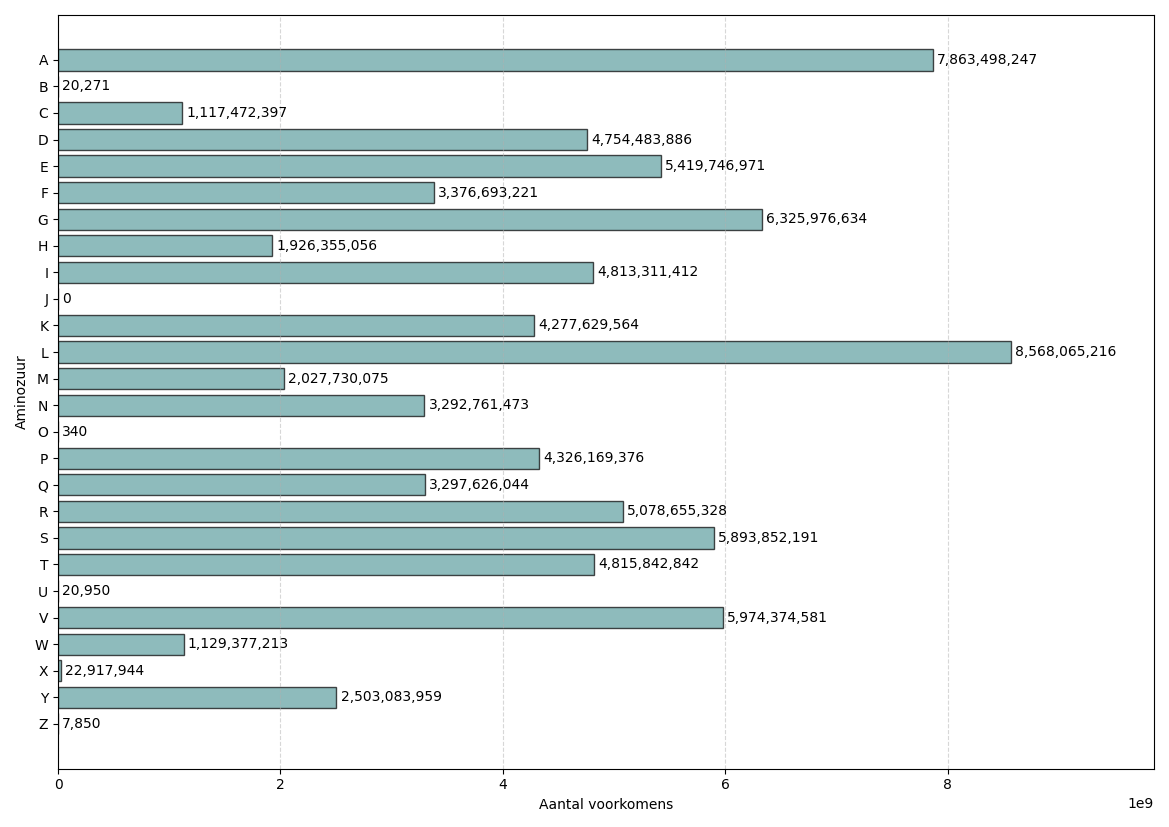
\includegraphics[width=0.6\linewidth]{uniprotKB_aminozuur_voorkomens}
    \caption{Aantal voorkomens per aminozuur voor alle proteïnen in de UniProtKB (2023\_04) databank.}
    \label{fig:uniprot_aminozuur}
\end{figure}

\begin{figure}[h]
    \centering
    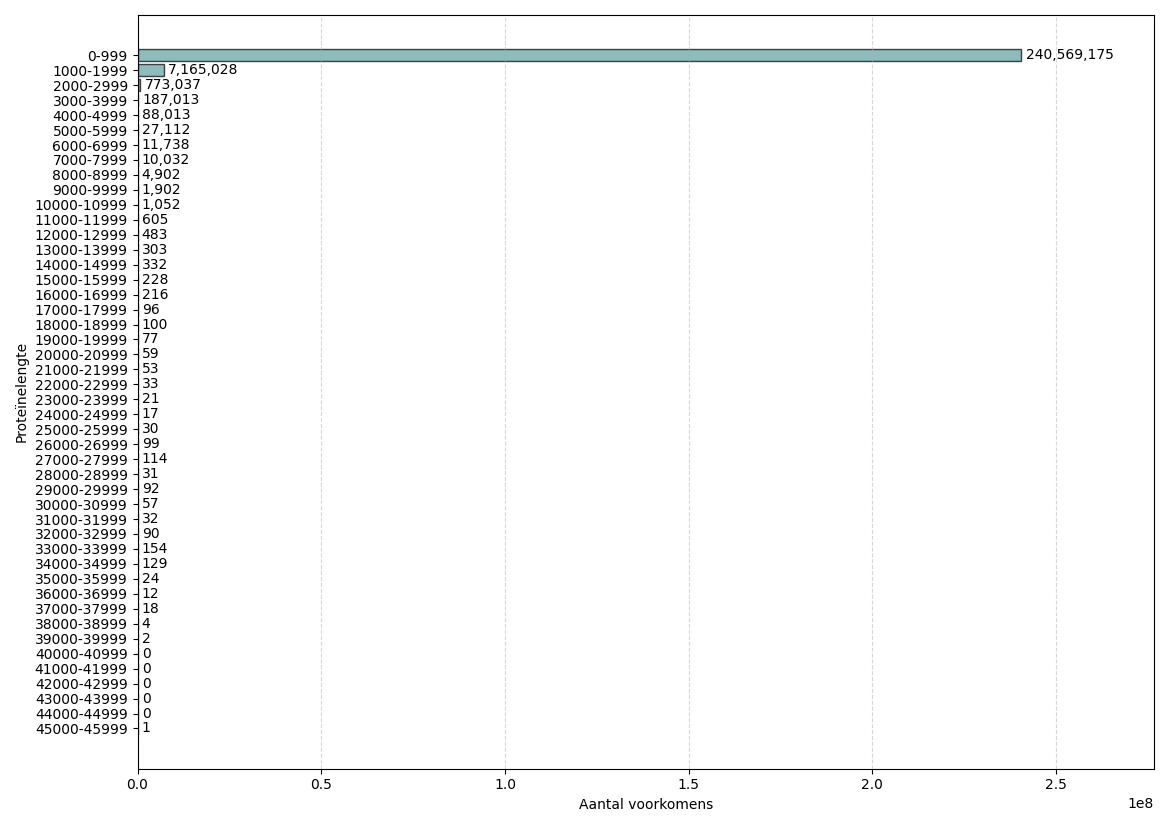
\includegraphics[width=0.95\linewidth]{uniprotKB_length_distribution_large}
    \makebox[0pt][r]{% Similar to \llap
        \raisebox{2.2em}{%
            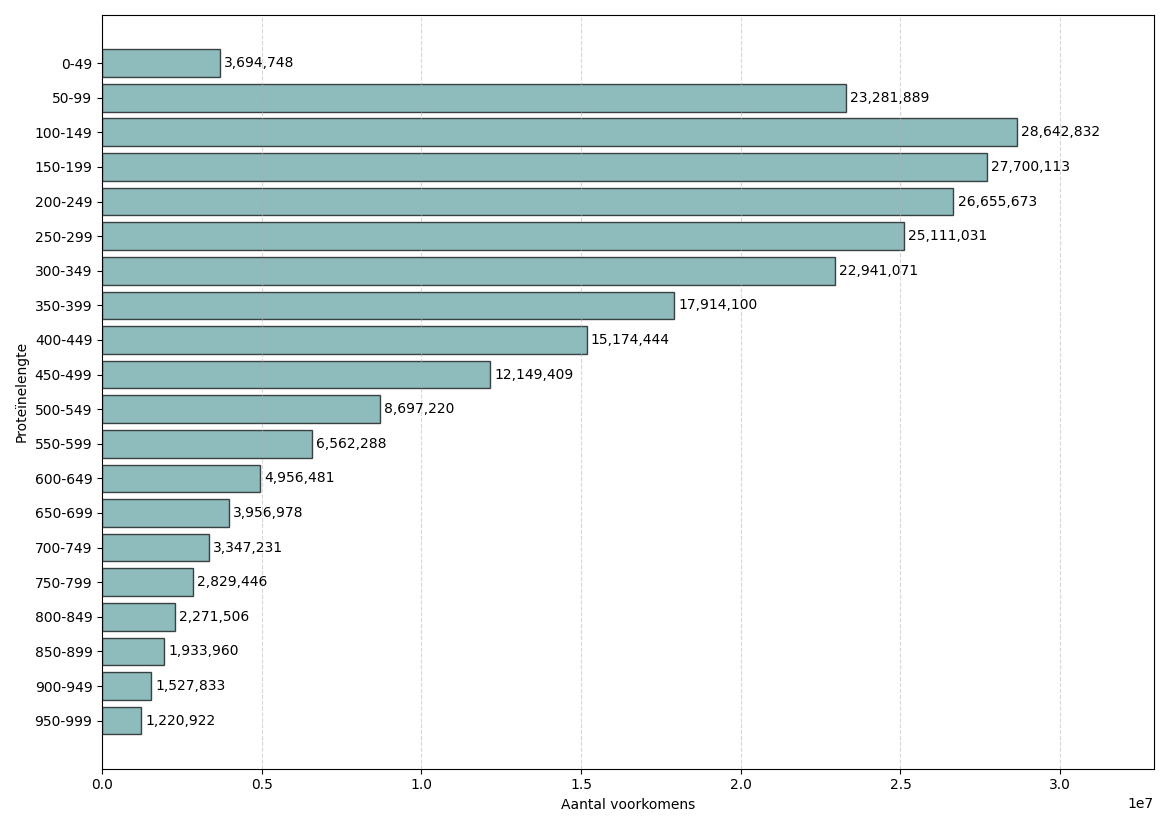
\includegraphics[width=0.65\linewidth]{uniprotKB_length_distribution_small}% Inserted image/inset
        }\hspace*{2em}%
    }%
    \caption{Lengtedistributie van de proteïnen in de UniProtKB (2023\_04) databank. De kleinere grafiek bevat een gedetailleerder overzicht van de distributie in het interval $[0, 1000[$.}\label{fig:uniprot_length}
\end{figure}

\paragraph{Swiss-Prot} Deze databank is één van de twee standaardonderdelen van UniProtKB\@.
Een kort overzicht van alle statistieken is terug te vinden in Tabel~\ref{tab:swissprot_eigenschappen}.
Figuur~\ref{fig:swissprot_aminozuur} en Figuur~\ref{fig:swissprot_length} geven meer inzicht in de distributie van de aminozuren en lengte van de proteïnen.

\begin{table}[h]
    \centering
    \begin{tabular}{l l}
        Metriek                   & Waarde                           \\
        \hline\hline
        Totaal aantal sequenties  & 569\thinspace619                 \\
        Totale lengte             & 205\thinspace954\thinspace074 aa \\
        Minimale proteïnelengte   & 2 aa                             \\
        Maximale proteïnelengte   & 35\thinspace213 aa               \\
        Gemiddelde proteïnelengte & 361.56 aa                        \\
        Mediaan proteïnelengte    & 295 aa                           \\
        \hline
    \end{tabular}
    \caption{Eigenschappen van de Swiss-Prot databank (UniProtKB 2023\_04). De afkorting \textit{aa} staat voor \textit{amino acids}.}
    \label{tab:swissprot_eigenschappen}
\end{table}


\begin{figure}[h]
    \centering
    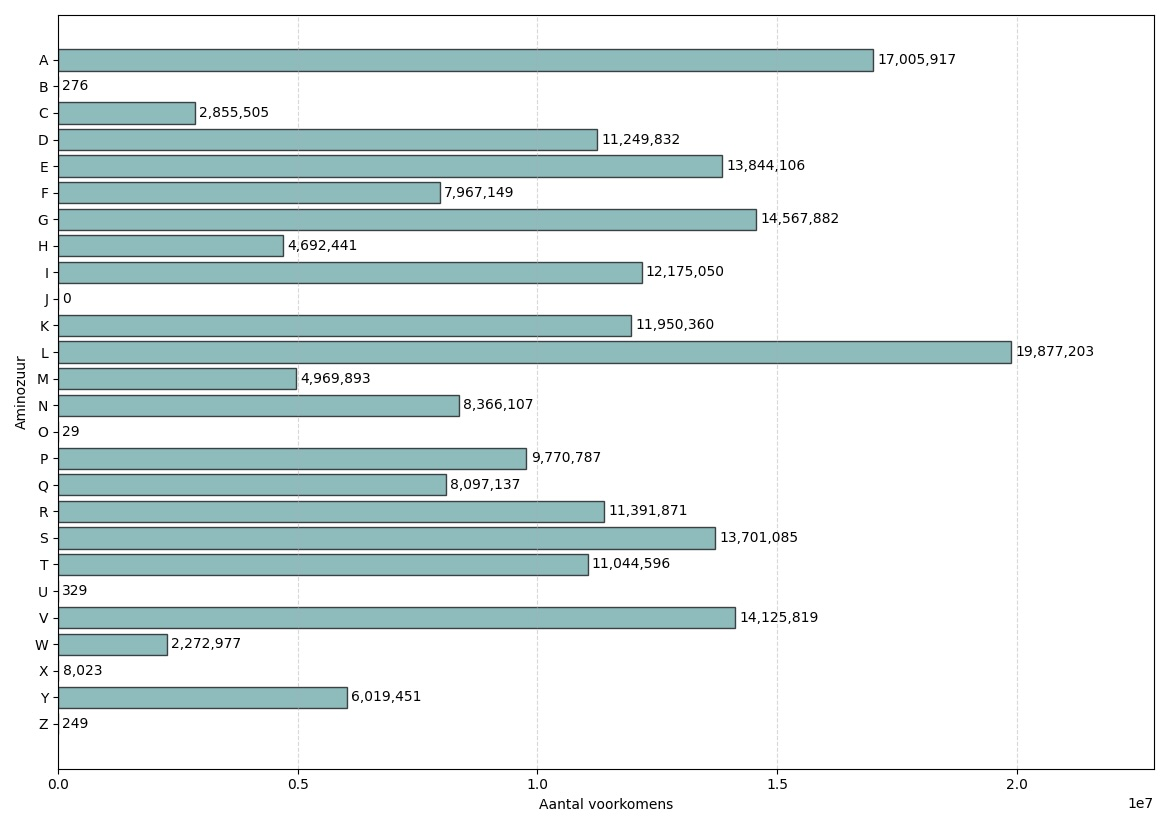
\includegraphics[width=0.6\linewidth]{swissprot_aminozuur_voorkomens}
    \caption{Aantal voorkomens per aminozuur voor alle proteïnen in de Swiss-Prot databank uit UniProtKB 2023\_04.}
    \label{fig:swissprot_aminozuur}
\end{figure}

\begin{figure}[h]
    \centering
    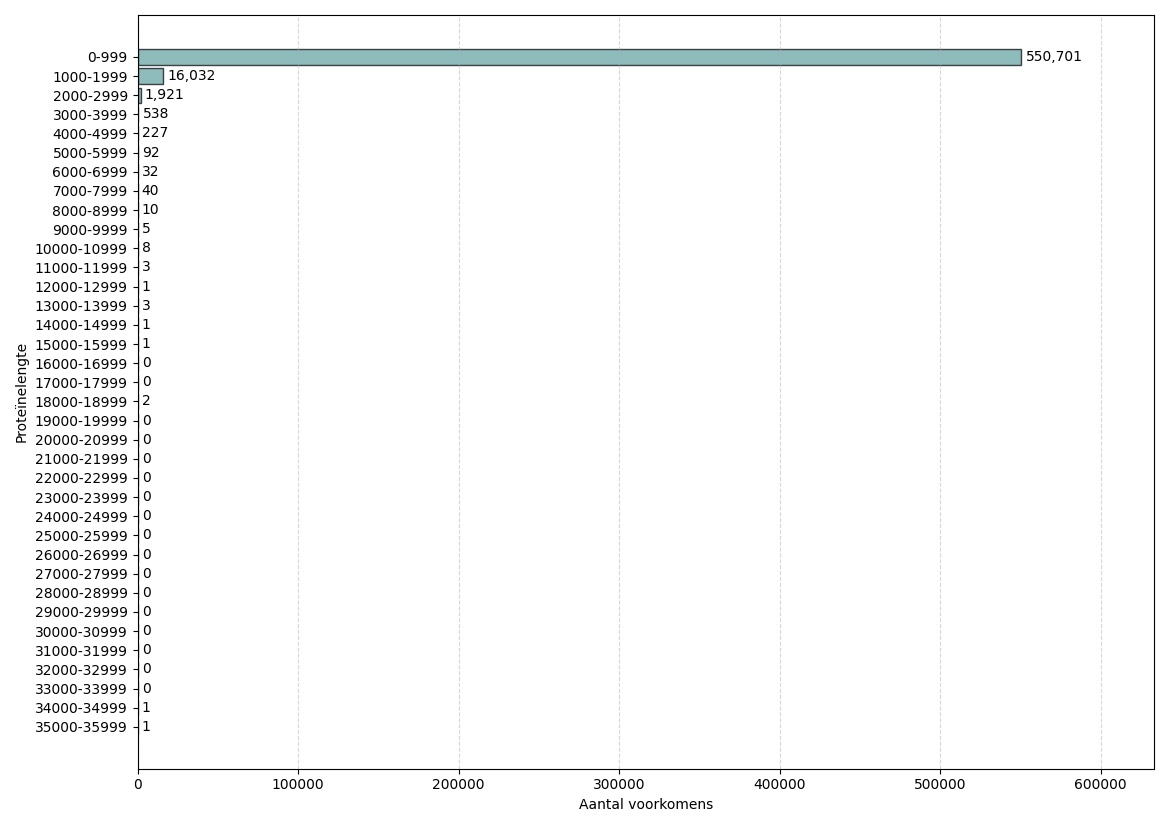
\includegraphics[width=0.95\linewidth]{swissprot_length_distribution_large}
    \makebox[0pt][r]{% Similar to \llap
        \raisebox{2.2em}{%
            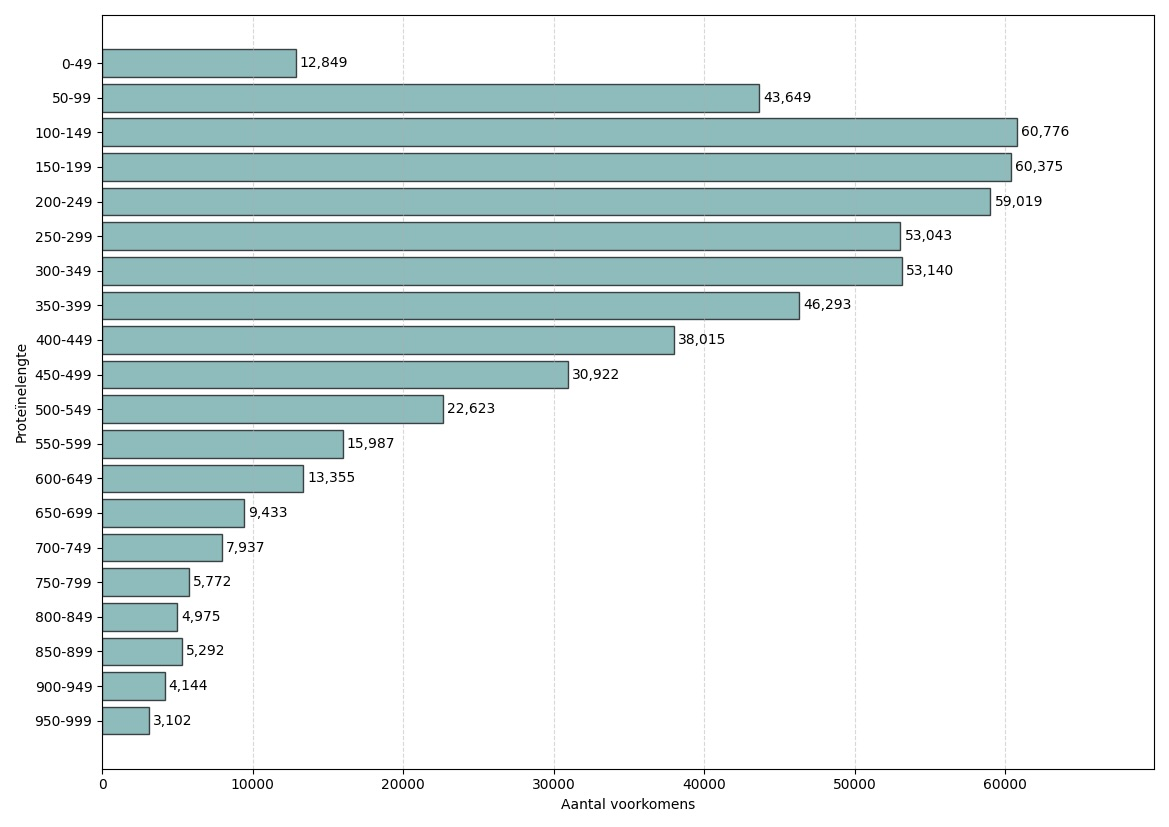
\includegraphics[width=0.65\linewidth]{swissprot_length_distribution_small}% Inserted image/inset
        }\hspace*{2em}%
    }%
    \caption{Lengtedistributie van de proteïnen in de Swiss-Prot databank. De kleinere grafiek bevat een gedetailleerder overzicht van de distributie in het interval $[0, 1000[$.}\label{fig:swissprot_length}
\end{figure}

Doordat het gebruikte invoerbestand reeds verwerkt werd door een deel van de Unipept pipeline, is er een klein verschil tussen het totaal aantal sequenties in Tabel~\ref{tab:swissprot_eigenschappen} en wat eerder aangegeven werd.
Hierbij worden onder andere sequenties met een onbekend taxon id verwijderd (538 in totaal), wat het kleine verschil verklaart.

\paragraph{Human-Prot} Deze dataset is samengesteld aan de hand van drie referentiedatabanken afkomstig uit UniProtKB\@.
Dit zijn de Human Genome~\cite{proteomes_homo_sapiens}, Influenza B~\cite{proteomes_infuenza_b} en Human Papillomavirus~\cite{proteomes_human_papillomavirus} databank.
Opnieuw komen deze allemaal uit UniProtKB 2023\_04.
\\ \\
Deze Human-Prot databank is kleiner dan Swiss-Prot, waardoor het testen tijdens ontwikkeling sneller is.
Tabel~\ref{tab:humanprot_eigenschappen} somt enkele belangrijke metrieken op over deze dataset.
Figuur~\ref{fig:humanprot_aminozuur} en~\ref{fig:humanprot_length} gaan dieper in op een aantal details.
\\
\begin{table}[ht]
    \centering
    \begin{tabular}{ l l }
        Metriek                   & Waarde                          \\
        \hline\hline
        Totaal aantal sequenties  & 82\thinspace695                 \\
        Totale lengte             & 30\thinspace293\thinspace046 aa \\
        Minimale proteïnelengte   & 2 aa                            \\
        Maximale proteïnelengte   & 35\thinspace991 aa              \\
        Gemiddelde proteïnelengte & 366.32 aa                       \\
        Mediaan proteïnelengte    & 204 aa                          \\
        \hline
    \end{tabular}
    \caption{Eigenschappen van de Human-Prot databank (UniProtKB 2023\_04). De afkorting \textit{aa} staat voor \textit{amino acids}.}
    \label{tab:humanprot_eigenschappen}
\end{table}

\begin{figure}[ht]
    \centering
    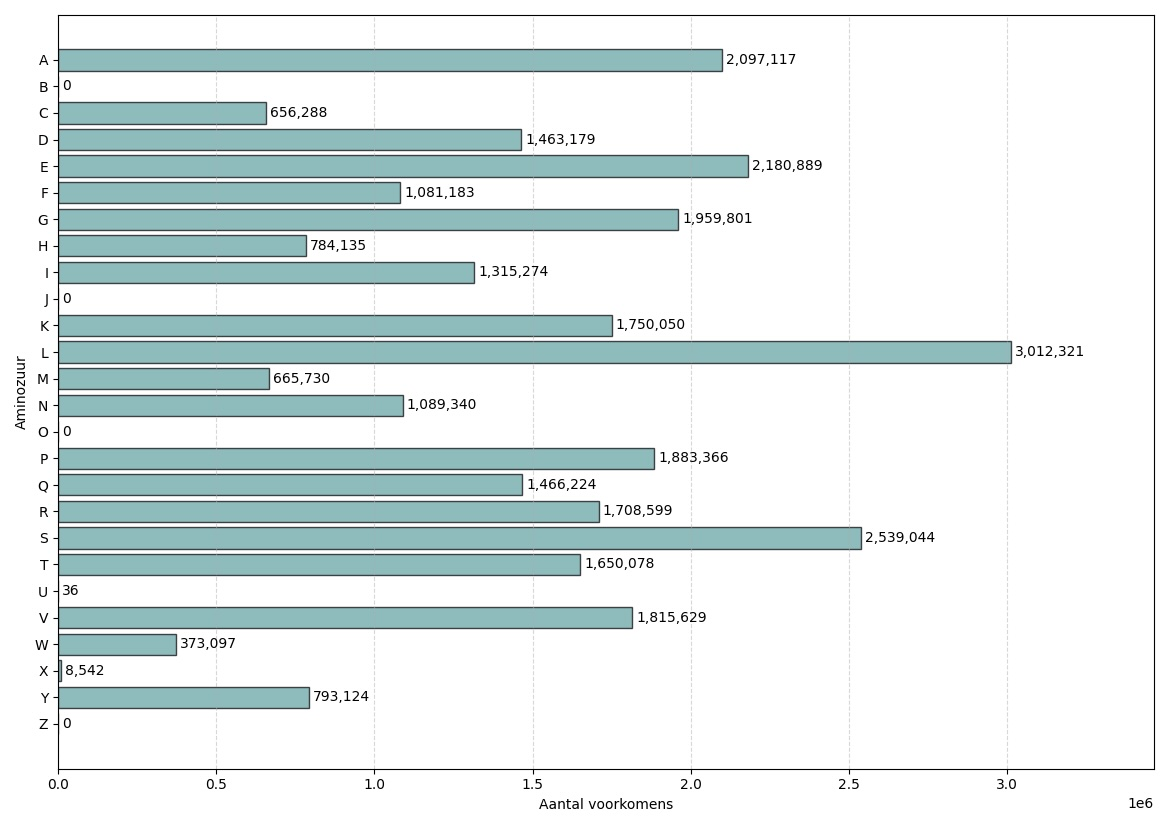
\includegraphics[width=0.7\linewidth]{humanprot_aminozuur_voorkomens}
    \caption{Aantal voorkomens per aminozuur voor alle proteïnen in de Human-Prot databank.}
    \label{fig:humanprot_aminozuur}
\end{figure}

\begin{figure}[ht]
    \centering
    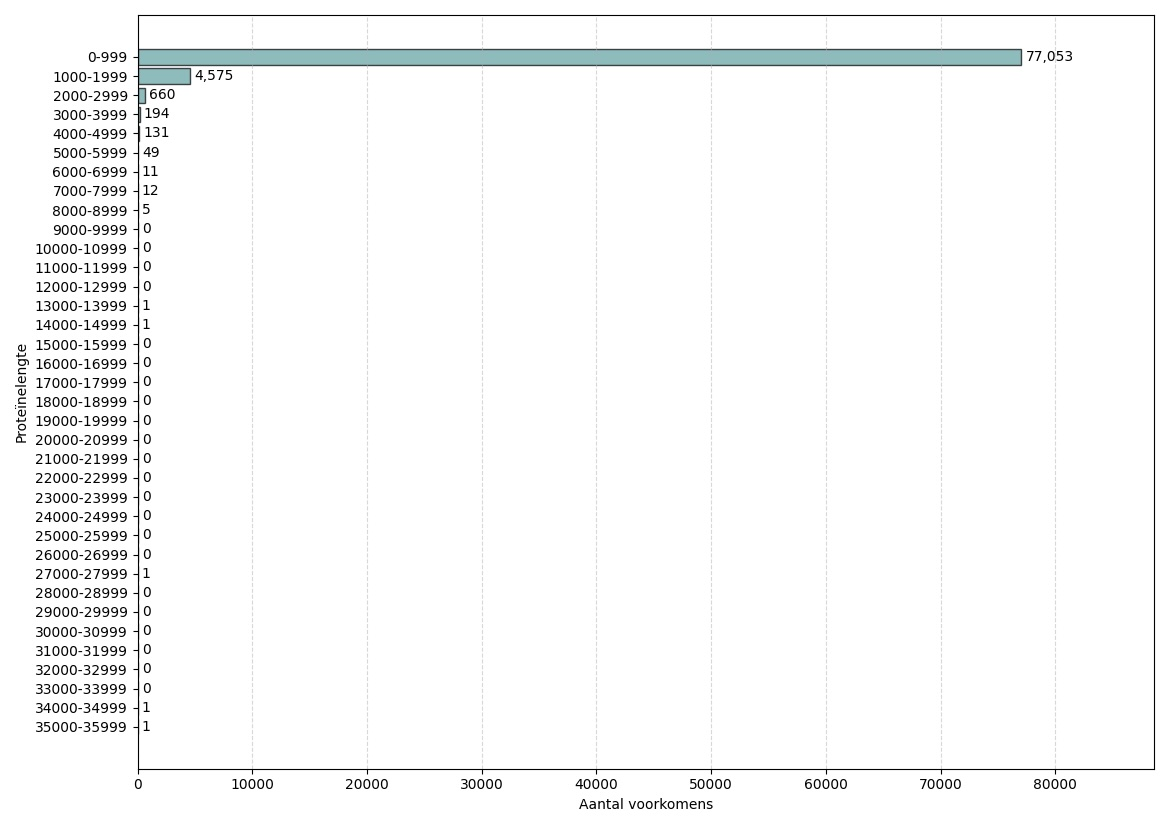
\includegraphics[width=0.95\linewidth]{humanprot_length_distribution_large}
    \makebox[0pt][r]{% Similar to \llap
        \raisebox{2.2em}{%
            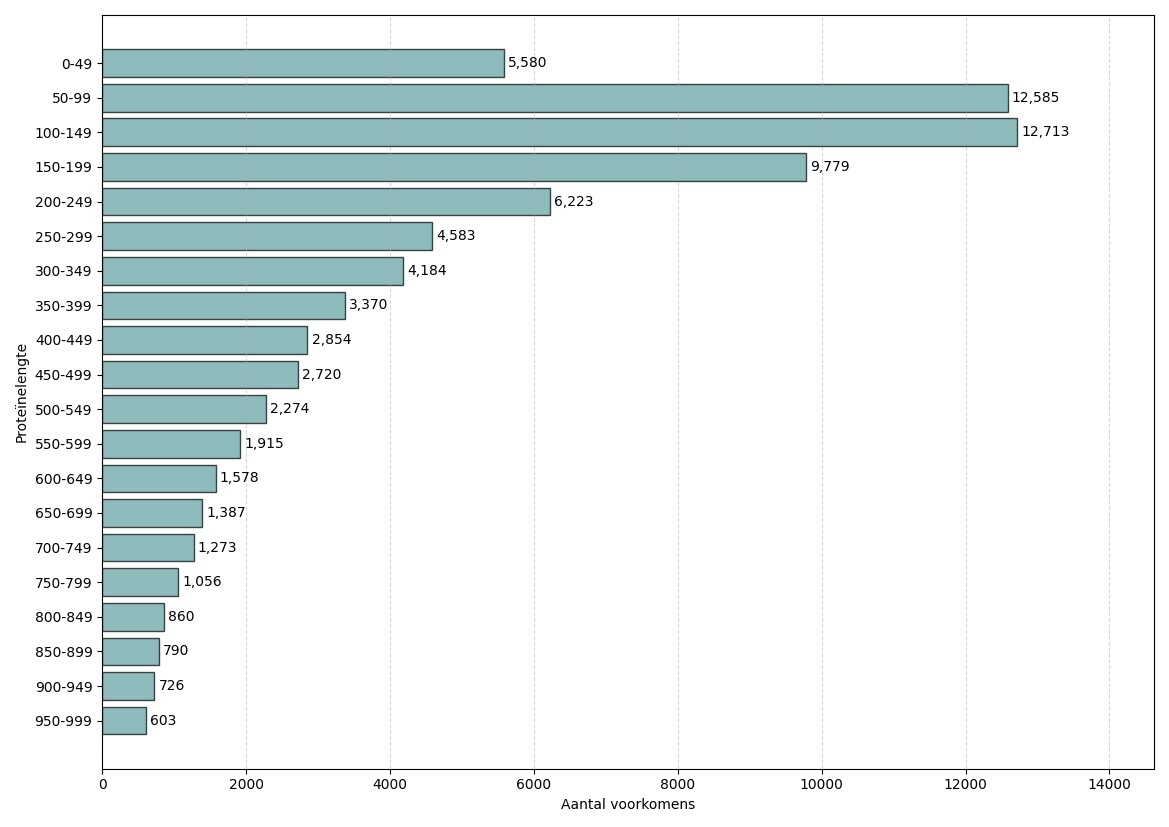
\includegraphics[width=0.65\linewidth]{humanprot_length_distribution_small}% Inserted image/inset
        }\hspace*{2em}%
    }%
    \caption{Lengtedistributie van de proteïnen in de Human-Prot databank. De kleinere grafiek bevat een gedetailleerder overzicht van de distributie in het interval $[0, 1000[$.}\label{fig:humanprot_length}
\end{figure}

We kunnen concluderen dat zo goed als \textbf{alle letters gebruikt} worden (ook al zijn er maar 20 aminozuren).
Dit komt doordat sommige letters eigenlijk een soort wildcard voorstellen.
Zo staat ``X'' voor elk mogelijk aminozuur, ``Z'' voor ``Q'' of ``E'',\ldots~\cite{amino_acid_codes}.
\\ \\
Verder valt ook te zien dat de verdeling van de proteïnelengtes in de UniProtKB, Swiss-Prot en Human-Prot datasets vergelijkbaar zijn.
Met andere woorden: \textbf{Swiss-Prot en Human-Prot zijn een representatieve kleinere voorstelling van UniProtKB\@}.
Dit laat ons toe om gebruik te maken van de Swiss-Prot en Human-Prot eiwitdatabanken en later de resultaten te veralgemenen en op te schalen naar UniProtKB\@.

\subsection{Peptidebestanden}\label{subsec:peptide-zoek-bestanden}
De zoekperformantie van onze indexstructuur is een erg belangrijk aspect.
Om dit te meten, hebben we bij elke eiwitdatabank een lijst aan peptiden die we proberen te zoeken.
Zowel voor de Swiss-Prot als Human-Prot databank zijn enkele datasets opgesteld.

\subsubsection{Swiss-Prot}
Voor deze proteïnedatabank hebben we enkele peptidebestanden voorzien.
Twee bestanden die gesampled zijn en een reeks aan real-life stalen.
De twee artificiële bestanden zijn zo gekozen dat de ene enkel tryptische peptiden bevat, terwijl de andere ook peptiden bevat met \textit{missed cleavages}.
De eerste kan dus op dit moment al efficiënt door Unipept verwerkt worden, terwijl dit voor de tweede niet mogelijk is.

\paragraph{Artificiële stalen}
Tabel~\ref{tab:artifiele_bestanden_statistieken} bevat in kolom twee en drie een kort overzicht met statistieken voor deze gesamplede bestanden.

\begin{table}[H]
    \centering
    \begin{tabular}{l l l l}
        Metriek                    & Swiss-Prot-TRYP                & Swiss-Prot-MC                  & Human-Prot                                  \\
        \hline\hline
        Totaal aantal sequenties   & 100\thinspace000               & 100\thinspace000               & 250\thinspace000                            \\
        Totale lengte              & 1\thinspace605\thinspace909 aa & 2\thinspace544\thinspace356 aa & 2\thinspace458\thinspace834\thinspace046 aa \\
        Minimale peptidelengte     & 5 aa                           & 5 aa                           & 1 aa                                        \\
        Maximale peptidelengte     & 50 aa                          & 93 aa                          & 12 aa                                       \\
        Gemiddelde peptidelengte   & 16.06 aa                       & 25.44 aa                       & 9.84 aa                                     \\
        Mediaan peptidelengte      & 13 aa                          & 23 aa                          & 10 aa                                       \\
        Aantal vindbare peptiden   & 67\thinspace375                & 62\thinspace581                & 250\thinspace000                            \\
        Aantal tryptische peptiden & 100\thinspace000               & 4107                           & 102\thinspace659                            \\
        \hline
    \end{tabular}
    \caption{Eigenschappen van de verschillende peptidebestanden. \textit{Swiss-Prot-TRYP} bevat de statistieken voor het Swiss-Prot peptidebestand met enkel tryptische peptiden. Hierbij komen er dus geen \textit{missed cleavages} voor. \textit{Swiss-Prot-MC} bevat net wel \textit{missed cleavages}. De laatste kolom bevat de statistieken voor het peptidebestand dat hoort bij de Human-Prot eiwitdatabank. De afkorting \textit{aa} staat voor \textit{amino acids}.}
    \label{tab:artifiele_bestanden_statistieken}
\end{table}

\paragraph{Experimentele stalen}
Om de performantie beter te beoordelen, gebruiken we ook enkele stalen uit experimenten met een kleine micro-organisme gemeenschap, namelijk SIHUMIx\footnote{Simplified human intestinal microbiota}~\cite{SIHUMI_first_introduction, SIHUMI_frequently_used}.
Aangezien dit effectieve stalen zijn, bevatten deze \textit{missed cleavages} die natuurlijk ontstaan zijn.
Tabel~\ref{tab:sihumi_zoekbestanden} bevat de belangrijkste statistieken voor elk peptidebestand.
Deze peptidebestanden worden in combinatie met de Swiss-Prot proteïnedatabank gebruikt tijdens het testen.

\begin{table}[H]
    \begin{minipage}{\linewidth}
        \centering
        \resizebox{\textwidth}{!}{ % use resizebox to textwidth since this needs to be scaled down in size a bit because otherwise it does not fit on the width of the screen
            \begin{tabular}{ l l l l l l l }
                Metriek                    & SIHUMI 03           & SIHUMI 05           & SIHUMI 05           & SIHUMI 08           & SIHUMI 11           & SIHUMI 14           \\
                \hline\hline
                Totaal aantal sequenties   & 25\thinspace000     & 25\thinspace000     & 24\thinspace424     & 25\thinspace000     & 24\thinspace998     & 25\thinspace000     \\
                Totale lengte              & 420\thinspace544 aa & 420\thinspace423 aa & 373\thinspace633 aa & 316\thinspace114 aa & 366\thinspace894 aa & 430\thinspace674 aa \\
                Minimale peptidelengte     & 6 aa                & 6 aa                & 6 aa                & 6 aa                & 6 aa                & 6 aa                \\
                Maximale peptidelengte     & 50 aa               & 50 aa               & 47 aa               & 43 aa               & 50 aa               & 50 aa               \\
                Gemiddelde peptidelengte   & 16.82 aa            & 16.82 aa            & 15.30 aa            & 12.64 aa            & 14.68 aa            & 17.23 aa            \\
                Mediaan peptidelengte      & 15 aa               & 16 aa               & 14 aa               & 12 aa               & 14 aa               & 16 aa               \\
                Aantal vindbare peptiden   & 2570                & 2698                & 3652                & 4135                & 3792                & 2761                \\
                Aantal tryptische peptiden & 17\thinspace263     & 162                 & 152                 & 207                 & 153                 & 242                 \\
                \hline
            \end{tabular}}
        \caption{Eigenschappen van de SIHUMIx peptidebestanden. Elke kolom stelt een staal voor met als bestandsnaam \texttt{S<XX>.txt}. Deze stalen kunnen teruggevonden worden in onze GitHub repository \protect\footnote{\url{https://github.com/BramDevlaminck/Thesis\_benchmarkdata}} onder de \texttt{SIHUMI}-folder. De afkorting \textit{aa} staat voor \textit{amino acids}.} % protect is needed to make footnote possible in a caption. This is combined with a minipage to place the footnote directly under the table
        \label{tab:sihumi_zoekbestanden}
    \end{minipage}
\end{table}

\subsubsection{Human-Prot}
Voor deze databank hebben we één peptidebestand bestaande uit HLA-peptiden.
Dit zijn \textbf{korte, niet-tryptische peptiden} uit het immunopeptidomics onderzoeksveld.
Hierdoor kan Unipept op dit moment niet gebruikt worden om dit soort stalen te analyseren.
Elke peptide in dit peptidebestand is een sample van een proteïne uit de Human-Prot databank.
Hierdoor zijn alle peptiden die we zoeken effectief vindbaar in de dataset.
Een kort overzicht van enkele eigenschappen is terug te vinden in de laatste kolom van Tabel~\ref{tab:artifiele_bestanden_statistieken}.
\\ \\
Appendix~\ref{ch:appendix-statistieken-peptidebestanden} bevat aanvullende grafieken over bovenstaande peptidebestanden.
Deze tonen voor elk bestand de distributie van de aminozuren en de distributie van de peptidelengte.
% TODO: hier ergens vermelden als apart onderdeeltje hoeveel geheugen nodig is op dit moment voor swissprot in unipept om index op te bouwen, hoe lang dit duurt, en hoe lang het zoeken tot match duurt voor swissprot met en zonder missed cleavage


\section{Benchmark hardware}\label{sec:benchmark-hardware}
Alle benchmarks werden uitgevoerd op een virtuele machine van team Unipept tenzij anders vermeld.
Tabel~\ref{tab:Matt_hardware} bevat een overzicht van de hardware van de fysieke machine en hoeveel toegekend is aan de VM\@.
Alle informatie omtrent Unipept infrastructuur kan teruggevonden worden op de Unipept GitHub wiki~\cite{unipept_infrastructure}.
\\ \\
Een deel van de kleinere testen werd ook lokaal uitgevoerd op een laptop.
Dit zal elke keer expliciet vermeld worden indien dit het geval was.
De gebruikte laptop is een M1 Pro MacBook Pro (14 inch) uit 2021.
Tabel~\ref{tab:macbook_hardware} bevat de exacte specificaties van deze laptop.
\\ \\
Naast een VM en eigen laptop hebben we ook toegang tot enkele andere machines indien hier nood toe zou zijn.
Een eerste optie is gebruikmakende van andere servers van Unipept.
Zo is het mogelijk om applicaties die op dit moment op verschillend servers draaien tijdelijk zo te herverdelen dat er een machine met 768 GiB ram ter beschikking komt.
Een andere optie is door gebruik te maken van de HPC van UGent\footnote{\url{https://docs.hpc.ugent.be/}}.
Hierop zijn nodes beschikbaar met 940 GiB RAM\@.
Tot slot heeft de CompOmics\footnote{Computational Omics} onderzoeksgroep aan UGent ook enkele machines staan die tot 2 TiB aan geheugen hebben.
Deze onderzoeksgroep werkt aan softwaretoepassingen voor het verwerken van proteomica-data, waar het onderzoeksgebied van de metaproteomica onder valt.

\begin{table}[ht]
    \centering
    \begin{tabular}{p{0.20\linewidth}p{0.45\linewidth}p{0.25\linewidth}}
        Onderdeel         & Fysieke server                                                                      & Virtuele Machine     \\
        \hline\hline
        CPU               & 2\times Intel Xeon 4410Y (12 cores / 24 threads, 2 - 3.9 GhZ, 30 MiB cache)         & 12 threads           \\
        RAM               & 768 GiB                                                                             & 128 GiB              \\
        Opslag            & 6\times 16 TiB HDD (3.5 inch, 7.2K RPM SATA), 4\times 3.84 TiB SSD (2.5 inch, SATA) & 1 TiB SSD, 4 TiB SSD \\
        Besturingssysteem & Debian 12 (met Proxmox)                                                             & Ubuntu 22.04 LTS     \\
        \hline
    \end{tabular}
    \caption{Hardwarespecificaties van de fysieke server en virtuele machine die gebruikt worden tijdens het testen. Deze virtuele machine draait samen met enkele andere VMs op de server.}
    \label{tab:Matt_hardware}
\end{table}

\begin{table}[ht]
    \centering
    \begin{tabular}{p{0.20\linewidth}p{0.54\linewidth}}
        Onderdeel         & hardware                                               \\
        \hline\hline
        Model             & MacBook Pro (14 inch, 2021)                            \\
        CPU               & 8-core M1 Pro, 6 performance cores, 2 efficiency cores \\
        RAM               & 16 GB (LPDDR5)                                         \\
        Opslag            & 512 GB SSD                                             \\
        Besturingssysteem & MacOS (14) Sonoma                                      \\
        \hline
    \end{tabular}
    \caption{Hardwarespecificaties van de gebruikte laptop voor kleinere testen. Elke keer testen op dit toestel uitgevoerd zijn, wordt dit expliciet vermeld.}
    \label{tab:macbook_hardware}
\end{table}

\section{Mogelijke oplossingen}\label{sec:mogelijke-oplossingen}
De essentie van onze probleemstelling is het snel vinden van een grote hoeveelheid korte strings in één erg lange string.
Dit is een vorm van stringmatching.
Hiervoor bestaan twee verschillende strategieën (die ook gecombineerd kunnen worden).
\begin{enumerate}
    \item \textbf{Verwerk de korte zoekstring op voorhand} (van lengte $n$) zoals in het algoritme van Knuth-Morris-Pratt~\cite{knuth-morris-pratt}, Boyer-Moore-Horspool~\cite{boyer-moore-horspool} en het shift-AND-algoritme~\cite{shift-and}.
    \item \textbf{Verwerk de lange tekst op voorhand} (van lengte $m$) zoals bij suffixbomen~\cite{mcCreight_first_suffixtree}, suffix arrays~\cite{suffix_array_first_mention} en (bidirectionele) FM-indexen~\cite{fm_index, bi-directional_fm_index}.
\end{enumerate}
Voor beide aanpakken bestaan er algoritmen om lineair in de tijd ten opzichte van de stringlengte de indexstructuur op te bouwen en te doorzoeken.
Er is echter een belangrijk detail.
\\ \\
Bij de strategie waar we de korte zoekstring verwerken op voorhand kan het opbouwen in $O(n)$ tijd en geheugen, en het zoeken in $O(m)$ tijd (met $n$ de lengte van de zoekstring, en $m$ de lengte van de tekst).
Hierbij is het \textbf{zoeken} dus \textbf{lineair in de tijd ten opzichte van de lengte van de totale tekst}.
Dit is nadelig wanneer er veel korte strings zijn, waarvoor elke keer extra werk moet gebeuren.
Daarna moeten we bovendien nog voor elke korte string de zoekoperatie uitvoeren, waarvoor de uitvoeringstijd lineair is in de lengte van de volledige tekst.
\\ \\
Indien we de lange tekst indexeren, kan het opbouwen in $O(m)$ tijd en het zoeken in $O(n)$ tijd en geheugen (opnieuw met $n$ de lengte van de zoekstring, en $m$ de lengte van de tekst).
Hierbij is het mogelijk om één keer de indexstructuur te bouwen voor de lange tekst, waarna elke korte string \textbf{in lineaire tijd ten opzichte van zijn eigen lengte gezocht} kan worden.
Het nadeel is echter dat het opbouwen van de indexstructuur voor een grote tekst traag kan worden, en bovendien veel geheugen kan innemen.
\\ \\
Het doorzoeken van UniProtKB naar matches van peptides komt overeen met de tweede aanpak, waardoor we die aanpak zullen verkennen in deze masterproef.
We hebben een grote databank met erg veel proteïnes (een lange tekst) waarin we erg veel peptiden (korte strings) zoeken.
In de eerste plaats willen we \textbf{exacte matches} kunnen zoeken, maar later ook naar een vorm van \textbf{inexacte} matches.
\\ \\
Aangezien de indexstructuur slechts eenmalig voor een bepaalde proteïnedatabank opgebouwd moet worden, ligt de \textbf{primaire restrictie bij het geheugengebruik} tijdens het opbouwen.
Het blijft echter steeds belangrijk dat de indexstructuur in een redelijke tijd opgebouwd kan worden en performant genoeg is om snel een groot aantal peptiden te zoeken.
De richttijd die we ons vooropstellen om de indexstructuur op te bouwen voor UniProtKB is maximaal één à twee dagen.
Dit is een acceptabele tijdsduur aangezien de indexstructuur slechts om de acht weken opnieuw opgebouwd moet worden, overeenkomstig met de release frequentie van UniProtKB.
In de volgende hoofdstukken verkennen we verschillende indexstructuren om een proteïnedatabank te indexeren.

    \chapter{Suffixbomen}\label{ch:suffix-bomen}
Suffixbomen zijn een eerste datastructuur die het mogelijk maken om efficiënt te controleren als een korte string deel uit maakt van een andere, grotere string.
Meer specifiek gaat een variant hiervan, de zogenaamde veralgemeende suffixboom, het toelaten om efficiënt te controleren als een string deel is van een \textbf{verzameling} van andere strings.
\\ \\
We behandelen deze datastructuur als eerste omdat hij vrij intuïtief is en het minst complexiteit bevat.
Bovendien kan een goede tijdscomplexiteit bereikt worden aangezien de zoektijd in een suffixboom lineair is in de lengte van de zoekstring/peptide.
Het opbouwen van de suffixboom kan ook in lineaire tijd gebeuren, maar dan lineair in de totale lengte van alle proteïnen in de databank.
Aan de hand van een eigen implementatie is dit ook een goede manier om vertrouwd te raken met de Programmeertaal Rust.

\section{Wat zijn suffixbomen?}\label{sec:wat-zijn-suffix-bomen?}
Suffixbomen zijn een soort tries\footnote{Een boomstructuur waarbij elk pad tot een blad een string voorstelt}.
Het zijn Patricia\footnote{Dit is een trie waarbij elke interne top een vertakking voorstelt. Anders gezegd: er zijn geen interne toppen die maar 1 kind hebben.} tries\cite{patricia} waarbij het laatste teken van de inputstring uniek is binnen die string.
Wat op zijn beurt ervoor zal zorgen dat elke suffix van de inputstring uniek is.
Elke suffix is dus nooit de prefix van een andere suffix.
Bijgevolg zal elke suffix een eigen blad in de boom krijgen.
Elk pad tot zo'n blad zal exact 1 suffix voorstellen uit de inputstring waarvoor de boom opgesteld is.
Figuur~\ref{fig:suffix_tree_example} stelt de suffixboom voor van de string \texttt{acacgt\$}.
Merk op dat we \texttt{\$} als uniek eindteken gebruiken.

\begin{figure}[H]
    \center
    \begin{tikzpicture}
    [
        level 1/.style = {sibling distance = 3.5cm, level distance = 2cm},
        level 2/.style = {sibling distance = 1.5cm, level distance = 2cm}
    ]

        \node[draw, circle] {}
        child {
            node[draw, rounded corners] {\texttt{\$}}
            edge from parent node [above] {\texttt{\$}}
        }
        child {
            node[draw, circle] {}
            child {
                node[draw, rounded corners] {\texttt{acacgt\$}}
                edge from parent node [left] {\texttt{acgt\$}}
            }
            child {
                node[draw, rounded corners] {\texttt{acgt\$}}
                edge from parent node [right] {\texttt{gt\$}}
            }
            edge from parent node [below] {\texttt{ac}}
        }
        child {
            node[draw, circle] {}
            child {
                node[draw, rounded corners] {\texttt{cacgt\$}}
                edge from parent node [left] {\texttt{acgt\$}}
            }
            child {
                node[draw, rounded corners] {\texttt{cgt\$}}
                edge from parent node [right] {\texttt{gt\$}}
            }
            edge from parent node [right] {\texttt{c}}
        }
        child {
            node[draw, rounded corners] {\texttt{gt\$}}
            edge from parent node [below] {\texttt{gt\$}}
        }
        child {
            node[draw, rounded corners] {\texttt{t\$}}
            edge from parent node [above] {\texttt{t\$}}
        }
        ;
    \end{tikzpicture}
    \caption{Suffixboom voor de string \texttt{acacgt\$}.}\label{fig:suffix_tree_example}

\end{figure}

Natuurlijk is het niet efficiënt om de structuur op deze manier op te slaan.
Als de tekst lengte $n$ heeft, heeft de suffixboom ten hoogste $2n - 1$ toppen en $2n - 2$ bogen.
Het aantal toppen en bogen is dus $\Theta(n)$.
Jammer genoeg vraagt het opslaan van alle prefixen in de bladeren $\Theta(n^2)$ geheugen~\cite{AD3_ukkonen}.
We kunnen dit oplossen aan de hand van pointers naar het begin en einde van een substring in de originele string.
Hierdoor moeten we geen kopie meer opslaan van de originele string in elk blad.
Sterker nog, we moeten dit zelfs niet in elk blad bijhouden.
We kunnen bij elke boog tussen de toppen labels bijhouden.
Het label van het blad kunnen we daarna reconstrueren door de labels van de bogen op weg naar dit blad achter elkaar te plaatsen.
Op deze manier wordt de nodige opslag per top een constante en krijgen we lineair geheugenverbruik.
Figuur~\ref{fig:suffix_tree_example_indices} toont hoe dit er in de praktijk uitziet.
Merk op dat indexering start vanaf nul en dat de eindindex exclusief is.
Een boog met waarde \texttt{1,3} stelt dus de substring \texttt{ca} voor uit het voorbeeld.
\begin{center}
    \texttt{tekst: a|c|a|c|g|t|\$\\index: 0|1|2|3|4|5|6}
\end{center}

\begin{figure}[H]
    \center
    \begin{tikzpicture}
    [
        level 1/.style = {sibling distance = 2.5cm},
        level 2/.style = {sibling distance = 1cm}
    ]

        \node[draw, circle] {}
        child {
            [fill] circle (2pt)
            edge from parent node [above] {6,7}
        }
        child {
            node[draw, circle] {}
            child {
                [fill] circle (2pt)
                edge from parent node [left] {2,7}
            }
            child {
                [fill] circle (2pt)
                edge from parent node [right] {4,7}
            }
            edge from parent node [below] {0,2}
        }
        child {
            node[draw, circle] {}
            child {
                [fill] circle (2pt)
                edge from parent node [left] {2,7}
            }
            child {
                [fill] circle (2pt)
                edge from parent node [right] {4,7}
            }
            edge from parent node [right] {1,2}
        }
        child {
            [fill] circle (2pt)
            edge from parent node [below] {4,7}
        }
        child {
            [fill] circle (2pt)
            edge from parent node [above] {5,7}
        }
        ;
    \end{tikzpicture}
    \caption{Suffixboom voor de string \texttt{acacgt\$}, gebruik makende van indices.}\label{fig:suffix_tree_example_indices}

\end{figure}


\section{Het algoritme van Ukkonen}\label{sec:Ukkonen}
Het algoritme van Ukkonen~\cite{Ukkonen1995} is een complexe, maar efficiënte manier om suffixbomen op te bouwen met lineair geheugengebruik.
De beschrijving in de originele paper is vrij theoretisch wat het algoritme minder toegankelijk maakt.
Het komt echter uitgebreid aan bod in een aantal andere publicaties en boeken~\cite{Gusfield1997, AD3_ukkonen, CCB_course, Ukkonen_CCB}.
Deze vormden een grote hulp bij het maken van een eigen implementatie.

\subsection{Kotlin}\label{subsec:kotlin}
Een eerste implementatie van Ukkonen's algoritme is gemaakt in Kotlin.
Hierdoor kon er gefocust worden op het algoritme zonder belemmerd te worden door restricties opgelegd door de \textit{borrow checker} deel van Rust.
Tijdens het implementeren was de referentiecode van prof.~Jan Fostier~\cite{Ukkonen_CCB} een groot hulpmiddel, omdat we hierdoor tijdens het debuggen het verloop van het programma konden opvolgen.
\\ \\
Het belangrijkste verschil tussen de Kotlin-implementatie en de referentie-implementatie is de manier waarop de kinderen voorgesteld worden.
Bij de eerste is dit aan de hand van een HashMap terwijl de laatste gebruikmaakt van een pointer array.
De reden voor de andere aanpak is om alles zo simpel mogelijk te houden.
Hierdoor kon een karakter rechtstreeks als sleutel gebruikt kon worden, en was een omzetting naar een index niet nodig.
Om dit prototype te maken, heb ik gekozen voor Kotlin boven Python aangezien Kotlin performanter is en ook een aangename ontwikkelingservaring biedt.
Hierdoor is het mogelijk om de testdatasets op te bouwen binnen de 10 minuten.
\\ \\
Het grootste struikelblok tijdens het implementeren van het algoritme van Ukkonen waren enkele off-by-one fouten.
Aangezien je tijdens het algoritme werkt met substrings, maar deze opgeslagen worden aan de hand van hun begin- en eindindex, wordt het debuggen veel omslachtiger.
Tot slot had ik op het einde ook enkele bugs die niet voorkwamen in kleinere voorbeelden die met de hand uit te werken waren.
Dit maakte het lokaliseren en oplossen van de laatste problemen vrij tijdsintensief.

\subsection{Rust}\label{subsec:rust}

\subsubsection{Boomstructuren}
Deze quote komt rechtstreeks uit een Medium artikel~\cite{rust_difficulty_quote} en toont direct aan dat het maken van een suffixboom in Rust niet-triviaal ging zijn.
\begin{quote}
    \textit{Rust is known to be notorious difficult when it comes to certain data structures like linked lists, trees, etc.}
\end{quote}
De oorzaak hiervoor ligt bij het \textit{ownership} systeem van Rust.
Dit systeem zorgt ervoor dat elk stukje data slechts één eigenaar kan hebben.
In dit geval kan dus slechts één top een andere top opslaan, of er een \textit{mutable reference} naar hebben.
Meer praktisch wil dit dus zeggen dat slechts één top een \textit{pointer} kan hebben naar een andere top, met de toelating om die top aan te passen.
Dit is net wat nodig is tijdens het opbouwen van de boom want er worden nog kinderen toegevoegd en toppen gesplitst.
Dit is een probleem aangezien ouders pointers naar kinderen moeten hebben, de kinderen een verwijzing naar hun ouder, en er dan ook nog eens pointers zijn voor de suffix links.
\\ \\
Als oplossing hiervoor introduceert Rust het \texttt{Rc<T>} datatype.
Hierbij stapt Rust af van zijn standaard \textit{ownership} systeem wordt gebruik gemaakt van Reference Counting~\cite{reference_counting}.
Pas wanneer alle referenties weg zijn, zal het geheugen automatisch vrijgegeven worden.
De beperking hierbij is echter dat deze referenties \textit{immutable} zijn.
Dit volstaat niet tijdens het opbouwen van de boom.
\\ \\
Om dit toch mogelijk te maken, introduceert Rust het \textit{interior mutability} patroon~\cite{interior_mutability}.
Hiervoor wordt gebruik gemaakt van het \texttt{Refcell} datatype.
Dit laat toe om data toch aan te passen, ook al is de referentie \textit{immutable}.
Aangezien dit de standaard Rust regels doorbreekt, is dit \texttt{unsafe}\footnote{Dit is code waarvan de compiler niet kan nagaan als die aan alle voorwaarden voldoet die nodig zijn om \textit{memory safety} te kunnen garanderen. Dit sleutelwoord bestaat zodat de programmeur meer vrijheid zou kunnen krijgen om bepaalde patronen toch te kunnen toepassen. De verantwoordelijkheid om correct het geheugen te gebruiken wordt hier bij de programmeur gelegd. Een andere reden om \texttt{unsafe} te gebruiken is om bepaalde interacties met hardware uit te voeren. Deze zijn inherent onveilig en zouden anders onmogelijk zijn.} en kan Rust \textit{at compile-time} geen \textit{memory safety} meer garanderen.
\texttt{Refcell} zal gelukkig de nodige code invoegen zodat runtime memory safety wel gegarandeerd is.
Mogelijke foutieve geheugenoperaties zullen dus tijdens het uitvoeren van het programma gedetecteerd worden, ten koste van performantie.
\\ \\
Maar zelfs dan blijft er nog altijd een probleem.
Geheugen dat beheerd wordt aan de hand van \textit{reference counting} zal enkel vrijgegeven kunnen worden indien de \textit{reference counter} op 0 staat.
Er zijn echter scenario's waar dit nooit zal gebeuren.
Namelijk bij cyclische verwijzingen; een patroon dat jammer genoeg erg vaak voor komt.
In ons geval is dit een ouder die een pointer heeft naar een kind, dat zelf een pointer heeft naar die ouder.
Als oplossing hiervoor introduceert Rust dan weer het \texttt{Weak<T>} datatype.
\\ \\
Dit is duidelijk erg ingewikkeld, en introduceert ook nog eens \textit{performance overhead} die ongewenst is en te vermijden lijkt.
Een optie zou kunnen zijn om expliciet het \texttt{unsafe} keyword te gebruiken, wat meer vrijheid geeft.
Het nadeel hiervan is natuurlijk dat we dan de garanties van memory safety kwijt zijn, wat net één van de hoofdredenen is om Rust te gebruiken.
Dit was dus geen optie.
Gelukkig is er een alternatieve manier waar ik op gestoten ben: een \textit{arena-based} implementatie~\cite{rust_arena_trees}.
Het idee hierbij is dat er één arena gemaakt wordt waarbij ownership erg simpel is.
In mijn implementatie is dit bijvoorbeeld een \texttt{Vector}.
Alle toppen worden hierbij in deze ene vector opgeslagen.
In plaats van pointers naar elkaar bij te houden, zullen de toppen indexen bijhouden.
Deze indexen stellen de indexen in de arena van de top voor, waarnaar anders een pointer wordt bijgehouden.
\\ \\
Aangezien we alles in één vector opslaan zou het mogelijk zijn de nodige hoeveelheid geheugen onmiddellijk aan te vragen.
Zoals in sectie~\ref{sec:wat-zijn-suffix-bomen?} beschreven staat zijn er ten hoogste $2n - 1$ toppen voor een tekst met lengte $n$.
Voor de Swiss-Prot databank die een inputstring van 206 523 693 karakters vormt wil dit zeggen dat er in het slechtste geval 413 047 385 toppen zijn.
In de praktijk zijn er echter slechts 328 922 516.
Het geheugenverbruik zou in dat geval nog eens een factor $\frac{413 047 385}{328 922 516} \approx 1,26$ hoger liggen.
Daarom dat we die aanpak niet gekozen hebben.
\\ \\
Na het maken van deze ontwerpaanpassingen bleef slechts één moeilijkheid over.
Uitzoeken hoe de cursor (die bijhoudt waar we zijn in de boom tijdens het bouwen), de input string en de boom zich van elkaar moeten verhouden in het systeem van eigenaarschap.
Uiteindelijk viel dit vrij makkelijk uit te zoeken gebruik makende van de foutmeldingen gegeven door \texttt{rustc}\footnote{De compiler voor de Rust programmeertaal}.
Het omzetten van de resterende Kotlin-code naar Rust was erg simpel en bijna een één op één vertaling.
Hier heb ik er echter voor gekozen om kinderen voor te stellen op dezelfde manier als in de C++-referentiecode.
Kinderen worden dus voorgesteld aan de hand van een array die een vaste grootte heeft, wat als gevolg heeft dat elke top even groot is.

\subsubsection{Geheugenefficiëntie}
\textit{Null pointers} worden ook wel \textit{the billion-dollar mistake} genoemd vanwege het grote aantal bugs dat ze veroorzaken.
\begin{quote}
    \textit{And then I went and invented a null pointer.
    And if you use a null pointer you either have to check every reference or you risk disaster. \cite{null_mistake}}
\end{quote}
Daarom voorziet Rust een andere manier om de waarde \textit{null} voor te stellen.
Dit kan aan de hand van de \texttt{Option<T>} enum.

\begin{minted}{Rust}
enum Option<T> {
    None,
    Some(T),
}
\end{minted}

Deze enum heeft 2 mogelijke waarden: \texttt{None} en \texttt{Some(T)}.
\texttt{None} is het equivalent van \textit{null}, terwijl \texttt{Some(T)} wil zeggen dat de waarde verschillend is van \textit{null}.
Meer specifiek heeft de waarde type \texttt{T}.
Aangezien het grootste deel van wat bijgehouden wordt per top pointers zijn, maakte ik veelvoudig gebruik van deze Option enum.
Alle pointers in een top kunnen namelijk \textit{null} zijn.
De \textit{parent pointer} moet nullable zijn aangezien de root geen ouder heeft.
De \textit{child pointers} moeten allemaal nullable zijn omdat bladeren geen kinderen hebben en in de interne toppen zijn niet alle kinderen altijd nodig.
Tot slot moeten de suffix links nullable zijn aangezien niet elke top een suffix link heeft naar een andere top.
\\ \\
Dit werkt perfect en kon mooi afgehandeld worden op de idiomatische manier die overeenkomt met goede Rust-code.
Na de eerste benchmarks bleek het geheugengebruik echter problematisch.
Bijna exact 2x zo hoog als de equivalente C++ implementatie.
Om zo'n drastisch verschil in geheugenverbruik te kunnen verklaren, moest er wel iets fundamenteel verschillen aan de manier waarop toppen hun data bijhouden.
Al snel bleek dat het gebruik van \texttt{Option<usize>}\footnote{\texttt{usize}: \textit{The pointer-sized unsigned integer type \cite{usize}}. De grootte van dit datatype is het aantal bytes nodig om een referentie naar elk mogelijke locatie in het geheugen bij te kunnen houden. Voor 32- en 64-bit machines zijn dit resp.~4 en 8 bytes.} de boosdoener was.
Het gebruik van \texttt{Option<>} zorgt namelijk voor 8 bytes aan overhead.
Aangezien een \texttt{usize} 8 bytes groot is op een 64-bit machine verklaart dit inderdaad de verdubbeling van het geheugenverbruik.
Dit valt makkelijk te controleren aan de hand van de \texttt{std::mem::size\_of} functie, deel van de Rust standaardbibliotheek.
\begin{minted}{Rust}
assert_eq!(mem::size_of::<Option<usize>>(), 16);
assert_eq!(mem::size_of::<usize>(), 8);
\end{minted}

Als oplossing heb ik uiteindelijk mijn eigen \textit{null} waarde gedefinieerd die gebruik maakt van een \textit{trait}\footnote{Een trait in Rust definieert een functionaliteit dat een bepaald type heeft, en kan delen met andere types}.
Deze oplossing doet volledig het doel van de \texttt{Option<T>} enum teniet, maar is jammer genoeg nodig omdat het gewoonweg niet acceptabel is om het geheugenverbruik hiervoor te verdubbelen.
Bovendien blijft memory safety gegarandeerd, aangezien het foutief indexeren van de null value (\texttt{usize::MAX} in dit geval) een index-out-of-bounds error creëert.
Dergelijke indexfouten worden tijdens het uitvoeren gedetecteerd en geven dus geen verdere problemen (afgezien van een mogelijke crash van het programma).

\begin{minted}{Rust}
/// Custom trait implemented by types that have a value that represents NULL
pub trait Nullable<T> {
    const NULL: T;

    fn is_null(&self) -> bool;
}

/// Type that represents the index of a node in the arena part of the tree
pub type NodeIndex = usize;

impl Nullable<NodeIndex> for NodeIndex {
    /// Use usize::MAX as NULL value since this will in practice never be reached.
    /// It is not possible to create 2^64-1 nodes (on a 64-bit machine).
    /// This would simply never fit in memory
    const NULL: NodeIndex = usize::MAX;

    fn is_null(&self) -> bool {
        *self == Self::NULL
    }
}
\end{minted}

\subsection{Performantie}\label{subsec:performantie}
Natuurlijk is het belangrijk dat de implementatie performant en correct is.
Aangezien we ook over een bestaande C++ implementatie van Ukkonen's algoritme beschikken, was dit een perfecte maatstaf.
Uiteindelijk heb ik één aanpassing moeten maken in deze C++ code om een eerlijke vergelijking uit te voeren.
Oorspronkelijk werd er in elke top ruimte voorzien voor 256 mogelijke kinderen.
Dit was veel te hoog voor onze use case.
Er zijn namelijk slechts 20 aminozuren en enkele \textit{wildcard characters}.
Dit verklaart onmiddellijk waarom het geheugengebruik ongeveer een factor 10 hoger was dan nodig.
Uiteindelijk ben ik gegaan voor een implementatie (zowel in Rust als C++) waarin plaatsgehouden wordt voor 28 kinderen.
Dit zijn de 26 letters van het alfabet + \texttt{\#} + \texttt{\$}.
\texttt{\#} en \texttt{\$} worden gebruikt als resp.~scheidingsteken en eindteken.
Dit is ook wat al gebeurde in de bestaande C++ implementatie.
De exacte waardes van het scheidings- en eindteken zijn niet belangrijk.
De enige eigenschappen die ze moeten hebben is dat ze niet voorkomen als teken in de proteïnen of peptides, en verschillend zijn van elkaar.
\\ \\
Een andere aanpak zou kunnen zijn om HashMaps te gebruiken.
Het totale geheugenverbruik zal hierdoor afnemen naar ongeveer 60\% van het huidige verbruik.
Dit gaat echter ten koste van performantie tijdens het zoeken (wat net erg belangrijk is).
Hoe dan ook blijft het geheugenverbruik extreem groot, welke implementatie ook gekozen wordt.
\\ \\
Het vergelijken van de implementaties heb ik opgesplitst in twee stukken:
\begin{enumerate}
    \item het opbouwen van de indexstructuur.
    Hierbij ligt de hoofdfocus op de indexgrootte aangezien deze de primaire beperkende factor is.
    \item Zoeken in de indexstructuur.
    Hierbij ligt de focus op de snelheid van het zoeken.
\end{enumerate}

\subsubsection{Opbouwen}
Om een representatief resultaat te krijgen, kijken we steeds naar het gemiddelde van 10 uitvoering.
Om de uitvoeringstijd en het geheugenverbruik te meten heb ik gebruikgemaakt van het unix \texttt{time} commando.
De resultaten hiervan zijn terug te vinden in Figuur~\ref{fig:tree_building}.
\begin{figure}[H]
    \centering
    \subfloat[Tijd nodig om de suffixboom op te bouwen.]{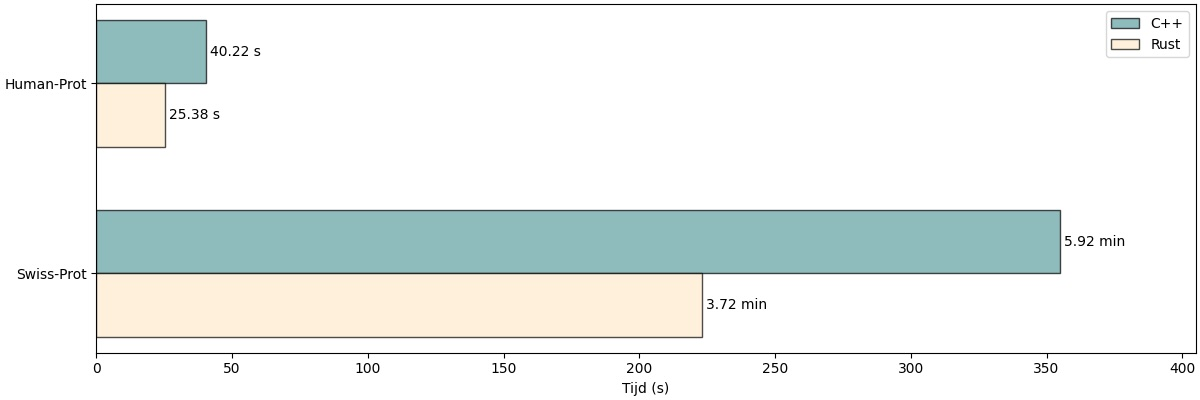
\includegraphics[width=\linewidth]{building_tree_time}}\\[4ex] % [4ex] om wat extra vertical spacing in te voegen

    \subfloat[Maximaal gebruikt geheugen tijdens het opbouwen van de suffixboom.]{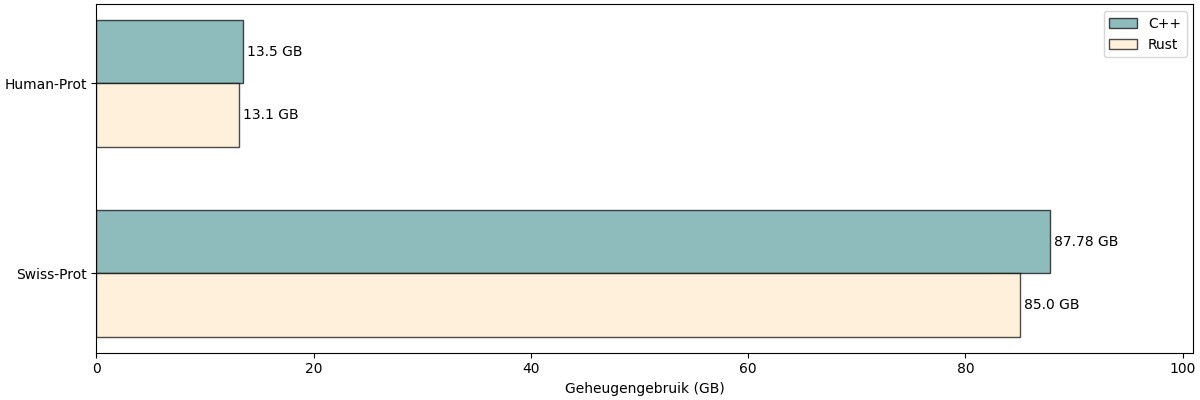
\includegraphics[width=\linewidth]{building_tree_memory}}
    \caption{Vergelijking tusen C++ en Rust voor het opbouwen van de suffixboom a.d.h.v.~het algoritme van Ukkonen. De tijd en het geheugengebruik zijn gemeten met het unix \texttt{time} commando. Als invoerbestand gebruiken we hier de Swiss-Prot of Human-Prot eiwitdatabank.}\label{fig:tree_building}
\end{figure}

Uit deze grafieken vallen 2 duidelijke conclusies te trekken.
\begin{enumerate}
    \item De implementatie in Rust is $\pm$ 33\% sneller
    \item Het geheugenverbruik is erg vergelijkbaar.
    Dit valt te verwachten aangezien beide implementaties 8 bytes nodig hebben per \textit{pointer} en evenveel plaats voorzien voor de kinderen.
    Het kleine verschil valt te verklaren vanwege één veld uit de C++ implementatie dat niet bijgehouden wordt in de Rust implementatie.
    Dit veld is de diepte van de top in de boom.
    Op de enkele plaatsen waar dit nodig is, kan gebruikgemaakt worden van andere variabelen om tot een equivalent resultaat te komen.
\end{enumerate}

\subsubsection{Zoeken}
Bij het zoeken zijn er twee belangrijke toepassingen om de snelheid te meten.
\begin{enumerate}
    \item Zoek totdat we weten of er een match bestaat voor de peptide.
    \item Zoek totdat er een match is, en doorzoek daarna de volledige subboom om alle informatie van de kinderen op te halen.

\end{enumerate}

\paragraph{Zoek een match}
Het meten van de zoektijd tot een match is een belangrijke indicatie van performantie, omdat bepaalde stukken informatie voorberekend kunnen worden voor elke top in de boom.
Hiervoor wordt informatie uit de bladeren tot aan de top van de boom gepropageerd.
In ons geval is dit bijvoorbeeld de LCA\footnote{Lowest Common Ancestor, Laagste Gemeenschappelijke Voorouder. Dit is de meest specifieke top in een boomstructuur (d.w.z.~de top zo diep mogelijk in de boom) die een ouder is van een elke top in de gegeven set van toppen.\label{footnote:lca}} van de taxon IDs.
Dit laat toe om het zoekproces te stoppen zodra er een match is.
De top waarin het zoeken stopt, zal de voorberekende LCA waarin we geïnteresseerd zijn bevatten.
Dit is de LCA van de taxon IDs die horen bij de proteïnen waarvan de gezochte peptide een substring is.
\\ \\
Figuur~\ref{fig:performance_match_tree} toont de nodige tijd om alle peptiden van de gebruikte peptidebestanden éénmalig te zoeken totdat er een (mis)match was voor de peptide.
De grafiek bevat de gemiddelde resultaten van 5000 uitvoeringen, maar zelfs dan bleven de resultaten wat schommelen.
Doordat de te meten tijd zo klein is, kan de kleinste invloed van omgevingsfactoren al voor een zichtbaar verschil zorgen.
Dit kan bv.~een achtergrondproces zijn, maar ook invloed van een andere VM die op de fysieke machine bezig is.
Dit was ook merkbaar tijdens het testen, waar de verschillen tussen twee opeenvolgende uitvoeringen vaak groter waren dan het verschil tussen de C++ en Rust implementatie.
Toch kunnen we besluiten dat de C++ implementatie een beetje performanter is.

\begin{figure}[H]
    \centering
    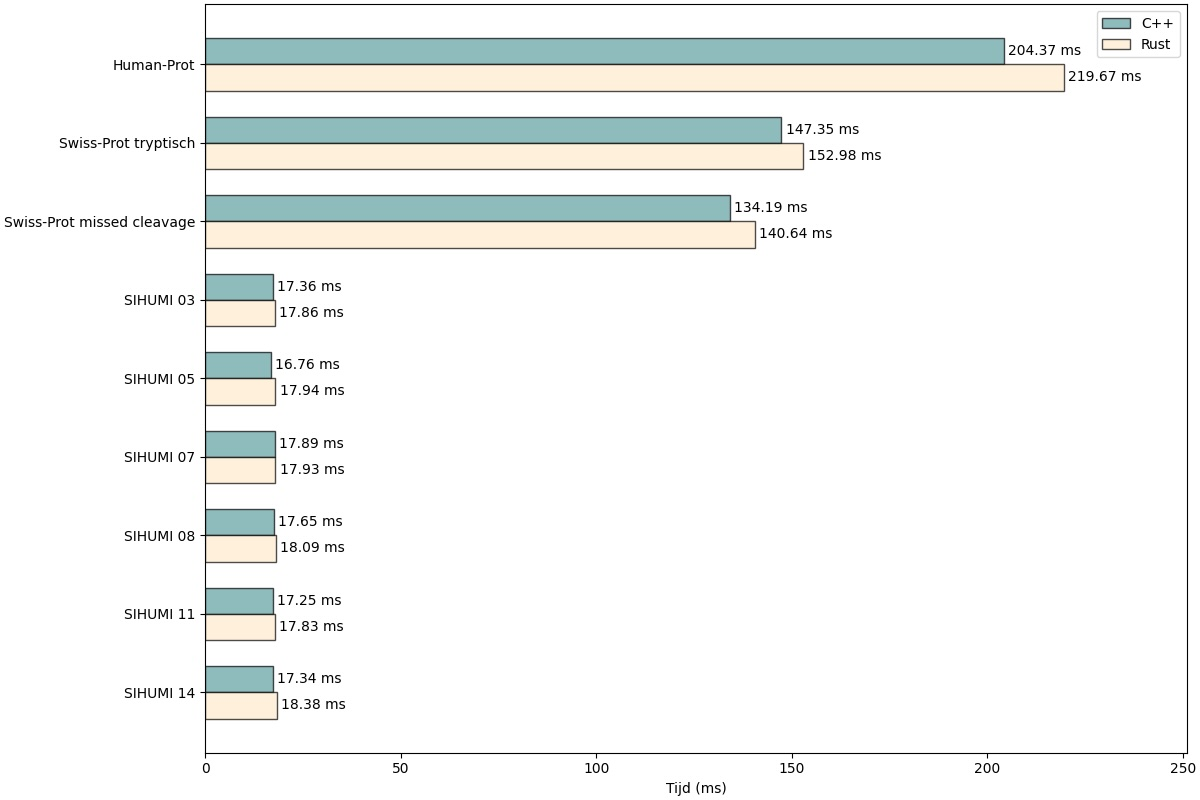
\includegraphics[width=\linewidth]{search_match_performance_tree}
    \caption{Uitvoeringstijd in milliseconden voor het zoeken tot een match voor alle peptidebestanden. Deze resultaten zijn het gemiddelde van 5000 uitvoeringen. Eén iteratie wordt gezien als één maal elke peptide die deel is van het peptidebestanden te zoeken in de suffixboom, en te stoppen wanneer er een (mis)match gevonden is. Het meten van de tijd is gebeurd in de code zelf.}
    \label{fig:performance_match_tree}
\end{figure}

Het verschil met de huidige implementatie van Unipept is aanzienlijk.
Daar duurt het op dit moment 2 minuten en 12 seconden om alle peptiden van het Swiss-Prot peptidebestand zonder \textit{missed cleavages} te zoeken,
en maar liefst 30 minuten en 37 seconden voor het peptidebestand met \textit{missed cleavages}.
Dit is resp.~$\frac{132 000}{152.98} = 857$ en $\frac{1 837 000}{140.64} = 13 000$ keer trager.
Het gebruik van de suffixboom heeft echter ook nadelen ten opzichte van de huidige implementatie.
Deze laatste gebruikt slechts 6.7 GiB geheugen, en dit kan zelfs nog naar beneden.
Dit is ongeveer 13 keer lager dan het geheugengebruik voor de suffixboom implementatie voor Swiss-Prot.

\paragraph{Zoek match en haal informatie over kinderen op}
Indien we alle proteïnen willen vinden waar een peptide mee matcht, dan moeten we de volledige subboom doorzoeken startende van de top waar de match eindigt.
De reden hiervoor is dat alle bladeren in deze subboom de gematchte proteïnen en de bijbehorende taxonomische informatie bevatten.
\\ \\
Figuur~\ref{fig:performance_all-occurrences_tree} bevat een overzicht van de nodige zoektijd voor beide implementaties op alle peptidebestanden.
We zien duidelijk dat er hier een significant verschil is tussen de C++ en Rust implementatie.
Vermoedelijk komt dit door de andere \textit{memory layout} die ontstaat doordat de Rust implementatie 1 grote vector gebruikt, terwijl de C++ implementatie losse toppen gebruikt die verspreid liggen in het geheugen.

\begin{figure}[H]
    \centering
    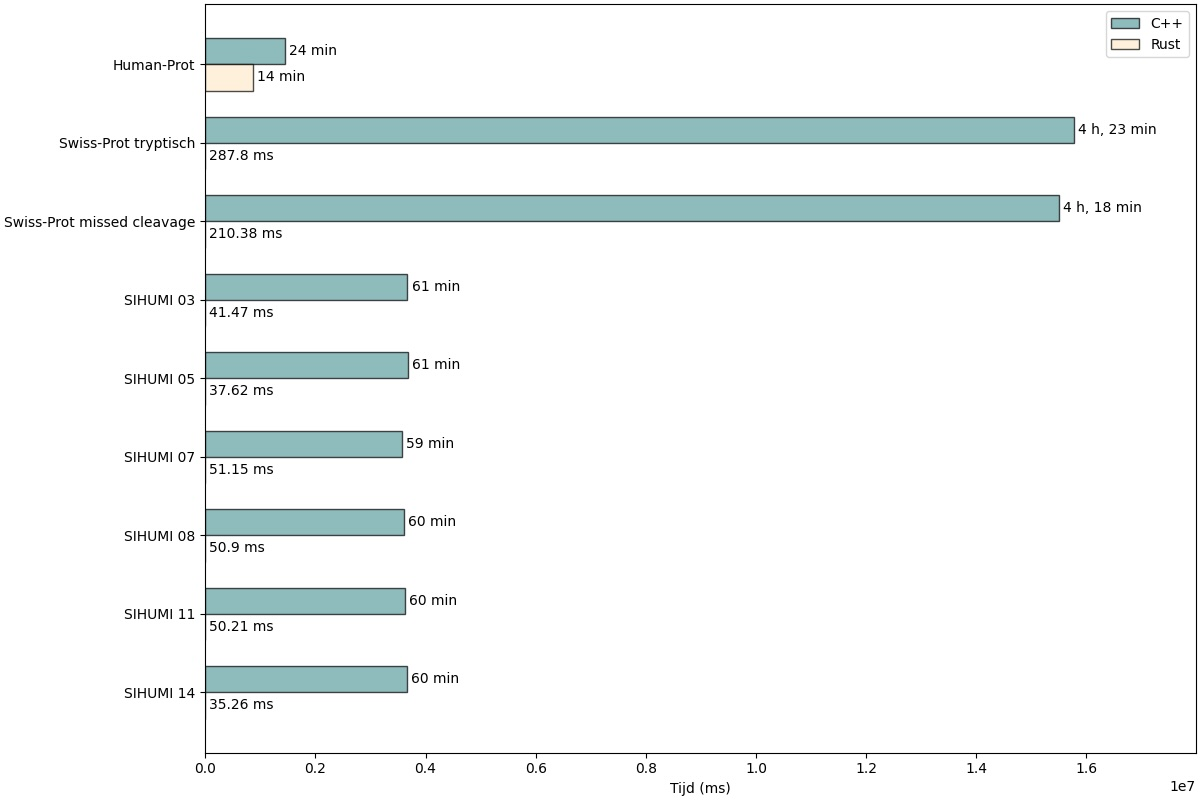
\includegraphics[width=\linewidth]{search_all-occurrences_performance_tree}
    \caption{Uitvoeringstijd inclusief het doorzoeken van de volledige subboom na match voor alle peptidebestanden. Deze resultaten zijn het gemiddelde van 10 uitvoeringen. Eén uitvoering wordt gezien als één keer elke peptide die deel is van het peptidebestand te zoeken in de suffixboom, en bij een match de volledige resterende subboom te doorzoeken. Dit toont de tijd die nodig is om informatie uit de bladeren op te halen voor alle proteïnen waar een peptide substring van is. Het meten van de tijd is gebeurd in de code zelf.}
    \label{fig:performance_all-occurrences_tree}
\end{figure}


\section{Taxon ID aggregatie}\label{sec:taxon-id-aggregatie}
Eén van de belangrijkste analyses die Unipept aanbiedt, is de taxonomische analyse waarbij uitgezocht wordt met welke organismen de peptiden uit een staal overeenkomen.
Aangezien peptiden kunnen matchen met proteïnen uit verschillende organismen, moet er een manier gekozen worden om deze informatie te aggregeren.
Een optie is om een schatting te maken en het organisme met de grootst mogelijke kans te nemen.
Unipept kiest echter een andere aanpak waarbij de informatie conservatief veralgemeend wordt omdat er geen manier is om met zekerheid te zeggen uit welke proteïne de peptide effectief komt.
Dit komt omdat gebruikers enkel een set aan peptides als input geven aan Unipept, niks van extra info dat toelaat om te knippen zonder mogelijks correcte informatie te verliezen.
Anders gezegd: Unipept zal enkel info geven die geldt voor alle gematchte proteïnen.
Eén van deze stukjes informatie is het Taxon ID\@.
Unipept zal niet de lijst van alle mogelijke taxon IDs teruggeven omdat dit twee nadelen heeft.
Ten eerste kan dit een erg grote lijst worden indien de peptide met erg veel proteïnen matcht.
Ten tweede zou dit ook vereisen om altijd de volledige subboom na een match te overlopen.
In plaats daarvan gaan we via voorberekeningen de taxon IDs aggregeren gebruikmakende van de NCBI taxonomy\footnote{Dit is een boomstructuur die de evolutionaire relaties tussen organismen representeert. De laagste gemeenschappelijke voorouder van twee bladeren in deze boom representeert het evolutionair punt waarop deze twee organismen van elkaar afgesplitst zijn. Elke top in deze taxonomische boom heeft een uniek taxon ID, waarbij de root van de boom ID met waarde 1 heeft.} database~\cite{NCBI_original_article, NCBI_update}.
Met andere woorden, we gaan op zoek naar de kleinste gemeenschappelijke voorouder van alle taxon IDs die in de bladeren van de subboom zitten van een bepaalde top.
Hiervoor bestaan verschillende strategieën die al uitgewerkt zijn in UMGAP~\cite{UMGAP_paper, UMGAP_source}, en die hier herbruikbaar waren.
\\ \\
Origineel was het plan om LCA* \footnote{LCA = Lowest Common Ancester, Laagste Gemeenschappelijke Voorouder. De * wijst erop dat dit algoritme een variant is.} te gebruiken als aggregatiestrategie.
Dit is een heuristiek gebaseerd op de LCA\footref{footnote:lca}.
Bij LCA* zoeken we het meest specifieke taxon in de boom die ofwel een ouder of kind is van elke taxon in de boom.
Anders gezegd is dit de LCA van een verzameling taxa, nadat we alle taxa verwijderd hebben die ouder zijn van minstens één taxon in die verzameling~\cite{UMGAP_paper}.
Het voordeel van LCA* ten opzichte van LCA is dat de resulterende data langer exact blijft.
De LCA van een verzameling aan taxon IDs zal namelijk altijd als waarde 1 hebben, dus de root zijn, vanaf één element in de verzameling als root geannoteerd is.
Dit gedrag willen we zo lang mogelijk vermijden.
\\ \\
Om het taxon ID van elke interne top in de boomstructuur efficiënt voor te berekenen was het idee om dit op basis te doen van de directe kinderen van die top.
Hiermee bedoelen we de eerstegraads kinderen.
Deze liggen 1 niveau lager in de boomstructuur, en hebben als ouder allemaal dezelfde top waarvan we het taxon ID willen berekenen.
De andere, tragere, optie is om dit te doen op basis van de bladeren van de subboom van de top.
Door het te doen aan de hand van de directe kinderen van de top kunnen we in één bottom-up sweep van de boom alle taxon IDs berekenen.
Dit bleek echter niet mogelijk in combinatie met LCA* omdat gebruik maken van de directe kinderen een ander resultaat geeft dan gebruik maken van de bladeren van de subboom.
Figuur~\ref{fig:lca*_diff} toont een minimaal voorbeeld uitgewerkt voor beide strategieën.
De licht grijze toppen zijn ingevuld aan de hand van aggregatie, terwijl de zwarte toppen gegeven zijn.

\begin{figure}[H]
    \centering
    \subfloat[LCA* op basis van de bladeren.]{
        \begin{tikzpicture}
            \node [gray] {1}
            child {node [gray] {1}
            child {node {9606}}
            child {node {10566}}}
            child {node {9606}
            };
        \end{tikzpicture}
    }\hspace{0.25\textwidth}%
    \subfloat[LCA* op basis van de kinderen.]{
        \begin{tikzpicture}
            \node [gray] {9606}
            child {node [gray] {1}
            child {node {9606}}
            child {node {10566}}}
            child {node {9606}
            };
        \end{tikzpicture}
    }
    \caption{Minimaal voorbeeld van de 2 aggregatie manieren gebruikmakende van LCA*. De grijze toppen zijn berekend aan de hand van een LCA*, terwijl de zwarte toppen gegeven zijn. In de NCBI databank stelt organisme met ID 10566 het Human papillomavirus voor, organisme met ID 9606 de Homo Sapiens en taxon ID 1 is een representatie van de root van de volledige NCBI taxonomy boomstructuur.}\label{fig:lca*_diff}
\end{figure}

Onderstaande uitleg behandelt de werkwijze voor bovenstaande figuren.
\begin{itemize}
    \item Het toepassen van LCA* voor het berekenen van de top op basis van de bladeren van de boom (\{9606, 10566, 9606\}) heeft als resultaat 1 voor de root van de boom.
    9606 en 10566 zijn geen ouder of kind van elkaar, dus zal LCA* hetzelfde doen als LCA\@.
    De kleinste gemeenschappelijke ouder van deze 2 taxons is 1.
    \item Het toepassen van LCA* op basis van de directe kinderen geeft als resultaat 9606.
    Dit valt simpel te verklaren aangezien de LCA* van de linker subboom 1 is.
    Als we daarna dan de LCA* van \{1, 9606\} nemen wordt 1 verwijderd, aangezien dit een ouder is van 9606.
    De LCA van 9606 is gewoon zichzelf.
\end{itemize}

Het berekenen van de LCA* op de eerste manier is echter niet schaalbaar voor de volledige suffixboom.
Om een idee van grootorde te geven: de suffixboom voor de Swiss-Prot dataset bevat in totaal 328 922 516 toppen, waarvan 206 523 693 bladeren.
\\ \\
Daarom hebben we voorlopig toch voor de standaard LCA aggregatiemanier gekozen.
Deze laat wel toe de toppen op deze efficiëntere manier te aggregeren.
UMGAP biedt 2 implementaties aan om de LCA te berekenen voor een gegeven lijst van taxa.
Gebruikmakende van RMQs\footnote{Range Minimum Queries} of een boomstructuur.
Mijn implementatie maakt gebruik van de RMQ implementatie aangezien deze significant sneller is (8 min 58 sec vs 20 min en 25 sec voor de Swiss-Prot databank) in mijn toepassing.
Tot slot heb ik voor Swiss-Prot ook eens vergeleken hoe groot de behaalde tijdswinst is als we de LCAs aggregeren aan de hand van de directe kinderen, vergeleken met aggregatie op basis van de bladeren.
Bij het aggregeren op basis van de bladeren met de RMQ implementatie was de uitvoeringstijd maar liefst 12 uur, 19 minuten en 16 seconden.
Dit is dus een extreem groot verschil.

\section{Conclusie}\label{sec:conclusie-suffix-bomen}
Het is duidelijk dat suffixbomen erg performant zijn voor het zoeken van willekeurige peptiden in een grote verzameling van proteïnes.
Zelfs als we alle bladeren willen afgaan valt dit mee.
Bovendien is ook het opbouwen van de indexstructuur iets wat relatief snel gaat.
\\ \\
Door de eigen implementatie in Rust, kunnen we ook wat tijd besparen ten opzichte van een equivalente C++ implementatie.
Een deel van de tijdswinst zit in het opbouwen van de boom, maar vooral tijdens het zoeken wanneer informatie uit de bladeren gehaald moet worden.
Vermoedelijk ligt de andere geheugenstructuur hiervoor aan de basis.
\\ \\
Ondanks de veelbelovende resultaten op vlak van snelheid is er een keerzijde aan de medaille.
Het geheugengebruik is zo groot dat we op zoek moeten naar een andere indexstructuur.
Voor de Swiss-Prot databank gaat het geheugenverbruik al boven 85 GB als we ook de taxon IDs voorberekenen, terwijl ons einddoel is om dit toe te passen op de volledige UniprotKB databank.
Dit wil zeggen dat alles nog $\pm$ 500 maal opgeschaald moet worden.
Dit zou echter
Dit zou echter vereisen dat we een server hebben met ongeveer 45 TB aan RAM geheugen.
We hebben echter geen dergelijke machine ter beschikking.
Daarom moeten we op zoek naar andere indexstructuren die minder geheugen vereisen.


    \chapter{Suffix arrays}\label{ch:suffix-arrays}
Een tweede datastructuur die we in meer detail bekijken zijn suffix arrays.
Dit doen we omwille van de lagere geheugenvereisten in vergelijking met suffixbomen.

\section{Wat zijn suffix arrays?}\label{sec:wat-zijn-suffix-arrays?}
Suffix arrays zijn een geheugenefficiëntere voorstelling van suffixbomen.
In plaats van een boomstructuur maken we hier gebruik van een array die de volgnummers van elke suffix in de originele string bevat.
Deze volgnummers worden lexicografisch gesorteerd op basis van de overeenkomstige suffix.
Figuur~\ref{fig:suffixtree_vs_suffixarray} geeft een voorbeeld van een suffixboom en suffix array opgebouwd over de tekst \texttt{acacgt\$}.

\begin{center}
    \texttt{tekst: a|c|a|c|g|t|\$\\index: 0|1|2|3|4|5|6}
\end{center}
\begin{figure}[H]

    \begin{subfigure}[b]{0.6\linewidth}
        \resizebox{\linewidth}{!}{
            \begin{tikzpicture}
            [
                level 1/.style = {sibling distance = 2.5cm},
                level 2/.style = {sibling distance = 1cm}
            ]

                \node[draw, circle] (End2) {}
                child {
                    [fill] circle (2pt)
                    edge from parent node [above] {6,7}
                }
                child {
                    node[draw, circle] (Start1) {}
                    child {
                        [fill] circle (2pt)
                        edge from parent node [left] {2,7}
                    }
                    child {
                        [fill] circle (2pt)
                        edge from parent node [right] {4,7}
                    }
                    edge from parent node [below] {0,2}
                }
                child {
                    node[draw, circle] (End1) {}
                    child {
                        [fill] circle (2pt)
                        edge from parent node [left] {2,7}
                    }
                    child {
                        [fill] circle (2pt)
                        edge from parent node [right] {4,7}
                    }
                    edge from parent node [left] {1,2}
                }
                child {
                    [fill] circle (2pt)
                    edge from parent node [below] {4,7}
                }
                child {
                    [fill] circle (2pt)
                    edge from parent node [above] {5,7}
                }
                ;
                \draw[dashed, ->] (Start1) to[out=-20,in=200] (End1);
                \draw[dashed, ->] (End1) to[out=60,in=-60] (End2);
            \end{tikzpicture}
        }
        \caption{Suffixboom}
    \end{subfigure}
    \begin{subfigure}[b]{0.4\linewidth}
        \centering
        \begin{tikzpicture}[thick,scale=.6]
            \draw (0,0) grid (7,1);
            \path (.5,.5) node{$6$} foreach \i in {0,2,1,3,4,5} {++(1,0) node{$\i$}};
        \end{tikzpicture}
        \vspace{3em} % vertically center the array a bit
        \caption{Suffix array}
    \end{subfigure}

    \caption{Suffixboom en suffix array voor de string \texttt{acacgt\$}.}\label{fig:suffixtree_vs_suffixarray}
\end{figure}

Wanneer we de bladeren van de suffixboom van links naar rechts bekijken dan valt te zien dat dit overeen komt met de suffix array.
Dit is dan ook de link tussen deze twee datastructuren.
Onmiddellijk valt ook te zien dat een suffix array minder data bevat.
De interne knopen en suffix links uit de suffixboom ontbreken.
Indien deze informatie ook nodig is kan gebruik maakt worden van zogenaamde Enhanced Suffix Arrays (ESAs).
Hierbij worden naast de suffix array nog drie extra tabellen bijgehouden.
Deze worden de LCP, Child en suffix link table genoemd.


\section{Complexiteit}\label{sec:complexiteit}
Naïef kan het opbouwen van een suffix array aan de hand van traditionele sorteeralgoritmes zoals merge sort~\cite{mergeSort} in $O(n \log n)$ tijd en $O(n^2)$ geheugen.
Hierbij is $n$ de lengte van de tekst.
Ondertussen bestaan er echter verschillende algoritmes die een tijdscomplexiteit van $O(n)$ bereiken~\cite{sais, ko_alura, radixSA, dark_archon, libdivsufsort}.
Bovendien vereisen deze veel minder geheugen dan een equivalente suffixboom.
Sommige implementaties vereisen slechts $5n + O(1)$ geheugen~\cite{dark_archon, libdivsufsort}.


\section{Bestaande implementaties}\label{sec:bestaande-implementaties}
Aangezien er meerdere sterk geoptimaliseerde implementaties bestaan voor het opbouwen van een suffix array vergelijken we eerst de performantie van deze implementaties.
Hieruit kunnen we nadien een algoritmes en implementaties selecteren die geheugenefficiënt zijn.
Tabel~\ref{tab:sa_building} bevat een overzicht van verschillende algoritmes waarbij voor sommige algoritmes verschillende implementaties getest zijn.

\begin{table}[H]
    \begin{minipage}{\linewidth}
        \centering
            \begin{tabular}{l l S[table-format=-2.2] S[table-format=-2.2] S[table-format=-1.2] S[table-format=-1.2]}
                Algoritme & Programmeertaal & \multicolumn{2}{c}{Tijd (in sec)} & \multicolumn{2}{c}{Geheugen (in GB)} \\
                \hline\hline
                &                      & {32 bit} & {64 bit} & {32 bit} & {64 bit} \\
                \cline{3-6}
                libdivsufsort\footnote{\url{https://github.com/y-256/libdivsufsort}}                                       & C                    & 15.01    & 15.97    & 1.03     & 1.86     \\
                libdivsufsort\footnote{\url{https://github.com/baku4/libdivsufsort-rs}}                                    & Rust + bindings to C & 16.00    & 15.52    & 1.03     & 1.86     \\
                libdivsufsort\footnote{\url{https://github.com/fasterthanlime/stringsearch/tree/master/crates/divsufsort}}  & Rust                 & 20.23    & {-}      & 1.03     & {-}      \\
                dark archon a4\footnote{\url{https://github.com/kvark/dark-archon}}                                        & C                    & 39.34    & {-}      & 1.09     & {-}      \\
                libsais\footnote{\url{https://github.com/IlyaGrebnov/libsais}}                                             & C                    & 6.38     & 6.46     & 1.03     & 1.86     \\
                SA-IS\footnote{\url{https://github.com/Tascate/Suffix-Arrays-in-CPP}}                                      & C++                  & 24.39    & {-}      & 3.80     & {-}      \\
                SA-IS\footnote{\url{https://github.com/sile/sais}}                                                         & C++                  & 18.73    & {-}      & 1.46     & {-}      \\
                radixSA\footnote{\url{https://github.com/mariusmni/radixSA64}}                                             & C++                  & 9.74     & 11.26    & 2.11     & 3.52     \\
                \hline
            \end{tabular}
        \caption{Uitvoeringstijden en maximaal geheugenverbruik voor het opbouwen van een suffix array aan de hand van verschillende algoritmes voor de Swiss-Prot eiwitdatabank.
        Indien er een 32 bit en 64 bit integer implementatie beschikbaar was werden deze allebei getest. Een - staat voor niet getest. Deze testen werden lokaal uitgevoerd op een M1 Pro MacBook Pro. De specificaties hiervan zijn terug te vinden in tabel~\ref{tab:macbook_hardware}.}
        \label{tab:sa_building}
    \end{minipage}
\end{table}

We kunnen concluderen dat libsais duidelijk de snelste implementatie is om Swiss-Prot te indexeren.
Samen met libdivsufsort gebruikt het de kleinste hoeveelheid geheugen, wat libdivsufsort ook interessant maakt.
Een ander voordeel dat libsais en libdivsufsort hebben (naast hun minimale geheugenverbruik) is dat ze allebei een 64 bit integer implementatie hebben.
Dit is belangrijk voor het indexeren van UniprotKB omdat de totale tekst langer is dan de maximale 32 bit integer.
Dit zorgt ervoor dat alle 32 bit integer implementaties onbruikbaar zijn voor dit einddoel.
Tot slot valt ook te zien dat het verschil tussen de C versie en Rust versie die bindings heeft naar de C code klein is.
De overhead van het oproepen van de C code uit Rust is dus minimaal.

\section{Toepassen van suffix arrays op een eiwitdatabank}\label{sec:toepassen-van-suffix-arrays-op-een-eiwitdatabank}
Het moeilijkste stuk van onze probleemstelling is het opbouwen van de suffix array.
Dit stuk kunnen we oplossen aan de hand van de algoritmes uit sectie~\ref{sec:bestaande-implementaties}.
Eens we die suffix array opgebouwd hebben blijft er echter nog een stuk van ons probleem over.
Om te beginnen moeten we nog een mapping maken van de gevonden suffixen naar het bijbehorende eiwit.
Op basis van dit eiwit wordt daarna de LCA gezocht.

\subsection{Bouwen van de suffix array}\label{subsec:bouwen-van-de-suffix-array}
Zoals in de inleiding van sectie~\ref{sec:probleemstelling} willen we gebruik maken van Rust vanwege de combinatie van \textit{memory safety} en hoge performantie.
We willen echter gebruik maken van de al bestaande geoptimaliseerde implementaties van algoritmes om een suffix array op te bouwen.
Om beide doelen te bereiken maken we gebruik van interoperabiliteit tussen Rust en C/C++.
Zo bestaan er al bindings\footnote{\url{https://crates.io/crates/libdivsufsort-rs}} van Rust naar de originele implementatie van libdivsufsort\cite{libdivsufsort} (in C).
Ook al blijkt uit het testen dat dit algoritme voor het opbouwen van de indexstructuur over een kleinere eiwitdatabank niet het snelste is, het geheugengebruik is wel minimaal.
Dit laat toe om te experimenteren met het opbouwen van een SA zonder al te veel extra werk, en al onmiddellijk te zien hoe het geheugengebruik evolueert.
\\ \\
Later hebben we beslist om zelf nog een simple Rust wrapper te schrijven rond de libsais C code.
Dit gebruik makende van het \texttt{bindgen}\footnote{\url{https://crates.io/crates/bindgen}} crate.
Op deze manier is het ook mogelijk om gebruik te maken van de snellere libsais algoritme eens we wisten dat SAs een efficiënte en schaalbare oplossing waren voor de probleemstelling.
\\ \\
Het nadeel van het gebruiken van deze bindings naar C code is dat het oproepen van de effectieve C code gebeurt in een \texttt{unsafe} blok.
Hierbij is het dus mogelijk dat er geheugenfouten in het programma sluipen.
Dit risico is echter miniem aangezien dit bestaande, geteste bibliotheken zijn.
Bovendien zijn we ook zeker dat eventuele geheugenfouten enkel hierdoor kunnen ontstaan.
Dit is dus een afweging tussen optimale performantie (waarbij we het wiel niet hoeven heruit te vinden), en garantie van \textit{memory safety}.

\subsection{Mapping van suffix naar proteïne}\label{subsec:mapping-van-suffix-naar-proteine}
Bepalen welke proteïne hoort bij een bepaalde suffix kan op twee manieren.
Een eerste optie is om expliciet voor elke suffix bij te houden bij welke proteïne die hoort.
Dit kan aan de hand van een array die even lang is als het aantal suffixen.
Het voordeel van deze aanpak is dat het vinden van de bijbehorende proteïne in $O(1)$ tijd kan, hiervoor is echter wel $O(m)$ geheugen nodig, met $m$ de lengte van de totale tekst.
\\ \\
De tweede optie is om enkel de eerste of laatste suffix per proteïne bij te houden.
Het voordeel van deze aanpak is dat er minder geheugen nodig is, meer precies $O(n)$ geheugen met $n$ het aantal proteïnen.
Het nadeel is dan weer dat het vinden van de bijbehorende proteïne trager is.
Dit neemt $O(\log n)$ tijd in beslag aan de hand van binair zoeken.
Hierbij is $n$ het aantal proteïnes.
\\ \\
In Figuur~\ref{fig:dense_vs_sparse} wordt de uitvoeringstijd voor beide implementaties vergeleken.
Standaard (en in alle komende testen) zullen wij gebruik maken van de sparse versie aangezien de performantie impact in de praktijk beperkt is, en er een significante hoeveelheid geheugengebruik uitgespaard kan worden.
Het grote verschil bij het Human-Prot peptidebestand valt te verklaren vanwege het extreem hoog aantal matches dat daar te vinden is voor de korte peptides.
In de praktijk zullen we dit maximaal aantal matches echter limiteren (zie sectie~\ref{subsec:maximaal-aantal-matches}).
Dit zal op zijn beurt ook de overhead van de sparse mapping beperkt houden.
\begin{figure}[H]
    \centering
    \subfloat[Tijd nodig om alle matches te zoeken.]{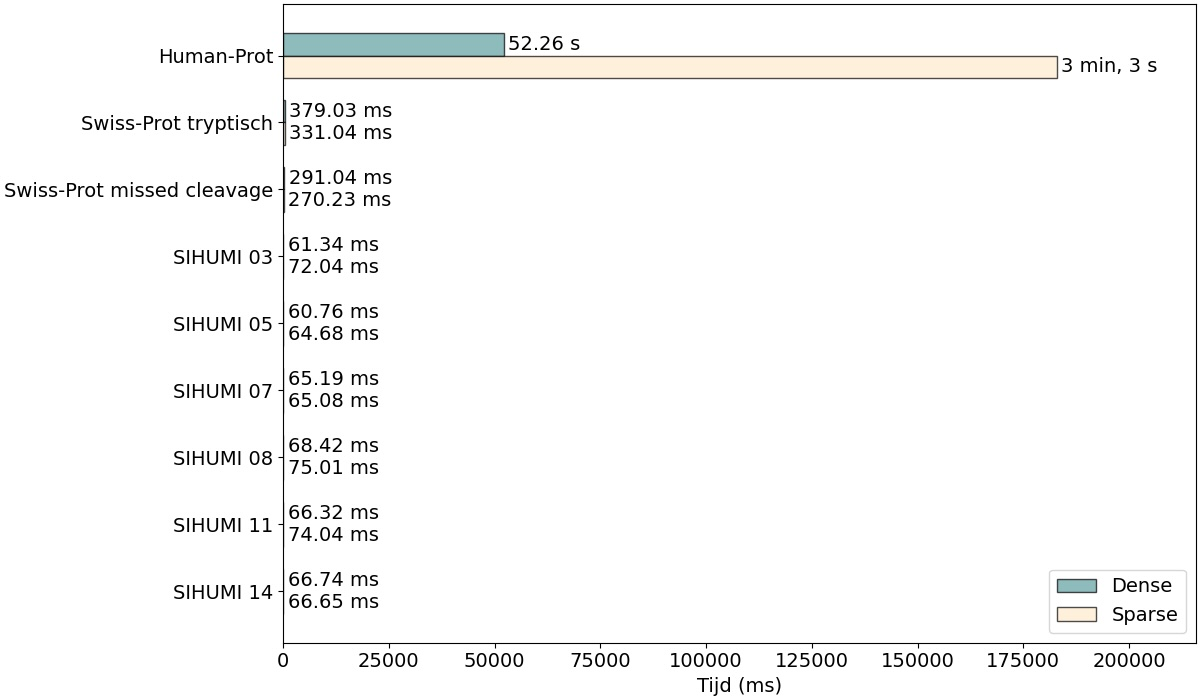
\includegraphics[width=\linewidth]{dense_vs_sparse_time}}\\[4ex] % [4ex] om wat extra vertical spacing in te voegen

    \subfloat[Maximaal gebruikt geheugen tijdens het zoeken naar alle matches.]{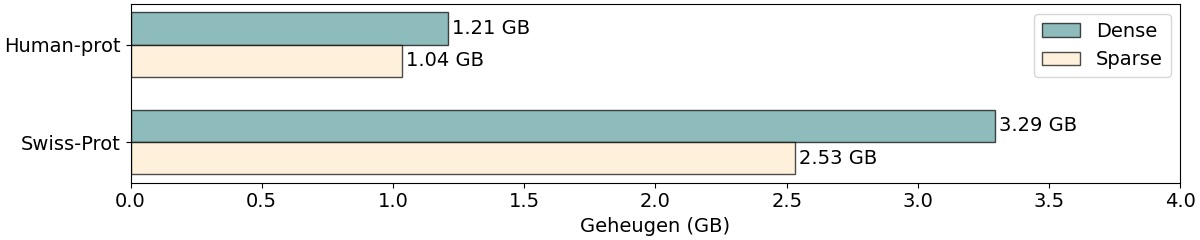
\includegraphics[width=\linewidth]{dense_vs_sparse_memory}}
    \caption{Zoektijd en geheugengebruik bij het gebruik bij een dense of sparse mapping van de suffixen naar de proteïnes.}\label{fig:dense_vs_sparse}
\end{figure}

\subsection{Berekenen van de LCA}\label{subsec:berekenen-van-de-lca}
Zoals eerder vermeld bevat een suffix array geen informatie over de interne toppen die voorkomen bij een suffixboom.
Dit zorgt ervoor dat het niet mogelijk is om op basis hiervan de LCA van de organismen voor te berekenen voor al deze interne toppen.
In de plaats moet dit nu \textit{on the fly} gebeuren tijdens het zoekproces zelf.
Aangezien dit nu niet meer op voorhand berekend wordt, is er geen reden om LCA te verkiezen boven LCA*.
LCA* was namelijk onze eerste keuze, maar bij suffixbomen zijn we daarvan afgestapt om het voorberekenen efficiënter te maken.

% TODO: we kunnen ook gebruik maken van enhanded suffix arrays en dat dan wel proberen doen, maar haalbaarheid daarvan is nog uit te zoeken.


\section{Sparse en compressed suffix arrays}\label{sec:sparse-en-compressed-suffix-arrays}
Om het geheugenverbruik van suffix arrays verder te verkleinen kan er gebruik gemaakt worden van sparse of compressed suffix arrays.
In principe doen ze allebei hetzelfde, er wordt namelijk slechts een stuk van de originele suffix array bijgehouden.
Het verschil zit in welk stuk bijgehouden wordt.
\\ \\
Sparse suffix arrays (SSAs) bouwen een suffix array op basis van elke k-de suffix van de input tekst.
Bij compressed suffix arrays (CSAs) wordt daarentegen slechts elke k-de waarde van de SA bijgehouden.
Voor beide opties is de populairste manier om ze op te bouwen aan de hand van sampling op de volledige SA\@.
Hierdoor blijft het maximale geheugenverbruik tijdens het opbouwen identiek aan het gebruik van de volledige SA\@.
Dit is net het punt waar wij ons geheugenverbruik verder willen verlagen.
Gelukkig heeft het gebruik hiervan nog altijd het voordeel dat de uiteindelijke machine die de index zal hosten lagere geheugenvereisten zal hebben.
\\ \\
Het samplen is de meest gebruikte methode tot op vandaag vanwege de bestaande sterk geoptimaliseerde implementaties van de klassieke SA constructie algoritmes.
Bij sparse suffix arrays is het beste algoritme qua tijdscomplexiteit tot nu toe een Monte Carlo algoritme dat $O(n)$ tijd en $O(b)$ geheugen nodig heeft en een Las Vegas algoritme dat $O(n \sqrt{\log b})$ tijd en $O(b)$ geheugen verbruikt.
Hierbij is $n$ de lengte van de tekst, en $b$ het aantal effectief gebruikte suffixes in de sparse SA~\cite{building_sparse_sa}.
Van het Monte-Carlo algoritme is er een bestaand implementatie\footnote{\url{https://github.com/lorrainea/SSA/tree/main/MA}}.
Wanneer we aan de hand hiervan een SSA met sparseness factor 3 voor Swiss-Prot opbouwen blijkt dit niet alleen trager ($\pm$ 10 minuten) te zijn.
Ook het geheugengebruik ligt merkelijk hoger ($\pm$ 10 GB).
Terwijl we slechts een tiental seconden nodig hebben om de standaard SA op te bouwen in combinatie met 1.8 GB RAM\@.
Voor compressed suffix arrays bestaat er een algoritme dat een tijdscomplexiteit van $o(n)$ heeft in combinatie met $O(n \log \sigma)$ bits aan geheugen~\cite{building_compressed_sa}.
Hierbij is $n$ de tekstlengte en $\sigma$ de alfabetgrootte.
\\ \\
Het grootste nadeel aan deze algoritmes in context van deze thesis is dat er nog geen (sterk geoptimaliseerde) implementaties bestaan.
Bovendien zal de factor van ingevoegde sparseness in ons geval altijd vrij klein zijn om de zoektijden beperkt te houden (aangezien we werken met een erg grote dataset en vrij korte strings).
Indien we dus een implementatie hebben om rechtstreeks een CSA of SSA te bouwen, maar met een grotere constante qua geheugengebruik zal vanwege de kleine sparseness factor de winst snel verloren gaan.
Bovendien laat een CSA niet toe om rechtstreeks gebruik makende van de CSA te zoeken, er zijn nog extra hulp structuren nodig, wat opnieuw extra geheugen vraagt. % TODO: vraag eens aan peter hoe dat werkt, of dubbel check nog eens online, maar is weinig van te vinden
Daarom zijn SSAs interessanter in ons geval aangezien wij matches willen zoeken.
Deze laten toe om enkel met behulp van de tekst en de SSA te zoeken.

\subsection{Zoeken in sparse suffix arrays}\label{subsec:zoeken-in-sparse-suffix-arrays}
Het zoeken in een SSA is erg gelijkaardig aan het zoeken in een volledige SA\@.
Een belangrijke restrictie is echter dat in de SSA geen strings gezocht kunnen worden die kleiner dan of gelijk zijn aan de sparseness factor.
Bovendien heeft deze sparseness factor ook een erg belangrijke impact op de zoekperformantie.
Bij het zoeken met sparseness factor $k$ moeten we namelijk alle suffixen zoeken die matchen met de gezochte string waarbij de eerste $p \in [0, k-1]$ tekens overgeslagen worden.
Voor elke matchende suffix (stel dat dit suffix $s$ is) moet daarna gecontroleerd worden als de overgeslagen prefix van $p$ tekens matcht met de $p$ tekens die op posities $[s - p, p[$ in de geïndexeerde tekst staan.
Als dit zo is, dan matcht suffix $s - p$ met de gezochte string.
Om alles iets duidelijker te maken volgt een klein voorbeeld waarin we de peptide \texttt{acg} in de tekst \texttt{acacgt\$} zoeken.
De index die gebruikt wordt om te zoeken is een SSA met sparseness factor 3.
Deze valt terug te vinden in figuur~\ref{fig:sparse_sa}.

\begin{center}
    \texttt{tekst: a|c|a|c|g|t|\$\\index: 0|1|2|3|4|5|6}
\end{center}
\begin{figure}[H]
    \hfill
    \begin{subfigure}[t]{0.45\linewidth}
        \centering
        \begin{tikzpicture}[thick,scale=.6]
            \draw (0,0) grid (7,1);
            \path (.5,.5) node{$6$} foreach \i in {0,2,1,3,4,5} {++(1,0) node{$\i$}};
        \end{tikzpicture}
        \caption{Suffix array}
    \end{subfigure}
    \hfill
    \begin{subfigure}[t]{0.45\linewidth}
        \centering
        \begin{tikzpicture}[thick,scale=.6]
            \draw (0,0) grid (3,1);
            \path (.5,.5) node{$6$} foreach \i in {0,3} {++(1,0) node{$\i$}};
        \end{tikzpicture}
        \caption{Sparse suffix array met sparseness factor 3.}
    \end{subfigure}
    \hfill
    \caption{SA en SSA voor de tekst \texttt{acacgt\$}.}
    \label{fig:sparse_sa}
\end{figure}

\begin{enumerate}
    \item Sla 0 tekens over.
    Zoek \texttt{acg} in de SSA\@.
    We vinden geen matches.
    \item Sla 1 teken over.
    Dit wil zeggen dat we \texttt{cg} zoeken in de SSA\@.
    Dit levert een match op met suffix 3 (op index 1 in de SSA).
    \begin{enumerate}
        \item Controleer als de suffix die deels gematcht is ook volledig matcht met onze zoekstring.
        Dit wil zeggen dat we de overgeslagen prefix van $p = 1$ tekens (in dit geval de letter \texttt{a}) moeten kunnen matchen met de eerste $p$ tekens van suffix $3 - 1 = 2$.
        \item We zien dat het eerste teken van suffix 2 inderdaad een \texttt{a} is.
        Hiervoor is de SA zelf niet nodig, dit kan rechtstreeks via tekst gecontroleerd worden aan de hand van $p$ karakters die vergeleken moeten worden.
        Suffix 2 is dus een match voor de zoekstring \texttt{acg}.
    \end{enumerate}
    \item Sla 2 tekens over.
    Zoek \texttt{g} in de SSA\@.
    We vinden geen matches.
    \item We concluderen dat enkel suffix 2 matcht met de gezochte string \textit{acg}.
\end{enumerate}

\subsubsection{Performantie en indexgrootte}
Zoals eerder vermeldt heeft de sparseness factor een invloed op zowel de zoekperformantie als de indexgrootte.
Zo zal een grotere sparseness factor niet alleen meer iteraties vragen.
Deze extra iteraties zullen er op hun beurt ook voor zorgen dat er kortere stukken in de SSA gezocht zullen worden, die in het algemeen meer matches zullen opleveren.
Voor al deze matches moeten we controleren als de tekens die ervoor komen matchen met de overgeslagen prefix.
Figuur~\ref{fig:search_sparseness}~(a) visualiseert de impact hiervan op de zoektijd van het Swiss-Prot peptidebestand met en zonder \textit{missed cleavages}.
Deze bestanden worden hiervoor gebruikt omdat de kortste sequentie die ze bevatten 5 aminozuren lang is.
Hierdoor blijft voor het gebruikte interval nog steeds elke peptide zoekbaar.
Zoals eerder al aangehaald kunnen peptides die minder lang zijn dan de sparseness factor niet meer gezocht worden.
Indien we het peptidebestand voor Human-Prot zouden gebruiken zou de evolutie van de zoektijd minder representatief zijn.
Dit omdat er een deel van de peptides korter zijn dan 5 aminozuren lang, deze zouden dus overgeslagen moeten worden.
\\
\begin{figure}[H]
    \centering
    \subfloat[Zoektijd voor het Swiss-Prot peptidebestand met en zonder missed cleavages in een sparse suffix array gebouwd aan de hand van de Swiss-Prot eiwitdatabank.]{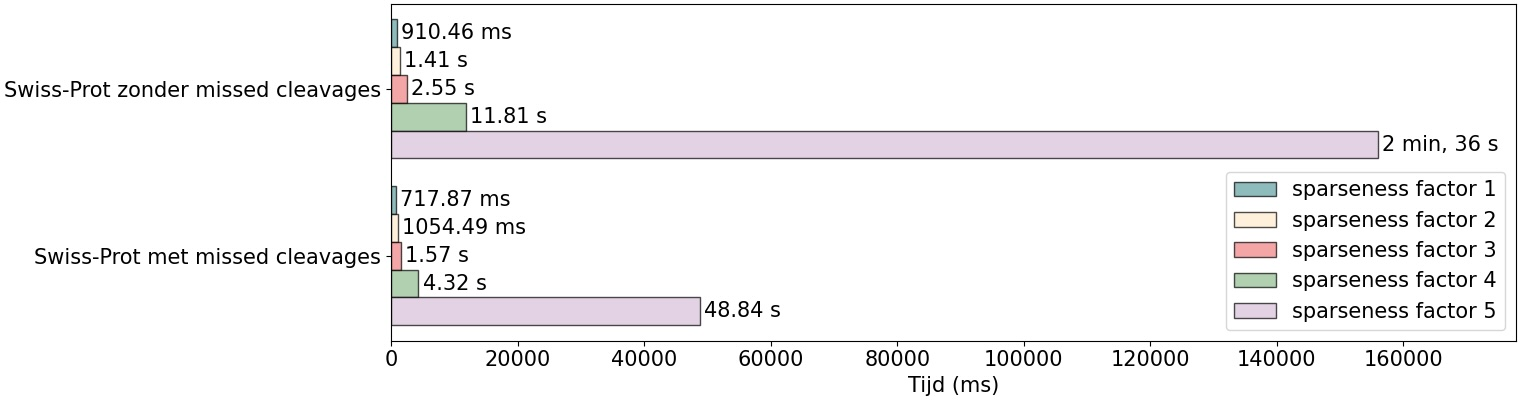
\includegraphics[width=\linewidth]{swissprot_searchtime_sparseness}}\\[4ex] % [4ex] om wat extra vertical spacing in te voegen

    \subfloat[Grootte van de volledige index en SSA voor de Swiss-Prot databank gebruik makende van verschillende sparseness factors.]{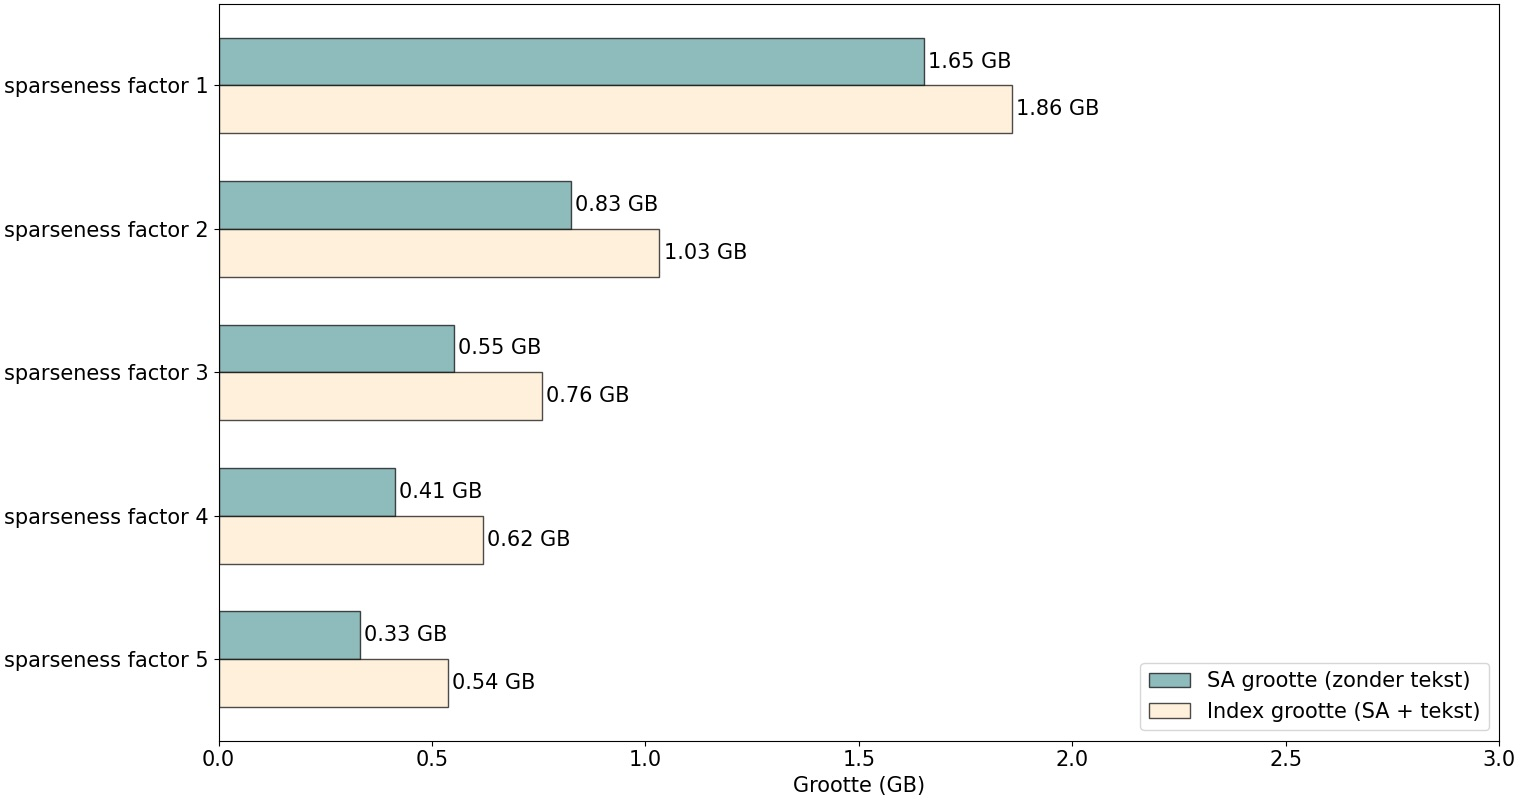
\includegraphics[width=0.8\linewidth]{index_size_SSA}}
    \caption{Zoektijd en indexgrootte voor Swiss-Prot.}\label{fig:search_sparseness}
\end{figure}

De zoektijd explodeert wanneer we de sparseness factor verhogen omdat er een deel van de gezochte peptides bestaat uit 5 aminozuren.
Wanneer we deze proberen zoeken in een SSA een sparseness factor 5, zoeken we eigenlijk enkel één letter in de SSA (de laatste van de peptide).
Deze zal erg veel matches opleveren, en op zijn beurt erg veel werk vragen om alle prefixen hiervan te controleren.
\\ \\
Anderzijds zal het verhogen van de sparseness factor de indexgrootte verkleinen.
Hierbij is het belangrijk dat enkel de SA mee verkleint.
Er blijft altijd een vaste hoeveelheid geheugen nodig om de tekst zelf nog op te slaan.
Figuur~\ref{fig:search_sparseness}~(b) toont dit.
Er is duidelijk te zien dat voor dit geval de overgang van sparseness factor 4 naar 5 erg weinig winst heeft in opslag, maar een grote impact heeft op de performantie.
\\ \\
Er zijn dus twee erg belangrijke bevindingen over sparse suffix arrays, en de manier waarop wij ze opbouwen.
\begin{enumerate}
    \item Probeer de sparseness factor zo laag mogelijk te houden, zo blijft ook de zoektijd voor kortere peptiden beperkt.
    \item Het maximale geheugenverbruik blijft constant onafhankelijk van de sparseness factor.
    De hoeveelheid geheugen om ze nadien te gebruiken kunnen we wel verkleinen, hierdoor kan de index op lichtere machines gebruikt worden na het opbouwen.
\end{enumerate}

Dit impliceert dat we de factor enkel moeten verhogen om het geheugenverbruik te beperken bij een al opgebouwde indexstructuur.
Dit is vooral van toepassing voor UniProtKB waar het nuttig is om kort een krachtige machine te gebruiken die de SA bouwt, waarna een minder krachtige machine de SSA host.
In het perfecte geval wordt de sparseness factor zo gekozen zodat de SSA samen met de tekst net in het RAM geheugen past van deze minder krachtige machine.

\section{Parallellisatie}\label{sec:parallellisatie}
Om het zoeken nog verder te versnellen kan gebruik gemaakt worden van parallellisatie.
We hebben namelijk een groot aantal peptides waarvoor we elke keer dezelfde statische indexstructuur moeten doorzoeken.
Rust maakt dit proces vrij simpel omdat het \textit{ownership} systeem dataraces voorkomt (behalve wanneer gebruik gemaakt wordt van \textit{unsafe} code of het \textit{interior mutability} patroon)\cite{rust_data_races}.
Om een datatype te gebruiken in combinatie met multithreading moet deze de \texttt{Sync} en \texttt{Send} trait implementeren.
Deze traits worden door het typesysteem automatisch afgeleid.
Als namelijk alle componenten van een type aan de \texttt{Sync} en \texttt{Send} trait voldoen, dan voldoet je nieuwe type ook automatisch.
\\ \\
Uiteindelijk hebben we twee geparallelliseerde implementaties gemaakt.
In de eerste wordt alles volledig zelf beheerd.
Hierbij verdelen we zelf welke data naar welke thread gaat, worden de threads manueel opgestart en sluiten we ze ook zelf af.
In de tweede implementatie wordt gebruik gemaakt van de Rayon crate\cite{rayon}.
Deze laat toe om op een simpele manier een sequentiële lus over een variabele te parallelliseren.
In ons geval was het omzetten van een sequentiële implementatie (nadat alle types voldeden aan de \texttt{Sync} en \texttt{Send} trait) zo simpel als het vervangen van \texttt{.iter()} door \texttt{.par\_iter()}.
Ook in deze implementatie is het mogelijk om manueel een specifiek aantal threads te kiezen.
Standaard gebruikt Rayen het aantal beschikbare logische cores op de machine, maar het instellen van een ander aantal kan aan de hand van één lijntje code.

\begin{minted}{Rust}
// Sequentieel
let results = peptides
    .iter()
    .map(|peptide| search_peptide(peptide))
    .collect();

// Parallel
let results = peptides
    .par_iter()
    .map(|peptide| search_peptide(peptide))
    .collect();
\end{minted}

\subsection{Manueel threaden vs Rayon}\label{subsec:manueel-threaden-vs-rayon}
Aangezien we twee verschillende implementaties hebben is het interessant om na te gaan hoe deze allebei presteren.
Figuur~\ref{fig:threading_default_vs_rayon} toont de evolutie van de zoektijden voor een verschillend aantal threads.
We zien duidelijk dat de versie die gebruikt maakt van Rayon net iets sneller is en dat beide implementaties $\pm$ lineair schalen.
De schaling is niet perfect 1--1 ten opzichte van het aantal threads omdat het inlezen en uitschrijven van de output sequentieel blijft.
Het verschil in uitvoeringstijd valt mogelijks te verklaren aan de manier waarop de data verdeeld wordt over de threads in combinatie met een efficiëntere manier om de resultaten uit de threads te verwerken.
In de eigen implementatie kreeg elke thread simpelweg $\frac{1}{x}$ van alle peptides toegekend, met $x$ het aantal threads.
De resultaten moeten daarna aan de hand van enkele stappen uit de thread-scope gehaald worden zodat deze terug beschikbaar zijn voor de rest van het programma.
Rayon maakt gebruik van een ingewikkelder systeem aan de hand van \textit{work stealing}\cite{rayon_stealing} om de data over de threads te verdelen.
Verder is het ophalen van de resultaten ook veel simpeler.
Deze worden rechtstreeks ter beschikking gesteld alsof er geen parallellisme was.

\begin{figure}[H]
    \centering
    \subfloat[Absolute uitvoeringstijd voor een verschillend aantal cores.]{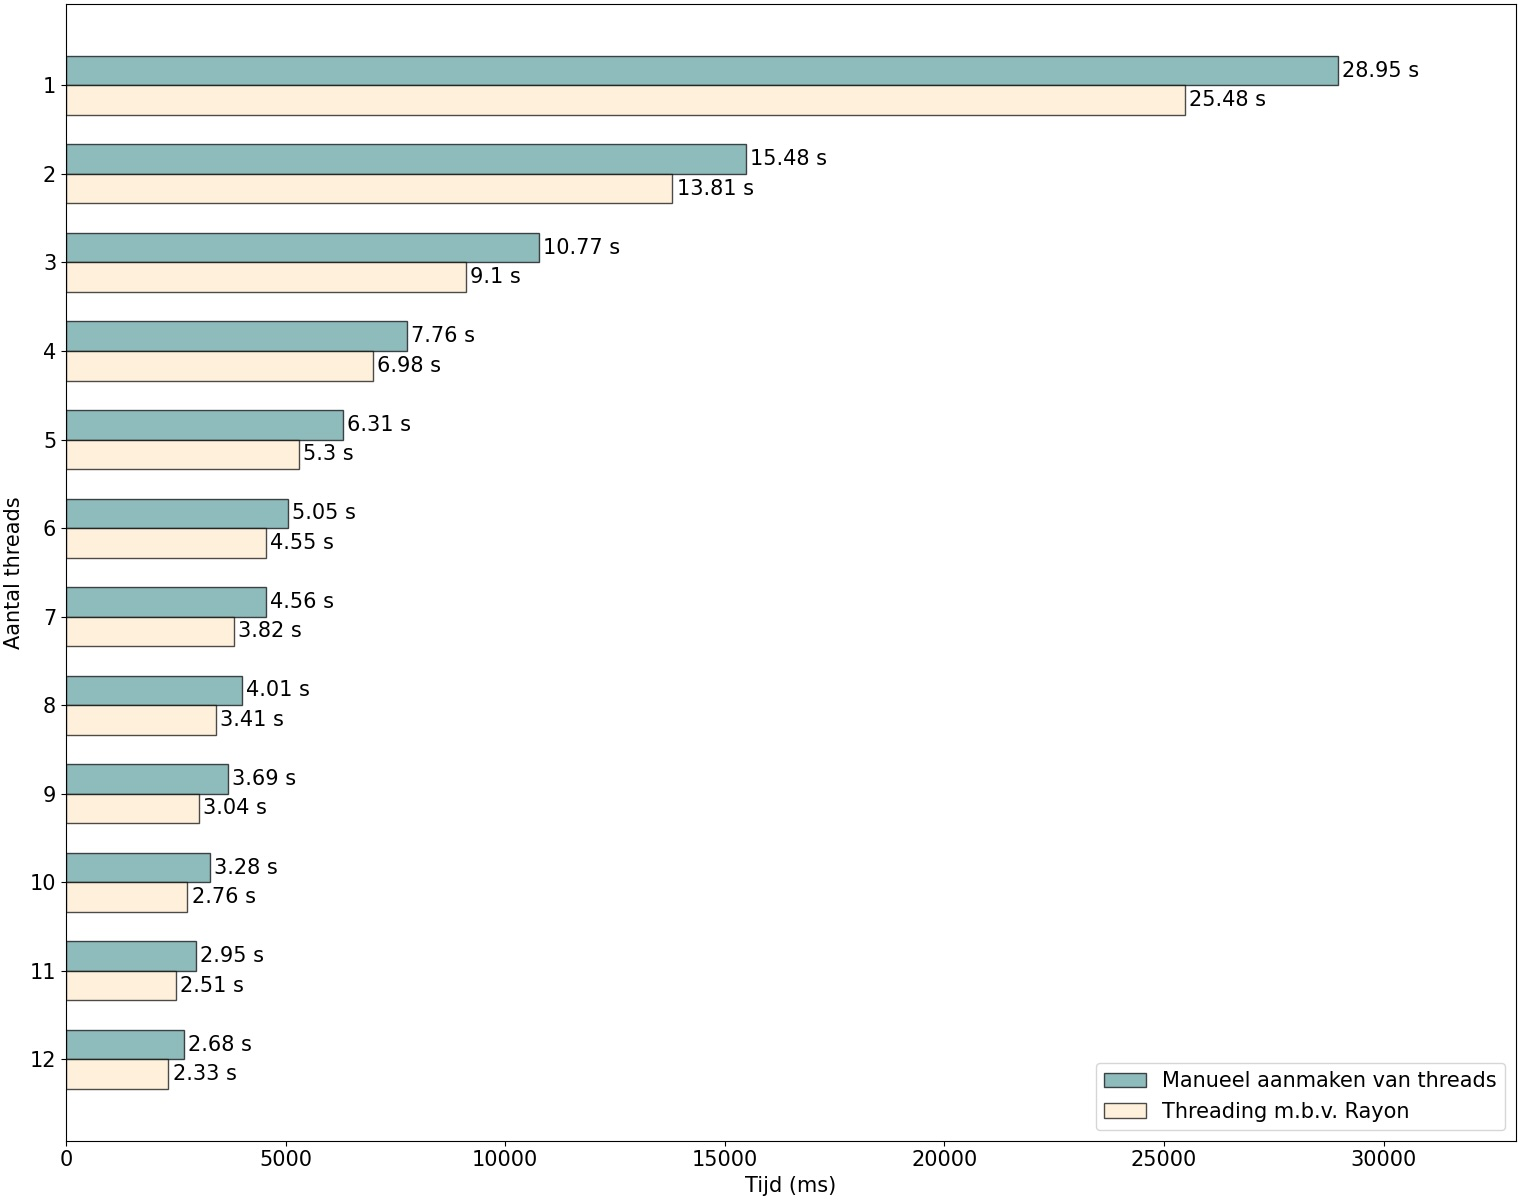
\includegraphics[width=0.7\linewidth]{threading_default_vs_rayon}}\\[4ex] % [4ex] om wat extra vertical spacing in te voegen

    \subfloat[Relatieve versnelling ten opzichte van uitvoering op 1 thread.]{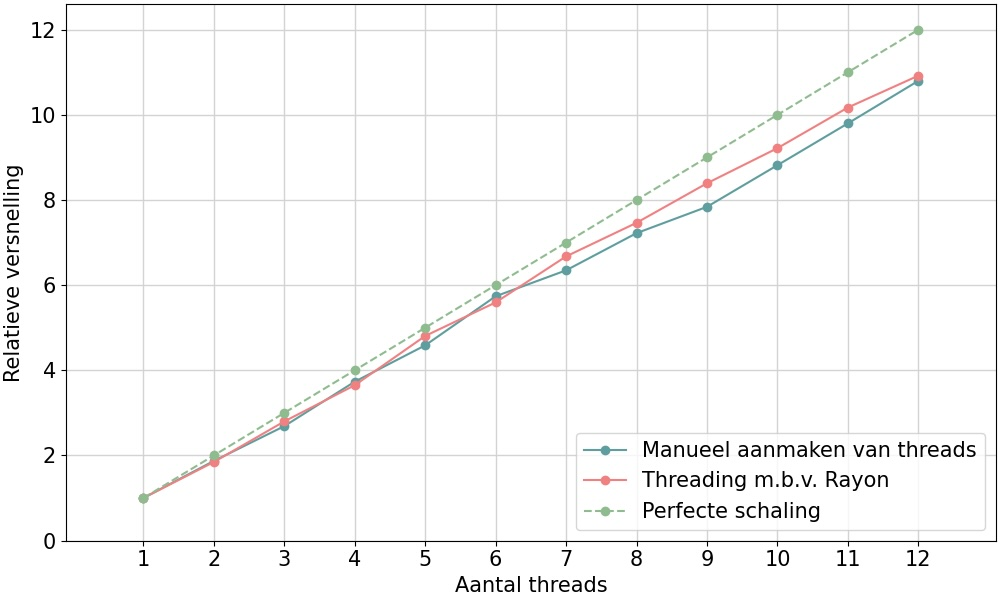
\includegraphics[width=0.7\linewidth]{threading_default_vs_rayon_relative}}
    \caption{Tijdsmeting om het Swiss-Prot peptidebestand zonder missed cleavages te zoeken in een index met sparseness factor 3 ter grootte van 5\% van UniProtKB.}\label{fig:threading_default_vs_rayon}
\end{figure}

Naast het verschil in performantie zijn er nog andere voordelen verbonden aan het gebruik van Rayon.
De code is namelijk veel simpeler en daarom ook beter te onderhouden.
Dit motiveert onze keuze om finaal gebruik te maken van Rayon.

\section{Performantie}\label{sec:performantie}
Nu we verschillende manier verkend hebben om suffix arrays op te bouwen is het interessant om onze implementatie te vergelijken met suffixbomen.
Op basis hiervan kunnen we daarna vaststellen welke verbeteringen we gemaakt hebben, als deze indexstructuur goed genoeg schaalt om toepasbaar te zijn op de volledige UniProtKB databank en in welke tijd de peptides gezocht kunnen worden.

\subsection{Opbouwen}
Figuur~\ref{fig:array_building} visualiseert de tijd nodig om de indexstructuur op te bouwen in combinatie met het geheugenverbruik.
Er is duidelijk een mooie tijdswinst verkregen, wat een bonus is voor het lokaal opbouwen van indexen.
Voor het opbouwen van de index op UniProt is dit echter minder van belang aangezien dit proces slechts een vier tal keren per jaar moet gebeuren.
Zolang de nodige CPU tijd hiervoor niet langer is dan enkele dagen is dit acceptabel.
Een veel belangrijkere vaststelling is het maximale geheugenverbruik tijdens opbouwen.
Ook deze is drastisch gedaald.
Dit is exact de reden dat we deze indexstuctuur gekozen hebben.
Wanneer we het resultaat voor Swiss-Prot extrapoleren naar UniProtKB gebruikmakende van de assumptie dat UniProtKB $\pm$ 500x groter is dan is de verwachting dat er ongeveer 1.2 TB RAM nodig is.
Dit is nog steeds een grote hoeveelheid, maar dit wordt al praktisch mogelijk op een server gericht op het uitvoeren van geheugenintensieve taken.

\begin{figure}[H]
    \centering
    \subfloat[Tijd nodig om de index op te bouwen.]{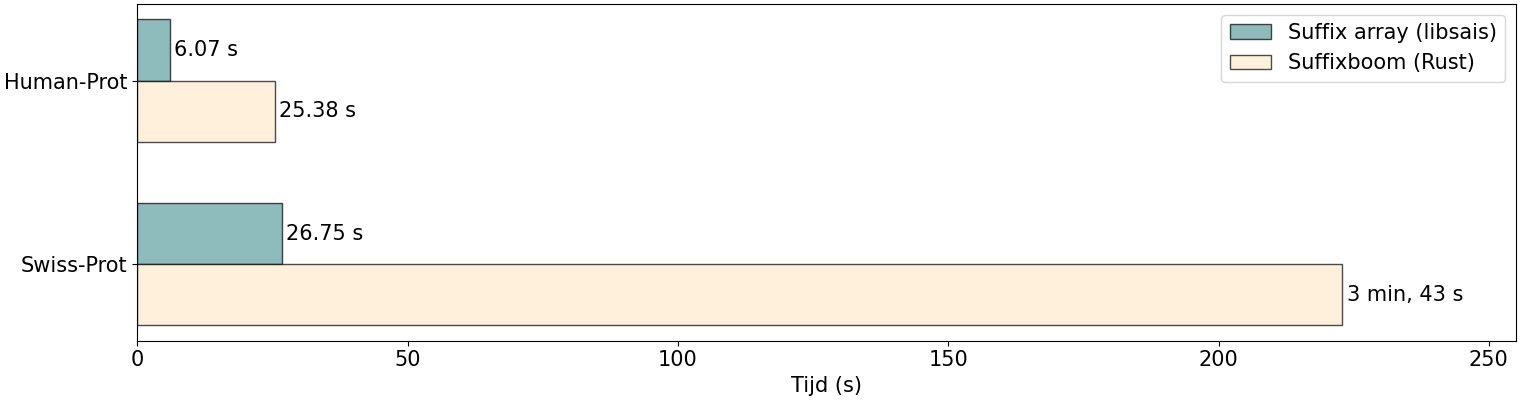
\includegraphics[width=\linewidth]{building_array_libsais_time}}\\[4ex] % [4ex] om wat extra vertical spacing in te voegen

    \subfloat[Maximaal geheugengebruik tijdens het opbouwen van de suffixboom.]{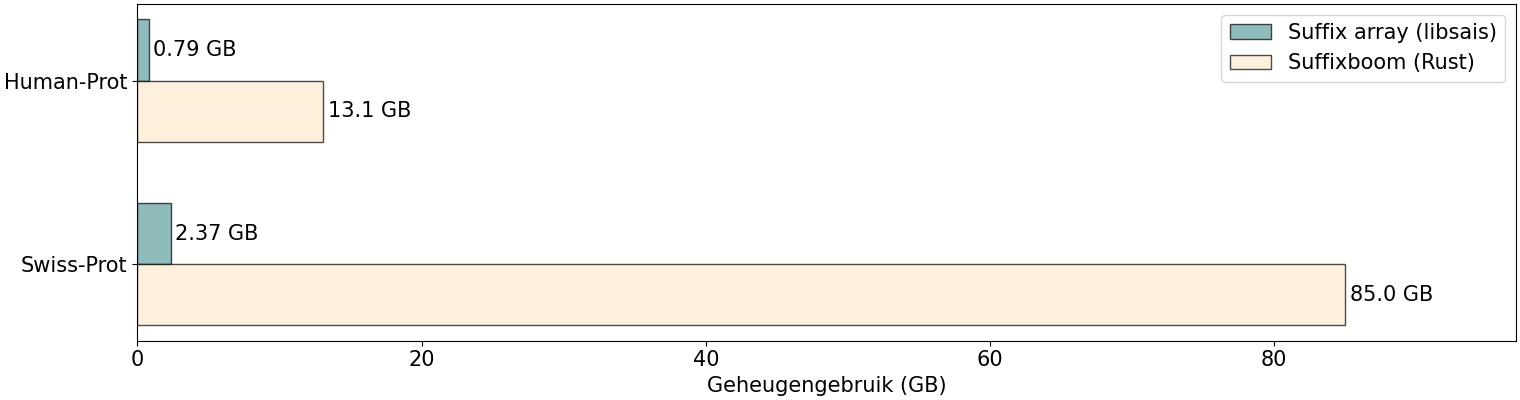
\includegraphics[width=\linewidth]{building_array_libsais_memory}}
    \caption{Vergelijking tussen de nodige tijd en hoeveelheid geheugen om een suffix array met LibSais op te bouwen of een suffixboom in onze eigen Rust implementatie. De tijd en het geheugengebruik zijn gemeten met het unix \texttt{time} commando. Als invoerbestand gebruiken we hier de Swiss-Prot of Human-Prot eiwitdatabank.}\label{fig:array_building}
\end{figure}

\subsection{Zoeken}
Aangezien er geen voorberekening gebeurt van LCA's is het enkel nuttig om de zoektijd inclusief het berekenen van de LCA te bekijken.
De tijd tot een match levert ons nog niet alle nodige informatie op (zoals dit het geval was bij de suffixboom).

\subsection{Beperken van het maximaal aantal matches}\label{subsec:maximaal-aantal-matches}
Op het eerste zicht leek de performantie voor sommige bestanden dramatisch veel slechter.
Dit is zichtbaar voor het Human-Prot peptidebestand in~\ref{fig:cutoff_humanprot}~(a).
Na wat onderzoek bleek dat het berekenen van de LCA* erg traag werd indien er een groot aantal matches waren.
Daarom is er besloten om een cut-off in te stellen.
Indien een peptide meer dan dat aantal matches heeft wordt verondersteld dat de root de kleinste gemeenschappelijke voorouder is van alle matches.
Uit onderzoek~\cite{unipept_cutoff} blijkt dat dit in de praktijk in de overgrote meerderheid van de gevallen ook effectief het geval is.
Zo zijn er slechts $\pm$ 13000 peptides met meer dan 10000 eiwitten matchen.
Hierbij was voor 95\% van de peptides de LCA de root en slechts voor 200 peptides een resultaat op \textit{species} niveau.
\\
\begin{figure}[H]
    \centering
    \subfloat[Bereken de LCA* voor alle matches.]{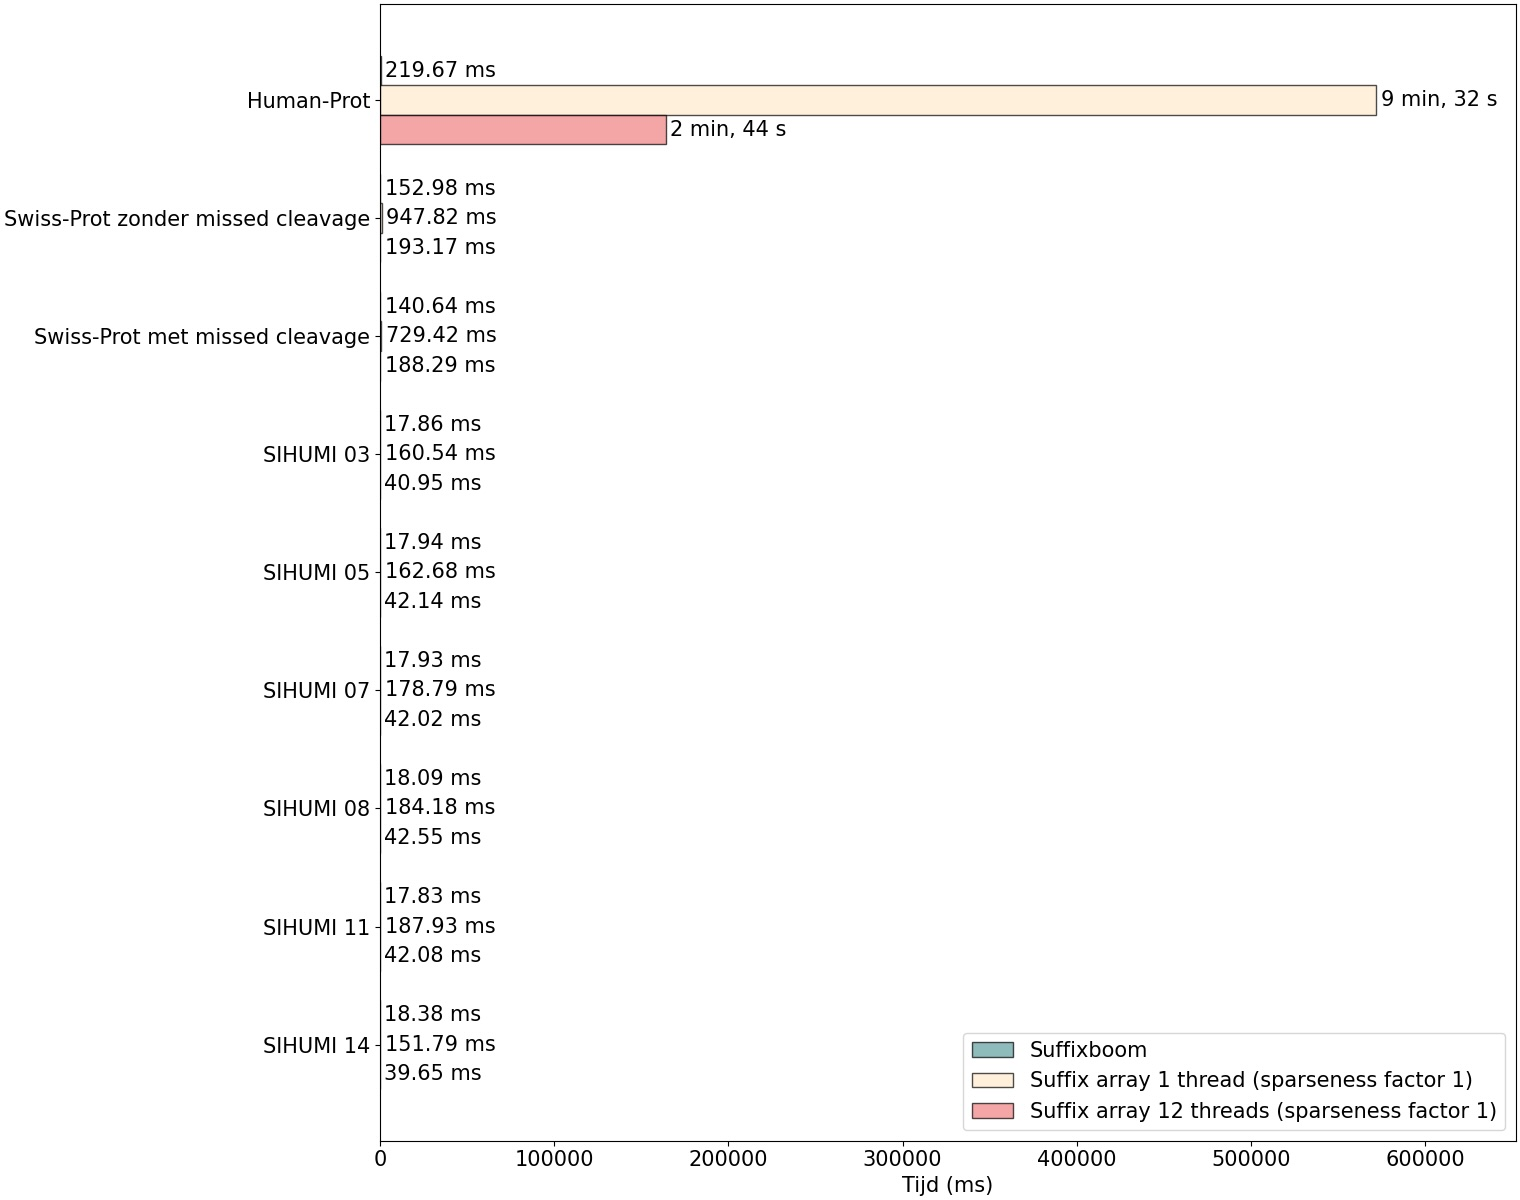
\includegraphics[width=0.7\linewidth]{no_cutoff_humanprot_search}}\\[4ex] % [4ex] om wat extra vertical spacing in te voegen

    \subfloat[Bereken de LCA* als er minder dan 10000 matches zijn.]{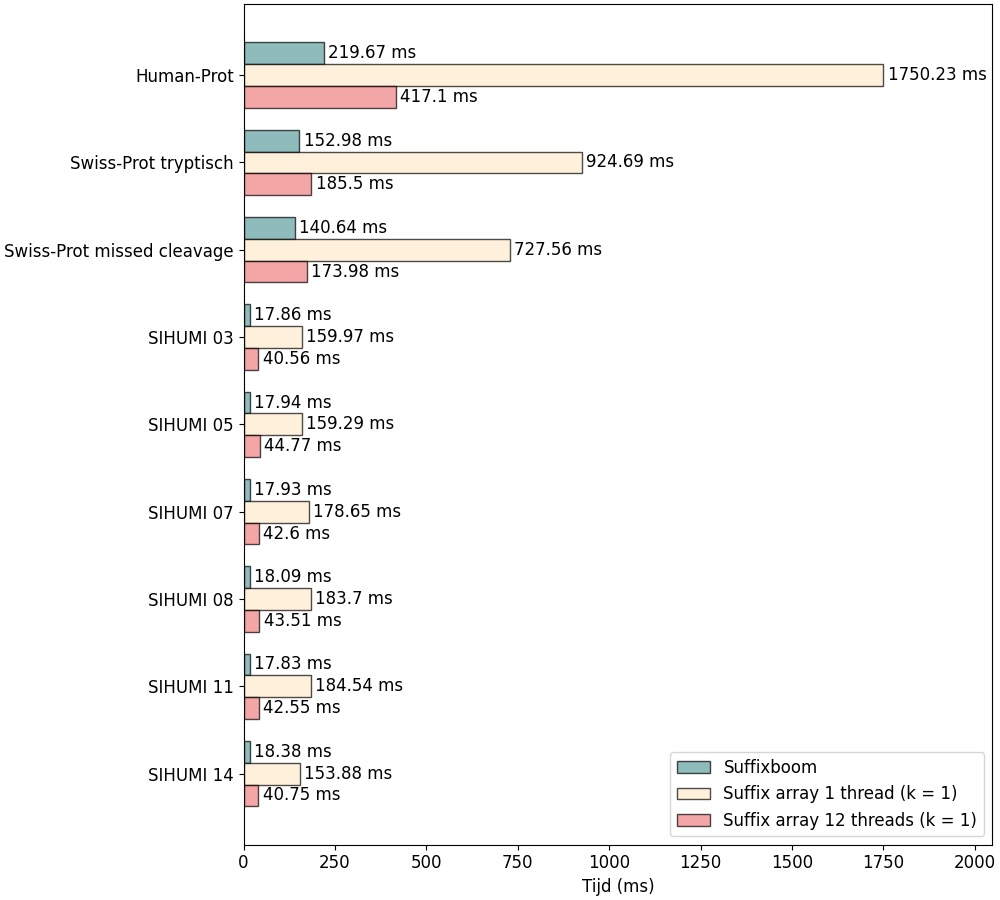
\includegraphics[width=0.7\linewidth]{cutoff_humanprot_search}}
    \caption{Berekenen van de LCA* (inclusief zoeken) voor alle peptiden in Human-Prot zonder en met cut-off.}\label{fig:cutoff_humanprot}
\end{figure}

In Figuur~\ref{fig:cutoff_humanprot} is duidelijk te zien dat de uitvoeringstijd drastisch daalt wanneer de cut-off op 10000 matches geplaatst wordt.
Als we dit specifiek bekijken voor de Human-Prot peptidebestanden en eiwitdatabank is de uitvoeringstijd maar liefst een 300x sneller.
Bovendien is ook hier het informatieverlies minimaal.
Van de 250000 peptides zijn er 12 peptides die een ander resultaat verkrijgen in de output.
Deze 12 entries zijn echter slechts twee verschillende peptides (die gewoon meerdere malen voorkomen in het peptidebestand).
Dit zijn de peptides \texttt{EKP} en \texttt{SKE}.
Indien we de LCA* effectief berekenen is het resultaat in beide gevallen 9606, terwijl we met een cut-off de root (1) terug geven.
\\ \\
Nu we het zoeken in de suffix array afgesteld hebben aan de hand van een cut-off is het interessant om te kijken hoe de zoekperformantie zich verhoudt ten opzichte van het zoeken in een suffixboom.
Bij een 1 op 1 vergelijking is het zoeken in de suffixboom duidelijk sneller.
Dit is ook exact wat we verwacht hadden.
In de praktijk is het zoeken in een suffix array 5 tot 10 maal trager voor onze testbestanden.
Een deel van deze extra zoektijd kan opgevangen worden door gebruik te maken van parallel zoeken.
Indien we hier gebruik van maken duurt het zoeken van 100000 peptides opnieuw enkele tientallen tot honderden milliseconden voor 100000.
Natuurlijk zouden we ook het zoeken in een suffixboom kunnen parallelliseren.
Daarbij zal de absolute tijdswinst echter veel kleiner zijn doordat dit al zo snel is.

\section{UniProtKB}
Zoals eerder vermeld levert een ruwe extrapolatie op dat we $\pm$ 1.2 TB aan geheugen nodig zou hebben om een index voor UniProtKB op te bouwen.
Hierbij werd er echter van uitgegaan dat UniProtKB 500x meer eiwitten dan Swiss-Prot bevat.
Dit is een overschatting van de realiteit waar UniProt op dit moment \textit{slechts} $\pm$ 440 keer groter is.
Dit zorgt ervoor dat het opbouwen mogelijks al haalbaar is op HPC van UGent waar nodes beschikbaar zijn die ongeveer 940 GB aan beschikbaar geheugen hebben.
Na dit te proberen bleek dit ook effectief al haalbaar.
Figuur~\ref{fig:build_uniprot} toont de nodige tijd en hoeveelheid geheugen om dit te realiseren.
Opvallend hierbij is dat het Libsais algoritme hier trager is dan libdivsufsort, terwijl dit voor alle kleinere datasets net omgekeerd was.
Afhankelijk van je dataset is het ene algoritme dus sneller dan het andere.
Het geheugengebruik van beide algoritmes blijft echter erg gelijkaardig, wat het belangrijkste is voor ons.
\\
\begin{figure}[H]
    \centering
    \subfloat[Tijd nodig om een index voor UniProtKB te bouwen.]{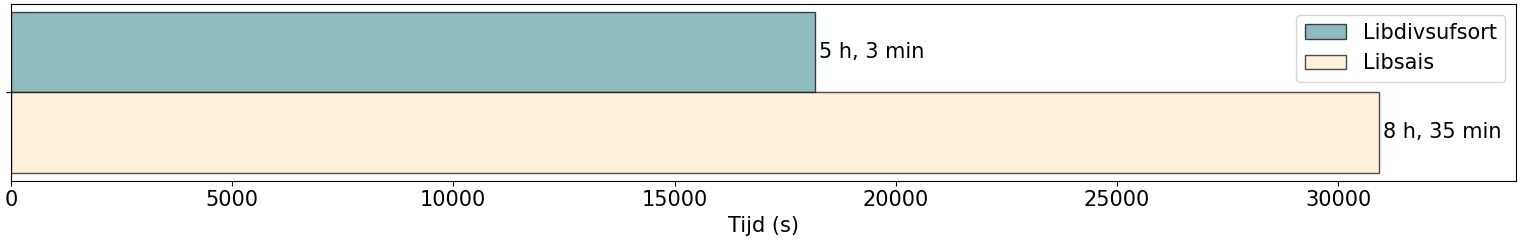
\includegraphics[width=\linewidth]{build_uniprot_time}}\\[4ex] % [4ex] om wat extra vertical spacing in te voegen

    \subfloat[Maximale hoeveelheid geheugen gebruikt tijdens het opbuowen van een index voor UniProtKB.]{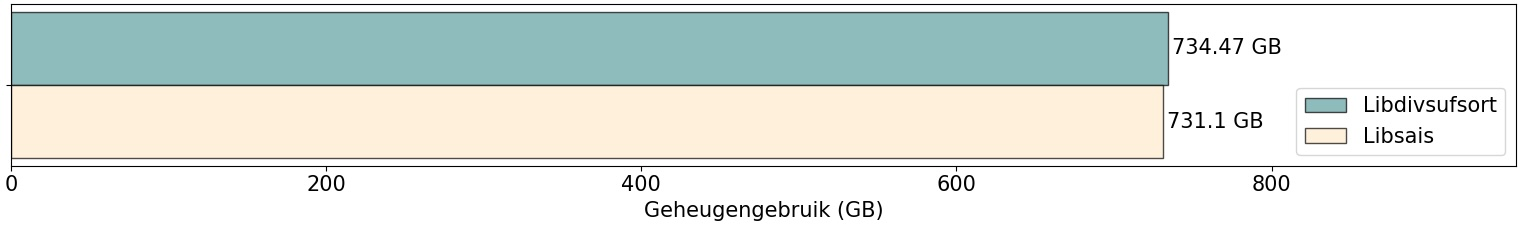
\includegraphics[width=\linewidth]{build_uniprot_memory}}
    \caption{Statistieken voor het opbouwen van een SA voor UniProtKB}\label{fig:build_uniprot}
\end{figure}

Een volgende stap na het opbouwen van de volledige SA was het beslissen van de sparseness factor.
Zoals eerder aangegeven in de conclusie van sectie~\ref{subsec:zoeken-in-sparse-suffix-arrays} willen we deze sparseness factor zo laag mogelijk kiezen, met als restrictie dat de SSA nog steeds in het geheugen moet kunnen gehouden worden.
De beschikbare machines die UniPept hosten hebben elk $pm$ 0.5 TB RAM ter beschikking.
Dit wil zeggen dat we de resulterende index hierin moeten krijgen, en ook nog genoeg overhead moeten laten zodat de machine zeker niet out-of-memory gaat tijdens het hosten van de index en het verwerken van meerdere requests.
Praktisch gezien komt dit er op neer dat we gebruik maken van sparseness factor 3. % TODO: of 2, moeten we eens testen
Dit resulteert in een SA van 231.81 GB.
In combinatie met de tekst (86.93 GB) resulteert dit in een totale indexgrootte van 318,74 GB, wat comfortabel in de 0.5 TB past.
Indien we sparseness factor 2 zouden gebruiken is dit niet meer het geval. % TODO: zou er wel in kunnen, ongeveer 440 GB in het totaal nodig, maar is dit nog "oké?"
Dan komt de totale indexgrootte op $\pm$ 450 GB uit, wat te dicht ligt bij de grens.

    
    \chapter{Andere indices}\label{ch:andere-indices}
Naast suffixbomen en suffix arrays bestaan er ook nog enkele andere interessante indexstructuren.
We behandelen in dit hoofdstuk FM- en R-indices.
Deze maken achterliggend gebruik van suffix arrays, maar zorgen ervoor dat de index zelf kleiner wordt doordat niet de volledige tekst bijgehouden moet worden.


\section{FM-index}
Deze indexstructuur is vernoemd naar Ferragina en Manzini die dit als eerste beschreven hebben~\cite{fm_index}.
Een FM-index bestaat uit 3 essentiële componenten.
De Borrows-wheeler transformatie~\cite{bwt}, een (sparse/compressed) suffix array en bitvectoren die de rank-operatie ondersteunen.
Het opbouwen van de index kan gebeuren in $O(n)$ met $n$ de lengte van de invoertekst.
Het zoeken van een match kan in $O(m)$ (met $m$ de lengte van de zoekstring).
Het zoeken inclusief het vinden van waar alle matches in de originele string zitten kan in $O(m + \text{|occ}(P, T)\text{|} \log n)$.
Hierbij is $\text{occ}(P, S)$ de set van alle string dat prefix $P$ matcht in de input tekst $T$.
Door gebruik te maken van de BWT heeft deze indexstructuur als voordeel dat niet de volledige tekst expliciet bijgehouden moet worden, waar dus een significante winst kan gemaakt worden ten opzichte van het gebruik van enkel een suffix array.
Aan de hand van een variant van de FM-index, de bidirectionele FM-index kan men bovendien gebruikmaken van een techniek om efficiënt inexacte matching, waarbij maximaal $x$ mismatches toegelaten zijn, uit te voeren.
Dit worden zoekschema's genoemd.

\subsection{Verschillende implementaties}
Om een goed beeld te krijgen over het geheugenverbruik tijdens het opbouwen hebben we verschillende bestaande FM-index implementaties getest.
Opnieuw focussen we ons vooral op het geheugenverbruik aangezien dit de primaire restrictie tijdens het opbouwen.
Tabel~\ref{tab:fm_index_building} geef een overzicht van de geteste implementaties.
Omdat ons einddoel is om UniProtKB te indexeren kunnen we ons opnieuw enkel focussen op de 64 bit implementaties, aangezien de UniProtKB te groot is voor 32 bit implementaties.
Als referentie kunnen we vergelijking met de resultaten uit Tabel~\ref{tab:sa_building} waaruit we konden concluderen dat het opbouwen van een suffix array voor de Swiss-Prot eiwitdatabank kan in 1.86 GB RAM\@ (bij het gebruik van 64 bit integeres).
Wanneer we dit vergelijken met de resultaten voor de geteste FM-index implementaties, zien we dat deze bijna twee maal zo veel geheugen nodig hebben.
Omwille hiervan hebben we deze optie niet verder verkend.

\begin{table}[H]
    \begin{minipage}{\linewidth}
        \centering
        \resizebox{\textwidth}{!}{
            \begin{tabular}{l l S[table-format=-2.2] S[table-format=-2.2] S[table-format=-1.2] S[table-format=-1.2]}
                Algoritme & Programmeertaal & \multicolumn{2}{c}{Tijd (in s)} & \multicolumn{2}{c}{Geheugen (in GB)} \\
                \hline\hline
                &                         & {32 bit} & {64 bit} & {32 bit} & {64 bit} \\
                \cline{3-6}
                \url{https://crates.io/crates/fm-index}     & Rust                    & {-}      & 33.92    & {-}      & 3.22     \\
                \url{https://github.com/simongog/sdsl-lite} & C++                     & {-}      & 27.74    & {-}      & 3.70     \\
                \url{https://github.com/ocfnash/FM-Index}   & Cython met C++ bindings & 57.94    & {-}      & 1.96     & {-}      \\
                \hline
            \end{tabular}
        }
        \caption{Uitvoeringstijd en maximaal geheugengebruik voor het opbouwen van een FM-index aan de hand van verschillende algoritmen voor de Swiss-Prot eiwitdatabank.
        Afhankelijk van als de implementatie 32 bit of 64 bit integers gebruikt is een andere kolom ingevuld. Een - staat voor niet getest. Deze testen werden lokaal uitgevoerd op een M1 Pro MacBook Pro. De specificaties hiervan zijn terug te vinden in tabel~\ref{tab:macbook_hardware}.}
        \label{tab:fm_index_building}
    \end{minipage}
\end{table}


\section{R-index}
R-indices~\cite{r_index1, r_index2} zijn een verdere evolutie van de FM-index waarbij run-length encoding (RLE) toegepast wordt op de BWT\@.
De index heeft grootte $O(r)$ met $r$ het aantal BWT runs van de input tekst van lengte $n$.
De winst op vlak qua geheugengebruik wordt groter naarmate er meer herhaling voorkomt in de tekst die geïndexeerd wordt.
Om het na te gaan wat het effect hiervan is op de onze eiwitdatabanken hebben we de R-index getest op de eerste 0.5\%, 1\%,\ldots van de volledige UniProtKB databank.
Figuur~\ref{fig:sa_vs_r_index} visualiseert het geheugenverbruik in de resulterende indexgrootte.
Merk op dat het geheugenverbruik tijdens het opbouwen en de grootte van de resulterende R-index meer dan verdubbelt bij het overgaan van 2\% (1651521046 tekens) naar 4\% (3319904170) van UniProtKB\@.
Dit komt doordat er bij de databank van 2\% of minder, minder tekens zijn dan de maximale 32 bit integer waarde.
Hierdoor maakt de R-index tot hier gebruik van 32 bit integers.
Bij de databanken die bestaan uit 4\% van UniProtKB, wordt deze 32 bit integer limiet overschreden.
Hierdoor schakelt de R-index over naar het gebruik van 64 bit integers.
\\ \\
Op vlak van geheugenverbruik zien we duidelijk dat het opbouwen van een suffix array minder geheugen vraagt, maar dat het verschil tussen de resulterende suffix array en R-index procentueel groter en groter wordt.
Dit is de winst die verkregen wordt door het gebruik van de run-length encoding.
Natuurlijk zouden we bij de suffix array ook vrij simpel de resulterende index kunnen verkleinen door de SA sparse te maken.
Hierbij zal op een gegeven punt de winst in indexgrootte teniet gaan door de tekst die altijd volledig opgeslagen wordt.
Bij het gebruik van sparseness factor $k = 3$ voor de grootste geteste index zou de totale index voor de suffix array terug gedrongen worden tot 15.31 GB\@.
Van deze 15.31 GB is 4.17 GB de tekst zelf.
\\ \\
Vanwege het sterk verhoogde geheugenverbruik tijdens het opbouwen hebben we ervoor gekozen om deze optie niet verder te verkennen in deze masterproef.
Bovendien kunnen zoals geïllustreerd de indexgrootte voor de suffix array al enkele factoren kleiner maken door deze sparse te maken.

\begin{figure}
    \centering
    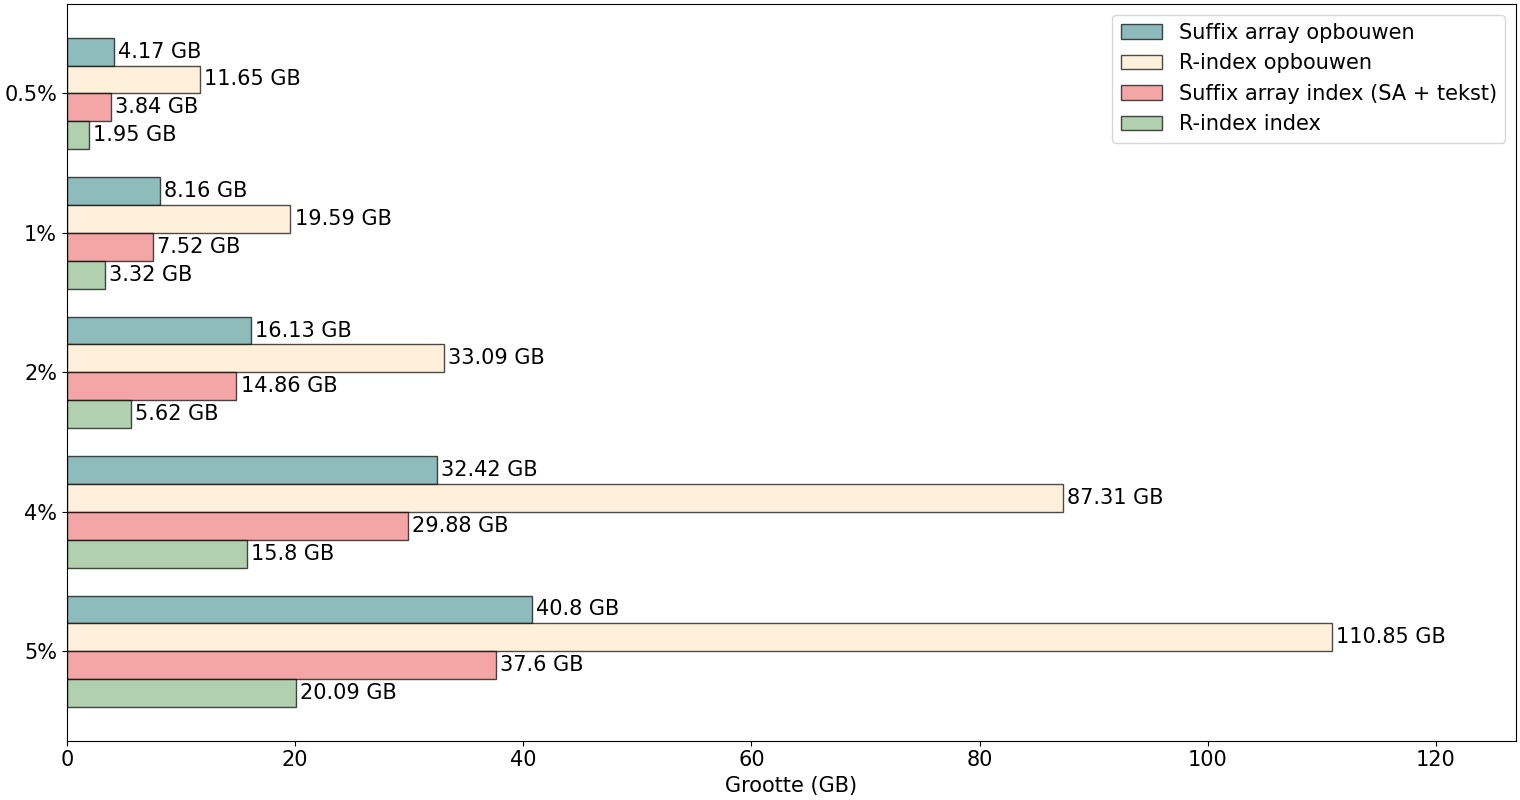
\includegraphics[width=0.8\linewidth]{sa_vs_r_index}
    \caption{Het geheugengebruik tijdens het opbouwen van de suffix array, of R-index en de grootte van de resulterende index. De index wordt opgebouwd voor verschillende subsets van UniProtKB. In elke test gaat het om de eerst $x$ procent van de database. Bij suffix arrays sparseness factor $k = 1$ gebruikt. Indien een andere factor gebruikt zou worden, heeft dit enkel invloed op de grootte van de resulterende index.}
    \label{fig:sa_vs_r_index}
\end{figure}


    
    \chapter{Een nieuwe UniProtKB-index voor Unipept}\label{ch:een-nieuwe-uniprotkb-index-voor-unipept}
In de vorige hoofdstukken hebben we suffixbomen, suffix arrays, FM-indices en R-indices verkend als indexstructuren die toegepast kunnen worden om een proteïnedatabank te indexeren.
Hieruit bleek dat een suffix array de laagste geheugenvereisten heeft tijdens het opbouwen.
In dit hoofdstuk gaan we dieper in op het opbouwen van een index voor UniProtKB gebruikmakende van een suffix array, en het in productie brengen ervan.
Aangezien we de huidige Unipept index willen vervangen door deze nieuwe indexstructuur behandelen we bovendien ook nog enkele extra gewenste features.

\section{Opbouwen van de SA}\label{sec:opbouwen-van-de-sa}
Zoals vermeld in sectie~\ref{subsec:opbouwen} levert een ruwe extrapolatie op dat we 1.2 TB RAM nodig hebben om een suffix array op te bouwen voor UniProtKB\@.
Hierbij wordt er echter van uitgegaan dat UniProtKB 500 keer meer proteïnen dan Swiss-Prot bevat.
Dit is een overschatting van de realiteit waar UniProtKB op dit moment \textit{slechts} $\pm$ 440 keer groter is.
Dit zorgt ervoor dat het opbouwen mogelijks al \textbf{haalbaar is op de HPC van UGent} waar nodes beschikbaar zijn tot 940 GB RAM\@.
Na dit te proberen bleek \textit{slechts} 740 GB RAM nodig.
Dit is minder dan verwacht omdat onder andere de NCBI taxonomy in het geheugen gehouden wordt.
Deze blijft even groot, onafhankelijk van de grootte van de proteïnendatabank.
Figuur~\ref{fig:build_uniprot} toont de nodige tijd en hoeveelheid geheugen om dit te realiseren.
\textbf{Opvallend hierbij is dat de libsais implementatie hier trager is dan libdivsufsort}, terwijl dit voor alle kleinere datasets net omgekeerd was.
Afhankelijk van de dataset is het ene algoritme dus sneller dan het andere.
Het geheugengebruik van beide algoritmen blijft echter erg gelijkaardig, wat het belangrijkste is voor ons.
\\
\begin{figure}[H]
    \centering
    \subfloat[Tijd nodig om een SA-index voor UniProtKB te bouwen.]{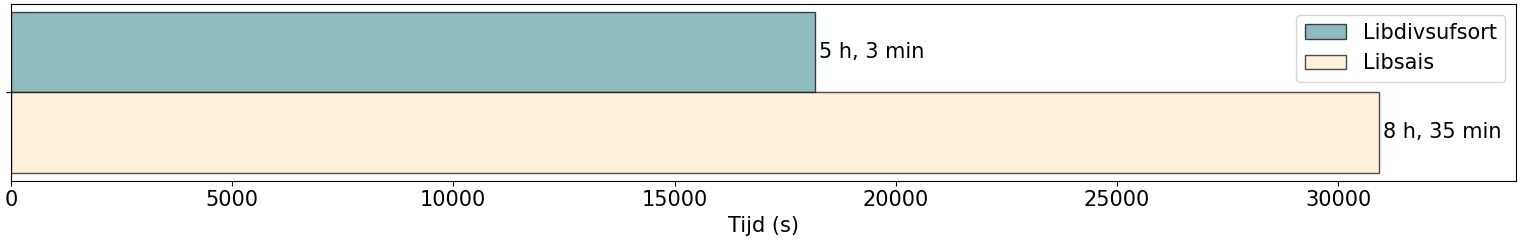
\includegraphics[width=\linewidth]{build_uniprot_time}}\\[4ex] % [4ex] om wat extra vertical spacing in te voegen

    \subfloat[Maximale hoeveelheid geheugen gebruikt tijdens het opbouwen van een SA-index voor UniProtKB.]{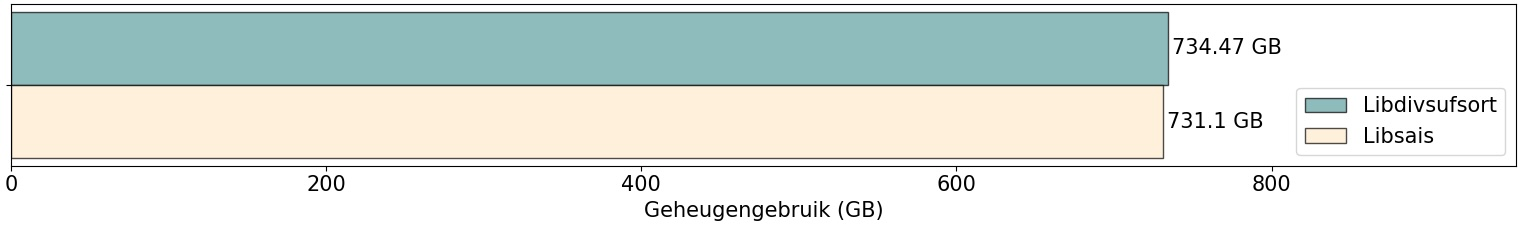
\includegraphics[width=\linewidth]{build_uniprot_memory}}
    \caption{Statistieken voor het opbouwen van een SA voor UniProtKB.}\label{fig:build_uniprot}
\end{figure}

\section{Een sparseness factor kiezen}
Een volgende stap na het opbouwen van de volledige SA bestaat uit het kiezen van de optimale sparseness factor.
Zoals eerder aangegeven in de conclusie van sectie~\ref{subsec:zoeken-in-sparse-suffix-arrays} willen we deze sparseness factor zo laag mogelijk houden, met als restrictie dat de sparse suffix array (SSA) nog steeds in het werkgeheugen moet passen.
Uit Figuur~\ref{fig:search_sparseness} (a) bleek namelijk dat het kiezen van een hogere sparseness factor een dramatische impact op de zoektijd van korte peptiden heeft.
Dit effect zal nog versterkt worden bij het gebruik van een grotere databank.
\\ \\
De beschikbare machines die Unipept hosten hebben elk $\pm$ 0.5 TB RAM ter beschikking.
Dit wil zeggen dat we de resulterende index hierin moeten krijgen, en ook nog genoeg ruimte moeten overlaten zodat de machine zeker niet crasht tijdens het hosten van de index en het verwerken van meerdere requests tegelijk.
Figuur~\ref{fig:uniprot_index_size_sparsenessfactors} toont een overzicht van de indexgrootte voor verschillende sparseness factors.
Aangezien we ongeveer 0.5 TB RAM ter beschikking hebben, zal \textbf{sparseness factor k = 3} de kleinste factor zijn die comfortabel in het geheugen past.
We hebben hiervoor namelijk al 322 GB RAM nodig.
Hierbij moet natuurlijk nog wat overhead gerekend worden voor de mapping van suffix naar proteïne, en alle annotaties die bij een proteïne horen bij te houden.
Bovendien bevatten deze servers ook nog andere databanken om verdere aggregaties te berekenen.
Indien we sparseness factor 2 zouden gebruiken komt de totale indexgrootte uit op $\pm$ 440 GB\@.
Dit op zich zou nog net in de machine passen, maar laat niet genoeg ruimte voor de andere processen.

\begin{figure}[h!]
    \centering
    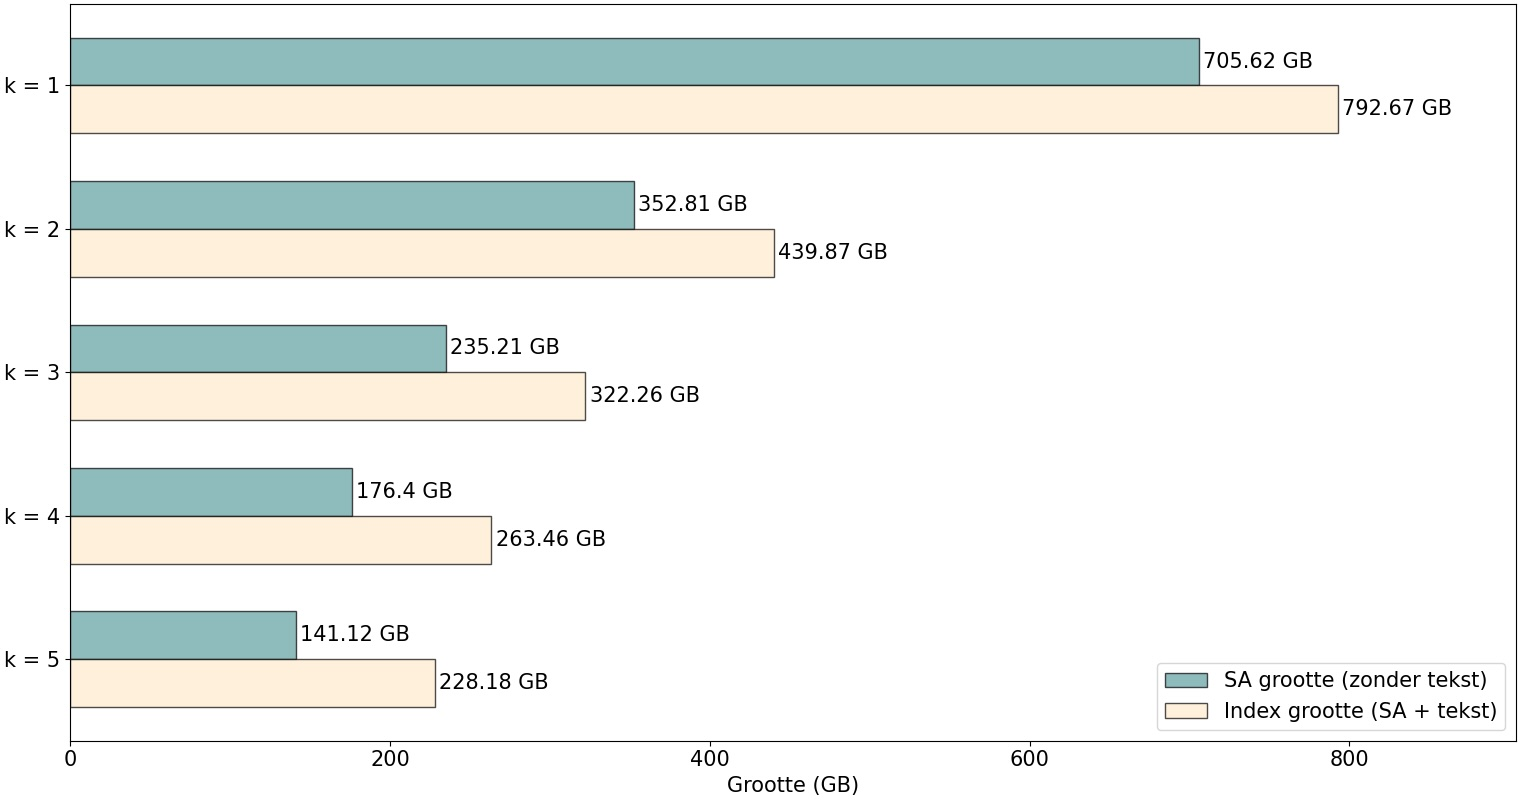
\includegraphics[width=0.8\linewidth]{uniprot_index_sizes}
    \caption{Grootte van de SA en totale index opgebouwd op UniProtKB voor sparseness factor $k = 1, 2, 3, 4, 5$.}
    \label{fig:uniprot_index_size_sparsenessfactors}
\end{figure}

\section{Isoleucine en leucine gelijkstellen}\label{sec:isoleucine-en-leucine-equivalentie}
Naast het vinden van exacte matches is het vinden van inexacte matches ook interessant.
Vooral het vinden van matches waarbij we de aminozuren I (isoleucine) en L (leucine) aan elkaar gelijkstellen is een belangrijke optie in de huidige Unipept index.
\textbf{Deze twee aminozuren kunnen niet gedifferentieerd worden door een massaspectrometer omdat ze een identieke massa hebben}.
Door deze restrictie is het voor onderzoekers erg nuttig om alle matches te vinden waar een I ook een L kan zijn, of omgekeerd.
Om deze vorm van inexacte matching toe te voegen aan de index gebruikmakende van een suffix array zijn er meerdere opties:
\begin{enumerate}
    \item \textbf{Twee indices:} Bouw een extra index waarbij in de tekst elke L ook door een I vervangen wordt, of vice versa.
    Bij het verwerken van een zoekopdracht wordt deze afgehandeld door de juiste index afhankelijk van de gekozen configuratie.
    Indien I en L gelijkgesteld worden hoeft er slechts één bijkomende operatie uitgevoerd te worden.
    Dit is dezelfde vervangoperatie die uitgevoerd is op de originele tekst bij het opstellen van de index.
    Deze optie wordt niet verder uitgewerkt omdat we willen vermijden dat we twee volledig aparte indices moeten hosten, waardoor het geheugengebruik zou verdubbelen.
    \item \textbf{Index waarbij I $\neq$ L:} Genereer de varianten van de gezochte peptide \textit{on the fly} tijdens het zoekproces.
    Hierbij kan gebruikgemaakt worden van het feit dat twee peptiden die identiek zijn, behalve dat elke locatie waar een I een L kan staan (of vice versa), een gelijkaardig zoekpad afleggen in de SA\@.
    Deze zoekpaden splitsen enkel wanneer het teken dat verwerkt wordt (uit de proteïnedatabank) tijdens de binary search een I, J, K of L is.
    Dit zorgt ervoor dat voor een willekeurig patroon een groot stuk van de zoekboom gemeenschappelijk zal zijn.
    Ook al zal dit ervoor zorgen dat we tijdens het zoekproces meestal snel kunnen snoeien, we zullen steeds $2^{q}$ opties moeten verkennen.
    Hierbij is $q$ de som van het aantal I's en L'en is in de peptide.
    \item \textbf{Index waarbij I = L:} Bouw de index voor een variant van de UniProtKB database.
    Hierbij vervangen we elke I door een L, of vice versa, en bouwen we dus een index op waarbij I gelijkgesteld is aan L\@.
    Tijdens het zoeken van een peptide doen we dezelfde vervanging, waarna we alle matches hebben waarbij I gelijkgesteld is aan L\@.
    Indien we I niet gelijk willen stellen aan L, kunnen we achteraf de foute matches wegfilteren aan de hand van de originele proteïnedatabank.
\end{enumerate}

In de volgende secties worden de tweede en derde aanpak verder uitgewerkt.

\subsection{Index waarbij I $\neq$ L}\label{subsec:index-waarbij-i-neq-l}
Wanneer de indexstructuur zelf gebouwd is met I niet gelijkgesteld aan L, moeten we alle verschillende IL-combinaties tijdens het zoekproces verkennen.
Hierbij is het echter belangrijk om te weten dat er ook bepaalde extreem slechte gevallen bestaan waarbij de zoekruimte erg groot wordt, en we niet efficiënt kunnen snoeien.
De sequenties waarop we zoeken zijn namelijk niet random verdeeld over alle karakters van het alfabet.
Biologisch gezien komen bepaalde aminozuursequenties veel vaker voor.
Eén van deze patronen zijn de zogenaamde \textit{leucine rich repeats}~\cite{leucine_rich_repeats}.
Dit zijn sequenties waarin een reeks L'en na elkaar voorkomt.
In UniProtKB bestaat er een \textbf{sequentie waar maar liefst 2397 L'en na elkaar voorkomen}.
Dit is de proteïne met \textit{accession number} \texttt{A0A1Q9EZQ0}.
Wanneer we nu ook weten dat in UniProtKB ook reeksen aan I's voorkomen zorgt dit voor bepaalde extreem slechte gevallen.
Zo is hier \textbf{ook een proteïne met 641 opeenvolgende I's} (accession number: \texttt{A0A5J4P3H7}).
In het slechtste geval zou een gebruiker dus een sequentie van 641 I's of L'en kunnen proberen te matchen.
Dit zorgt ervoor dat we in de zoekboom $2^{641} \approx 9.12 \cdot 10^{192}$ opties moeten proberen.
Het grootste deel van deze opties zal niet voorkomen, waardoor de takken van deze boom allemaal extreem kort zullen zijn.
Dit zal echter verwaarloosbaar zijn ten opzichte van het gigantisch aantal opties.
Om dit in perspectief te plaatsen: Men schat dat er in het totaal $10^{79}$ atomen in het universum zijn~\cite{atoms_in_universe} en dat het universum ongeveer $4.36^{20} \approx 6.16 \cdot 10^{12}$ milliseconden oud is~\cite{age_universe}.
Zelfs als het controleren van één optie minder dan een milliseconde duurt, dan zou dit dus nog onmogelijk zijn.
\textbf{Om de zoektijd en het geheugengebruik te beperken, hebben we ervoor gekozen om twee vormen van restricties op te leggen wanneer I en L gelijkgesteld worden}.
\begin{enumerate}
    \item Laat maximaal 5 seconden aan zoektijd per peptide toe.
    \item Laat per peptide in totaal maximaal 34 I's en L'en toe.
\end{enumerate}
Deze twee restricties samen moeten de servers deels helpen beschermen tegen Denial of Service attacks.
In de praktijk wordt normaal de tijdslimiet van 5 seconden eerst bereikt.
Dit vertaalt zich naar een sequentie van ongeveer 25 I's of L'en.
Elke keer we één extra teken zouden willen toelaten verdubbelt de zoektijd.
Zo duurt het al één minuut om een sequentie met 30 opeenvolgende I's of L'en te zoeken.
Wanneer we echter nog veel meer I's of L'en toelaten stuiten we vrij snel op een geheugenlimiet.
Om te voorkomen dat het programma meer geheugen probeert te vragen dan dat de server heeft, waarna het crasht, hebben we beslist maximaal 34 I's of L'en toe te laten.
In het slechtste geval gebruikt één enkele thread hierbij iets meer dan 2 GB RAM\@.
Aangezien het zoeken multithreaded is, moeten we dus zeker 20 GB aan vrij geheugen voorzien wanneer de index ingeladen is.
\textbf{Wanneer we deze limieten testen door alle testpeptidebestanden te zoeken in de volledige UniProtKB databank worden deze limieten geen enkele keer bereikt}.
\\ \\
In de praktijk vertaalt het gelijkstellen van I en L op deze manier zich naar een \textbf{vrij kleine overhead}.
Deze beperkte overhead valt te zien in Figuur~\ref{fig:uniprot_search}.
Deze figuur toont ook onmiddellijk de zoekperformantie waarbij I $\neq$ L op UniProtKB\@.
Zoals verwacht op basis van de resultaten voor de kleinere Swiss-Prot en Human-Prot proteïnedatabanken, is dit zoeken inderdaad extreem snel.
% TODO: schrijf hier iets bij in vergelijking met de huidige unipept index qua snelheid

\begin{figure}[ht]
    \centering
    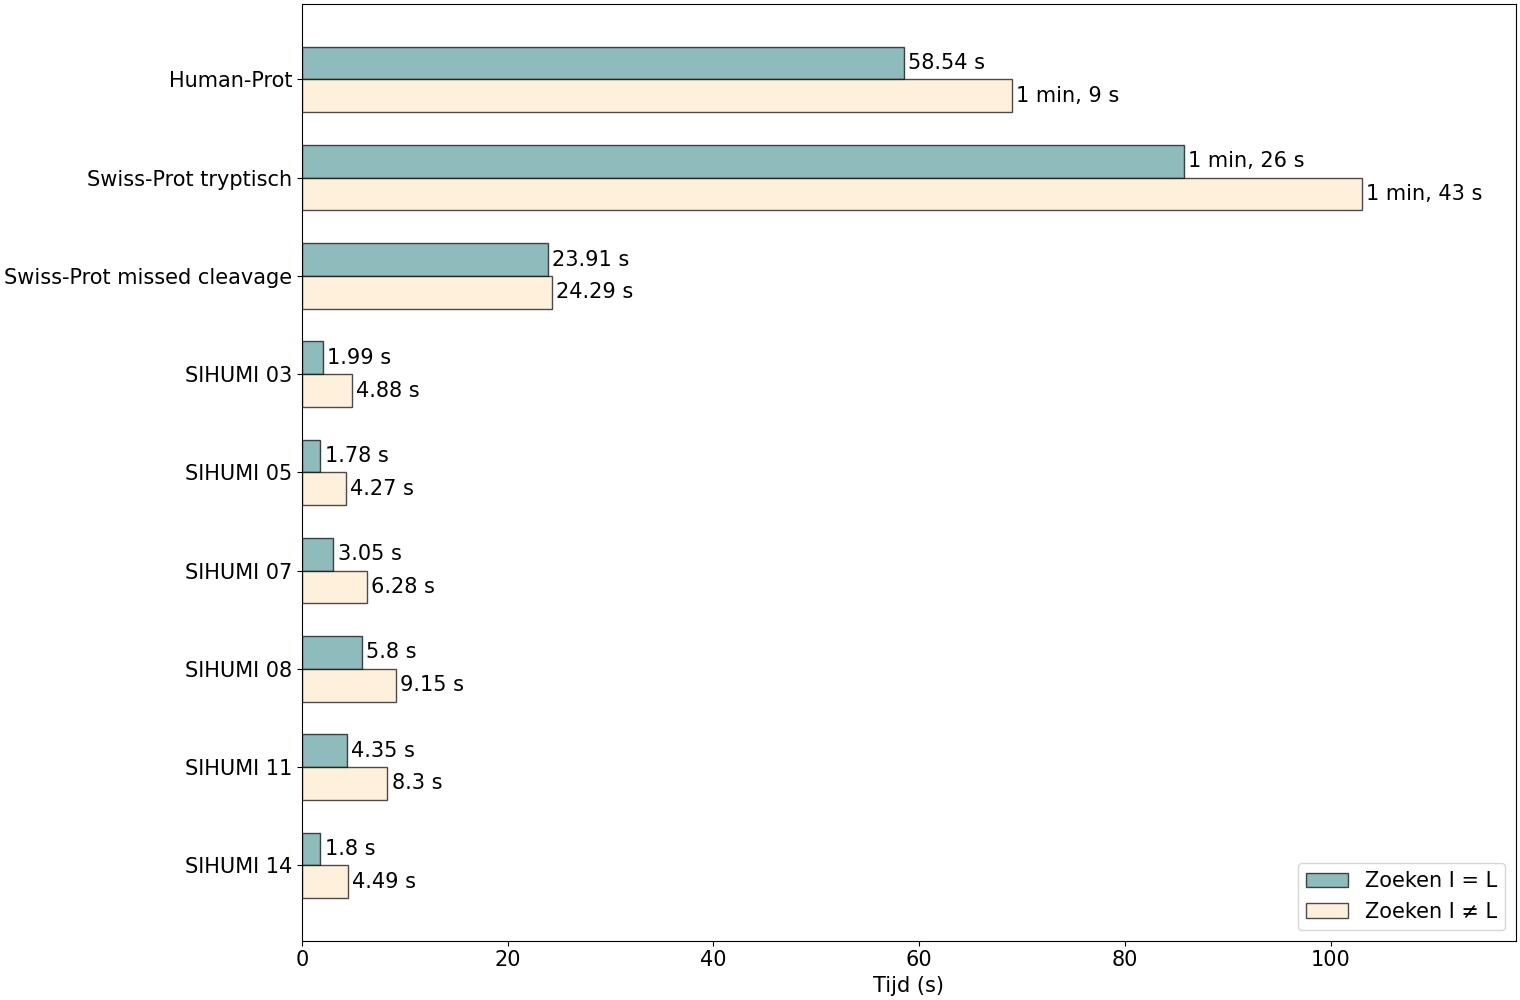
\includegraphics[width=0.95\linewidth]{uniprot_searchtime_standard_vs_il_equality}
    \caption{Zoektijd in UniProtKB (Swiss-Prot + TrEMBL) met en zonder het gelijkstellen van I en L met een SA met sparseness factor $k = 3$. De index zelf is opgebouwd op basis van een tekst waar I $\neq$ L.}
    \label{fig:uniprot_search}
\end{figure}

\subsection{Index waarbij I = L}
Een andere optie om zoeken waarbij I en L gelijkgesteld zijn mogelijk te maken is door de index specifiek voor dit geval op te bouwen.
Hierbij wordt in de originele tekst elke L vervangen door een I, of vice versa, om op deze aangepaste tekst een index te bouwen.
Wanneer we in de gezochte peptiden hetzelfde doen, vinden we alle matches, waarbij een I en L gelijkgesteld zijn.
Dit is duidelijk erg simpel, en bovendien efficiënt.
\\ \\
Door het zoekproces licht aan te passen, kunnen we bovendien nog steeds de matches vinden waarbij I $\neq$ L\@.
Dit kan via volgend stappenplan:
\begin{enumerate}
    \item \textbf{Zoek alle matches} in de SA, waarbij I = L\@.
    Hiervoor moeten we in elke peptide dezelfde vervangoperatie uitvoeren als tijdens het bouwen van de suffix array.
    \item \textbf{Filter de ongeldige matches weg}.
    Dit kunnen we doen door voor alle matches te controleren op elke positie waar een I of L is, als daar hetzelfde teken staat als in de tekst.
    Wanneer in de peptide een L staat, en de tekst een I (of omgekeerd), wil dit zeggen dat deze match ongeldig is, want ze is enkel gevonden vanwege het gelijkstellen van I aan L tijdens het zoeken.
    Merk op dat we hiervoor de originele tekst nodig hebben, en niet de aangepaste tekst die gebruikt is bij het bouwen van de suffix array.
    Gelukkig moeten we niet allebei deze teksten in het geheugen houden, via enkele kleine aanpassingen tijdens het zoeken kan de originele tekst perfect gebruikt worden om te zoeken in de suffix array van de gemodificeerde tekst.
\end{enumerate}

Dit stappenplan is niet alleen \textbf{simpel}, maar het bevat ook \textbf{geen extreem slechte gevallen} zoals bij de index waarbij we I $\neq$ L stellen, en dan alle opties proberen verkennen.
Bovendien is ook de impact van de filterstap beperkt aangezien enkel locaties waar een I of L staat in de peptide gecontroleerd moeten worden.
Andere tekens moeten we nooit controleren, aangezien het zoeken in de SA ons al garandeert dat deze overeenkomen.
Er is dus geen nood aan een combinatie van systemen die de server moeten beschermen tegen de slechtste gevallen, die extreem lang konden duren, en bovendien ook veel geheugen vereisen.
\\ \\
Naast deze voordelen blijkt ook dat deze manier van zoeken iets sneller is in het algemeen.
Dit valt te zien in Figuur~\ref{fig:uniprot_search_il_equal}.
Een laatste voordeel is dat het gelijkstellen van I en L de standaard optie is in de huidige Unipept UI\@.
Dit is net ook wat hier het minste werk vereist tijdens het zoeken.
Vanwege al deze voordelen kiezen we ervoor om van deze zoekstrategie gebruik te maken.

\begin{figure}[ht]
    \centering
    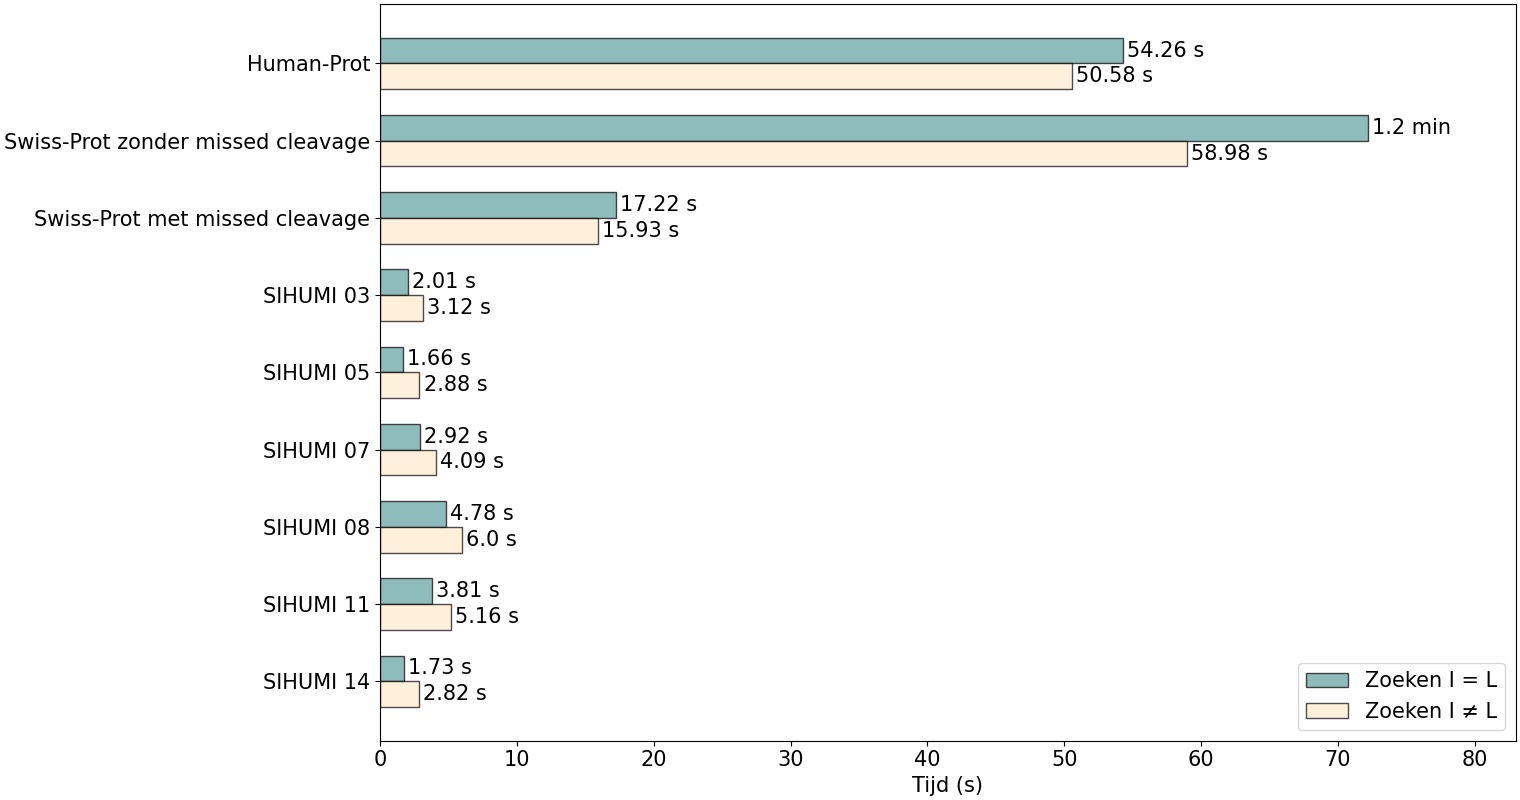
\includegraphics[width=0.95\linewidth]{uniprot_searchtime_standard_vs_il_equality_il_equal_index}
    \caption{Zoektijd in UniProtKB (Swiss-Prot + TrEMBL) met en zonder het gelijkstellen van I en L met een SA met sparseness factor $k = 3$. De index zelf is opgebouwd op basis van een tekst waar I = L.}
    \label{fig:uniprot_search_il_equal}
\end{figure}

Eén iets merkwaardig is dat voor onze kleinere SIHUMI testbestanden het zoeken met I $\neq$ L sneller is, ook al is dit net minder werk.
Dit komt omdat zonder dit filteren er meer resultaten zijn.
Deze extra resultaten moeten allemaal meegenomen worden in het berekenen van de LCA*, maar ook tijdens het serializeren van de resultaten naar een JSON-bestand.
Bovendien zorgt een grotere hoeveelheid data ook voor een tragere doorstroming van de index naar de Unipept API\@.
Bij de grotere testbestanden wordt er in verhouding meer tijd aan het zoeken gespendeerd, waardoor daar de verwachte tijdwinst wel zichtbaar is.

\section{Taxonomische analyse}\label{sec:taxonomische-analyse}
Door het gebruik van suffix arrays moet de taxonomische analyse volledig uitgevoerd worden tijdens het zoekproces zelf.
Dit heeft zowel voor- als nadelen.
\\ \\
Het grootste nadeel is de \textbf{extra overhead per zoekopdracht}.
In de oude index was het enkel nodig alle matches te zoeken, waarna de voorberekende LCA onmiddellijk opgehaald kon worden.
Nu moeten we deze LCA ook nog berekenen.
Indien we dit zouden willen oplossen is er nood aan een manier om de boomstructuur te reconstrueren op een geheugenefficiënte manier.
Hiervoor zijn de extra tabellen van Enhanced Suffix Arrays nodig.
\\ \\
Anderzijds zijn er ook enkele voordelen verbonden met het berekenen tijdens het zoekproces zelf.
Zo hebben we \textbf{minder geheugen} nodig, wat erg belangrijk is aangezien het geheugengebruik al erg hoog is tijdens het opbouwen van de suffix array.
Bovendien laat dit ook toe dat we vrij kunnen kiezen welke aggregatiemethode we gebruiken.
De oude Unipept index maakte gebruik van een (minder interessante) variant van \textbf{LCA*}.
Dit werd gedaan om het voorberekenen efficiënter te maken.
Bij suffixbomen hebben we zelf gebruik moeten maken van de standaard LCA methode om dit op te lossen.
Bij suffix arrays kunnen we vrij gebruik maken van LCA*, en blijft de performantie bovendien erg goed.
Een laatste, belangrijk, voordeel is dat er \textbf{geen extra werk nodig is om de taxon IDs van alle matches op te halen}.
In de huidige Unipept index is hier een significante hoeveelheid extra werk voor nodig, wat resulteert in een bottleneck bij de Peptonizer2000 tool~\cite{pep_gm}.


\section{Functionele analyse}\label{sec:functionele-analyse}
Een laatste feature die de nieuwe index moet ondersteunen is de functionele analyse uit Unipept.
Deze analyse wordt uitgevoerd door de verschillende GO, EC en INTERPRO termen die horen bij de gevonden matches te tellen.
Elk van deze termen is een korte string van 5 à 10 karakters lang, en kan vrij eenvoudig mee ingelezen worden en per proteïne bijgehouden worden.
Al deze annotaties samen, maken het databankbestand dat ingelezen wordt om de index mee op te bouwen ongeveer 24 GB groter.
Wanneer we deze informatie allemaal ingeladen hadden, bleek het programma echter ongeveer 105 GB extra RAM te gebruiken.
De verklaring hiervoor is dat Rust 24 bytes overhead heeft per vector, en 24 bytes overhead per string.
Om deze annotaties bij te houden, hadden we net één vector per proteïne nodig, en die vector bevatte een reeks aan korte strings (de annotaties zelf).
Om dit op te lossen heeft Tibo Vande Moortele een simpele compressiebibliotheek\footnote{\url{https://github.com/unipept/unipept-index/tree/main/fa-compression}} ontwikkeld voor deze annotaties.
Hierbij worden 2 karakters uit een annotatie gecomprimeerd naar 1 byte, en kunnen bovendien enkele tekens weggelaten worden.
Na het gebruik van deze bibliotheek resulteert dit in \textbf{10.5 GB extra geheugengebruik}, wat in de context van de al 320 GB grote index (wanneer de tekst ook meegerekend wordt) bijna verwaarloosbaar is.
Aangezien ook deze analyse \textit{on the fly} uitgevoerd wordt, heeft ook dit een negatieve impact op de performantie.
De volgende sectie gaat dieper in op de performantie van de finale indexstructuur.

\section{Vergelijking met andere tools}\label{subsec:vergelijking-met-andere-tools}
Naast Unipept zijn er nog andere tools die UniProtKB doorzoeken.
In deze sectie vergelijken we de performantie en eigenschappen van Unipept met de \textbf{Uniprot Peptide search tool}, de \textbf{Expasy ScanProsite tool}.
We zullen de versie van Unipept die de nieuwe index gebruikt Unipept 6.x noemen, aangezien de nieuwe index gebruikt zal worden vanaf Unipept 6.0, terwijl de oude versie Unipept 5.x genoemd wordt.
Vanwege de beperkte performantie van een aantal van deze tools zullen we ons beperken tot het opzoeken van één willekeurige peptide \texttt{ISPAVLFVIVILAVLFFISGLLHLLVR}.
Als referentie gebruiken we de zoektijd Unipept 6.x waarbij, zoals eerder vermeld, sparseness factor $k = 3$ gebruikt wordt.
Hierbij duurt het zoeken van de peptide \textbf{$\pm$ 3 milliseconden} en levert deze 50 matches op.
Wanneer we I en L gelijkstellen duurt dit opnieuw ongeveer 3 milliseconden, maar levert dit wel 52 matches op.
Hierbij wordt natuurlijk geen extra tijd geïntroduceerd door een API call over het internet aangezien deze index (nog) niet publiek beschikbaar is.

\subsection{UniProt peptide search tool}
De UniProt peptide search tool~\cite{uniprot_search_paper, uniprot_search_site} is een onderdeel van de UniProt site en laat toe om alle voorkomens van een bepaalde peptide te vinden in de volledige UniProtKB databank.
Als opties kunnen we kiezen om enkel in Swiss-Prot te zoeken, of in Swiss-Prot en TrEMBL\@.
Voor beide databanken kunnen we kiezen of we I en L aan elkaar willen gelijkstellen.
Deze features komen exact overeen met de eigenschappen van onze nieuwe indexstructuur, met de uitzondering dan Unipept extra analyses aanbiedt.
Qua performantie is deze tool echter extreem onstabiel.
Zo duurt het zoeken van \texttt{ISPAVLFVIVILAVLFFISGLLHLLVR} in de volledige UniProtKB databank \textbf{enkele seconden tot zelfs 20 minuten}.
Bovendien vermoeden we ook dat er een vorm van caching toegepast wordt aangezien het zoeken voor een tweede keer zo goed als onmiddellijk het resultaat geeft.
Dit maakt het benchmarken extreem moeilijk.
Zoals verwacht zijn de gevonden matches identiek aan de matches die onze nieuwe indexstructuur vindt.
Naast de variabele performantie faalt deze tool ook regelmatig tijdens het zoeken en ophalen van de resultaten.
\\ \\
Vanwege de extreem gelijkaardige mogelijkheden van deze tool hebben we contact opgenomen met UniProt om de vergelijking meer compleet te maken.
Hun eigen index werkt op basis van Apache Lucene\footnote{\url{https://lucene.apache.org/}}, waarbij alle proteïnen opgesplitst worden in 3-grammen.
Volgende sectie bevat de gestelde vragen, met de gegeven antwoorden.

\begin{description}[style=nextline]
    \item[How much memory is needed to build the index structure?]
    Answer: There is no specific requirement for the RAM.
    One of our users had tested that it works with 32 GB RAM\@.
    \item[How long does it take to build the index?]
    Answer: It depends on the hardware.
    We usually run it in a machine with 256 GB RAM to index the UniProtKB sequences plus the related information.
    It can take 1 to 2 days depending on how busy the machine is.
    \item[How much memory is needed to host the index?]
    Answer: We had been running the PeptideSearch services in a server with 256 GB RAM for many years and upgraded the RAM to 512 GB to improve the performance.
    \item[How many requests do you handle per day?]
    Answer: There are around 350 searches per day in April.
    \item[How many peptides does the average request contain?]
    Answer: Around 80\% of the cases search one peptide.
    \item[What percentage of requests treat isoleucine and leucine as equivalent? ]
    Answer: Around 6\% of the cases treat isoleucine=leucine.
    \item[What is the average time needed to handle 1 request? During our own testing we noticed that the performance can vary a lot from request to request. Is there an explanation for this?]
    Answer: If you are using the tool on our website, response times can vary due to several reasons:
    \begin{enumerate}
        \item Load of the server running PeptideSearch (currently running at PIR in Delaware, US)
        \item Load/availability of the dispatching server which is located at the EBI, UK)
    \end{enumerate}
\end{description}

Uit deze antwoorden kunnen we concluderen dat hun index lagere geheugenvereisten heeft.
Vermoedelijk komt dit door Apache Lucene geen hard-limit heeft om de index te kunnen gebruiken.
Het zal echter zoveel geheugen proberen gebruiken als het toegewezen krijgt, om zo onder andere caching toe te passen.
Dit verklaart waarschijnlijk ook deels de variabele performantie.
Afhankelijk van eerdere zoekopdrachten zijn verschillende stukken van de index waarschijnlijk sneller doorzoekbaar.
\\ \\
Interessant is ook dat 80\% van de zoekopdrachten uit één peptide bestaan, en dat slechts in 6\% van de gevallen I en L gelijkgesteld worden.
Dit is net het tegenovergestelde van de geregistreerde requests bij Unipept.
Vermoedelijk komt het verschil bij het gelijkstellen van I en L doordat dit standaard aan staat bij Unipept, terwijl dit bij UniProt net standaard uit staat.

\subsection{Expasy ScanProsite tool}
De Expasy ScanProsite tool~\cite{scanprosite} laat toe om aan de hand van motieven die lijken op reguliere expressies allerlei patronen te zoeken.
De beschrijving van motieven laat toe om onder andere wildcards, karakterklassen\footnote{Hiermee bedoelen we het toelaten van een reeks aan tekens op een bepaalde plaats. Dit is gelijkaardig aan de \texttt{[ABC]} syntax uit reguliere expressies, waar we een A, B of C toelaten.}, inverse klassen en herhalingen te specificeren.
De flexibiliteit van dit systeem is dus een sterk voordeel.
Een nadeel van deze tool is dat niet de volledige UniProtKB databank doorzocht wordt.
Er wordt enkel rekening gehouden met proteïnen die deel uit maken van een \textit{reference proteome}\footnote{Deze zogenaamde \textit{reference proteomes} zijn een collectie van proteïnen die door een bepaald organisme gemaakt kunnen worden, en die bovendien taxonomisch belangrijk bevonden worden. Deze laatste voorwaarde wil dus zeggen dat dit niet zomaar van elk organisme is, enkel van een selecte groep organismes die op basis van verschillende factoren belangrijk bevonden wordt. Een voorbeeld hiervan is de \textit{human reference proteome}. Dit zijn alle proteïnen die door een mens aangemaakt kunnen worden.}.
Dit komt erop neer dat ze bij UniProt 2024\_01 \textbf{slechts rekening houden met 85\thinspace152\thinspace388 van de 249\thinspace751\thinspace891 proteïnen}.
Wanneer we de zoekperformantie testen, duurt het zoeken van de ene peptide zo'n \textbf{5.5 minuten} zonder gelijkstellen van I en L en 10 minuten met het gelijkstellen van I en L\@.
Hierbij zijn er slechts 30 resp. 32 matches gevonden, wegens de deelverzameling van proteïnen die gebruikt wordt.

\subsection{Unipept 5.x}
Unipept 5.x kan, \textbf{op voorwaarde dat een peptide tryptisch is}, alle matches vinden in UniProtKB met de optie om I en L gelijk te stellen.
Onze willekeurig gekozen test peptide is tryptisch, dus vindt deze index zoals verwacht alle matches.
Bovendien gebeurt dit gebruikmakende van een API call in \textbf{$\pm$ 4 milliseconden}, wat duidelijk extreem veel sneller is dan de andere bestaande opties.
Opnieuw is de zoektijd hier al zo klein dat de invloed van het gelijkstellen van I en L niet te meten valt.
Het is echter een grote beperking dat dit enkel werkt voor tryptische peptiden, of peptiden met zogenaamde \textit{missed cleavages}.
Volgend voorbeeld illustreert dit.
Stel dat we nu de peptide \texttt{ILAKLFIS} zoeken.
Dit is geen tryptische peptide en bijgevolg kunnen er geen matches gevonden worden.
De nieuwe indexstructuur vindt echter 14 matches zonder I en L gelijk te stellen, en 207 matches bij het gelijkstellen van I en L\@.
\\ \\
Tot slot vergelijken we de zoektijd van Unipept 6.x en 5.x in meer detail aangezien één peptide hier geen goed zicht op geeft.
Hierbij berekenen beide indices ook de functionele en taxonomische analyses.
Het is belangrijk dat dit meegenomen worden tijdens het meten van de zoektijd, aangezien dit fundamentele functies van Unipept zijn.
We bekijken twee scenario's om zo een goed zicht op de performantie te krijgen.
In het eerste geval houden we rekening met \textit{missed cleavages}.
Dit is het meest realistische geval, aangezien stalen in de praktijk altijd \textit{missed cleavages} bevatten.
Figuur~\ref{fig:new_vs_old_unipept} geeft een overzicht voor de zoektijd op de SIHUMI peptidebestanden.
Hieruit blijkt dat Unipept 6.x 10 tot 100 keer sneller is dan Unipept 5.x.
Het andere geval is wanneer we een peptidebestand verwerken waarin enkel tryptische peptiden voorkomen.
Dit is niet realistisch, maar is het beste scenario voor Unipept 5.x aangezien de \textit{advanced missed cleavage handling} dan niet gebruikt moet worden.
Merk op dat Unipept 6.x wél \textit{missed cleavages} zal verwerken, aangezien dit geen negatieve invloed op de performantie heeft bij de nieuwe indexstructuur.
Figuur~\ref{fig:new_vs_old_unipept_tryptic} toont het verschil in zoektijd tussen Unipept 6.x en 5.x voor het tryptische Swiss-Prot peptidebestand.
Ter herinnering: dit bestand bestaat uit 100\thinspace000 tryptische peptiden.
Hieruit blijkt dat Unipept 6.x 33\% trager is dan Unipept 5.x wanneer I $\neq$ L, maar dat de zoektijd erg vergelijkbaar is wanneer I = L\@.
Dit verschil is acceptabel omdat we eigenlijk altijd rekening willen houden met \textit{missed cleavages}.
De enige reden dit amper gedaan werd in Unipept 5.x, is vanwege de grote impact op de performantie.
Bovendien kan Unipept 6.x ook ingezet worden voor niet-tryptische peptiden, wat niet mogelijk was voor Unipept 5.x en eerder.

\begin{figure}[h]
    \centering
    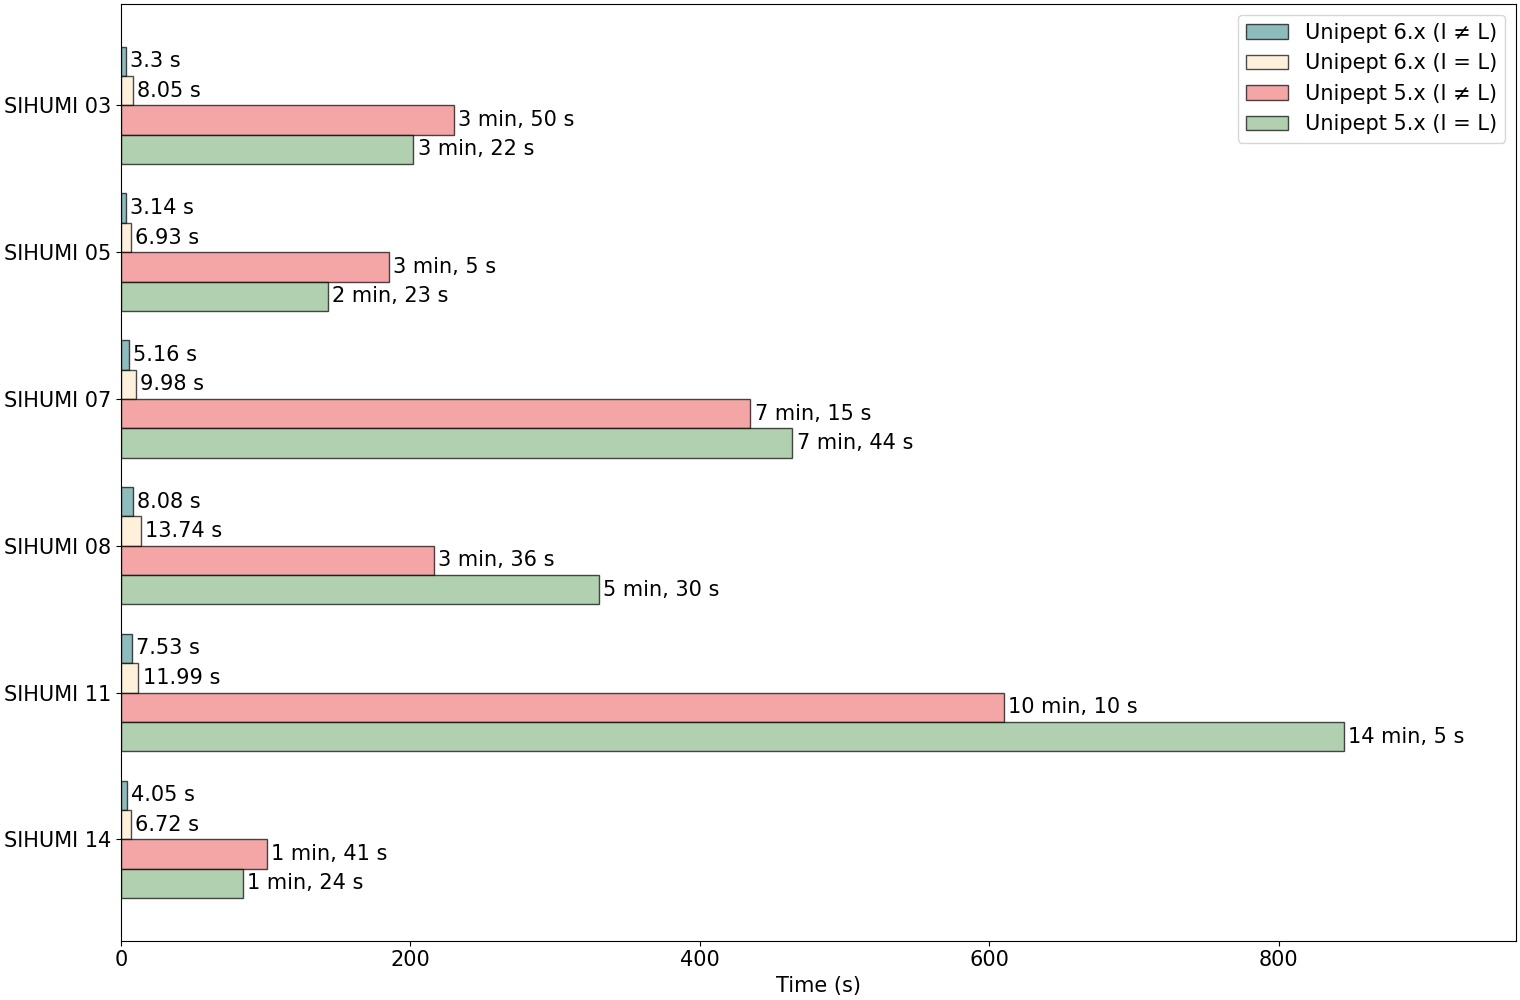
\includegraphics[width=0.85\linewidth]{new_vs_old_unipept}
    \caption{Unipept 6.x vs Unipept 5.x voor de SIHUMI peptidebestanden. Unipept 5.x is uitgevoerd met \textit{filter duplicate peptides} af, en \textit{advanced missed cleavage handling} aan. Op deze manier zullen beide versies alle peptiden zoeken, en ook \textit{missed cleavages} afhandelen. Merk op dat Unipept 6.x altijd \textit{missed cleavages} zal zoeken, en bovendien zelfs peptiden zal vinden die op een arbitraire manier gesplitst zijn.}
    \label{fig:new_vs_old_unipept}
\end{figure}

\begin{figure}[h]
    \centering
    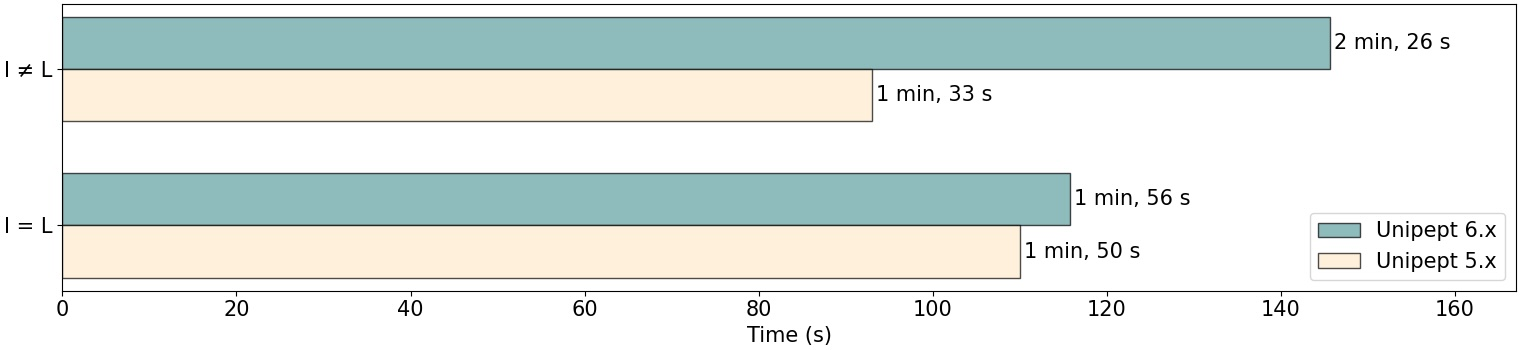
\includegraphics[width=0.85\linewidth]{new_vs_old_unipept_tryptic}
    \caption{Unipept 6.x vs Unipept 5.x voor het tryptische Swiss-Prot peptidebestand. Unipept 5.x is uitgevoerd met \textit{filter duplicate peptides} af, en \textit{advanced missed cleavage handling} af. Dit is het beste scenario voor Unipept 5.x, aangezien er geen \textit{missed cleavages} aanwezig zijn, en deze ook niet gezocht worden. Merk op dat Unipept 6.x wél \textit{missed cleavages} verwerkt, aangezien dit geen invloed heeft op de performantie bij de nieuwe indexstructuur.}
    \label{fig:new_vs_old_unipept_tryptic}
\end{figure}
\newpage
\section{Overzicht geheugenverbruik}
In de vorige secties zijn verschillende extra onderdelen besproken om de functionaliteiten van Unipept toe te voegen aan de nieuwe index.
Al deze extra onderdelen vragen extra geheugen, wat het totale geheugengebruik laat oplopen tot net geen 350 GB\@.
Figuur~\ref{fig:uniprot_memory_treemap} geeft een overzicht van het geheugenverbruik per onderdeel.
De volgende opsomming herhaalt kort voor elk onderdeel en welke rol deze speelt in het geheel.

\begin{itemize}
    \item Sparse suffix array: De sparse suffix array die opgebouwd werd op basis van de volledige UniProtKB databank.
    Op basis hiervan zoeken we efficiënt alle suffixen waarmee een peptide matcht.
    \item Tekst: Dit is de UniProtKB databank, waarbij alle proteïnen geconcateneerd worden tot één lange string.
    Tussen elke proteïne hangt hetzelfde, unieke scheidingsteken, en op het einde van de tekst een ander uniek teken.
    \item Functionele annotaties: De gecomprimeerde functionele annotaties die beschreven zijn in sectie~\ref{sec:functionele-analyse}.
    Op basis van deze annotaties wordt de functionele analyse van Unipept uitgevoerd.
    \item UniProt accession numbers: Elke proteïne in UniProtKB heeft een uniek ID (accession number).
    Voor elke proteïne die matcht met de gezochte peptide wordt dit ID als onderdeel van de output teruggegeven.
    \item Taxonomische annotaties: Het taxon ID dat per proteïne bijgehouden wordt.
    Op basis van deze taxon IDs wordt de LCA* van alle gevonden matches berekend.
    \item Suffix → proteïne: De sparse mapping die beschreven is in sectie~\ref{subsec:mapping-van-suffix-naar-proteine}.
    Deze mapping wordt gebruikt om de bijhorende proteïne te vinden van een gematchte suffix.
    \item NCBI taxonomy aggregator: Een object dat de gebruikte NCBI taxonomy om de LCA* aggregaties uit te voeren bevat.
    Aangezien deze opgebouwd wordt op basis van de NCBI taxonomy, is de grootte hiervan onafhankelijk van de gebruikte proteïnedatabank.
\end{itemize}

\begin{figure}[h]
    \centering
    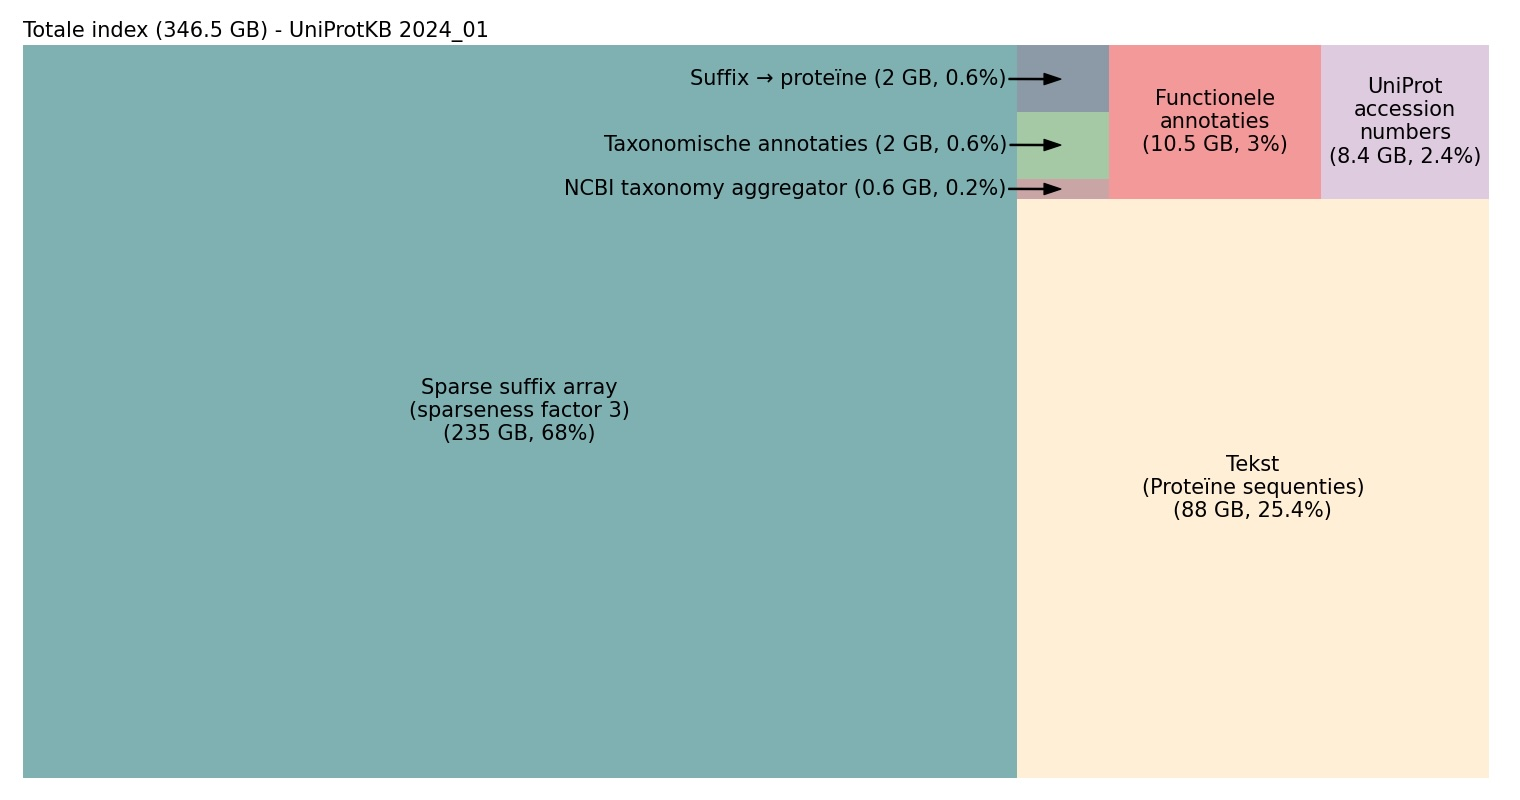
\includegraphics[width=0.76\linewidth]{uniprot_memory_treemap}
    \caption{Visualisatie van het totale geheugenverbruik voor de index gebouwd op basis van UniProtKB 2024\_01, gebruikmakende van sparseness factor $k = 3$ voor de SSA.
    In het totaal vraagt deze index 346.5 GB RAM, waarvan het grootste stuk gebruikt wordt door de SSA en de proteïne sequenties (de tekst) zelf.
    Naast de twee onderdelen die nodig zijn voor het matchen van de suffixen, is er nog een kleine 25 GB extra RAM nodig om de Unipept analyses aan te kunnen bieden, of om de ID's van de gevonden matches terug te kunnen geven.}
    \label{fig:uniprot_memory_treemap}
\end{figure}
\newpage
\section{Aanbieden van de nieuwe indexstructuur}\label{sec:aanbieden-van-de-nieuwe-indexstructuur}
In alle eerder vermelde benchmarks bespraken we enkel de zoektijd van een peptidebestand.
Bij het opstarten moeten we echter \textbf{eerst de indexstructuur inladen in RAM}.
Dit alleen duurt 20 tot 25 minuten.
We willen dit inladen slechts eenmalig doen om dan alle requests onmiddellijk te kunnen afhandelen.
Dit doen we aan de hand van een simpele \textbf{webserver} met de Axum crate~\cite{axum}.
Deze webserver laadt de indexstructuur in bij het opstarten, en blijft daarna wachten op HTTP-requests die een JSON-object bevatten met daarin de peptiden die we willen zoeken.
Op deze manier is dit probleem elegant opgelost, en kunnen we bovendien aan de hand van \textbf{JSON-bestanden} erg makkelijk de input verwerken, en de resultaten terugsturen.
Codefragment~\ref{fig:webserver_json_input} en~\ref{fig:webserver_json_output} geven een voorbeeld input en output.

\begin{listing}[H]
    \begin{minted}[frame=lines,framesep=2mm,linenos]{JSON}
{
  "peptides": [
    "LAKLFISAV",
    "ACCISDJLSDAAC"
  ],
  "equalize_I_and_L": true,
  "cutoff": 10000
}
    \end{minted}
    \caption{Voorbeeld JSON-input voor de webserver waarbij de peptiden \texttt{LAKLFISAV} en \texttt{ACCISDJLSDAAC} gezocht worden.
    Tijdens het zoeken worden I en L gelijkgesteld, en wordt de drempelwaarde B=10\thinspace000 gebruikt.
    Indien er meer matches zijn dan de drempelwaarde B, worden er slechts B matches terug gegeven en de resulterende LCA op 1 gezet.
    Dit laatste argument zou ook weggelaten kunnen worden aangezien de standaardwaarde gebruikt wordt.}
    \label{fig:webserver_json_input}
\end{listing}

\begin{listing}[h!]
    \begin{minted}[frame=lines,framesep=2mm,linenos]{JSON}
{
  "result": [
    {
      "sequence": "LAKLFISAV",
      "lca": 2,
      "taxa": [
        2249812,
        1871048,
        1262816,
        1869212
      ],
      "uniprot_accessions": [
        "A0A365TSP2",
        "A0A7C5MYD2",
        "R6CCR3",
        "A0A7V8W1P5"
      ],
      "fa": {
        "counts": {
          "EC": 0,
          "IPR": 4,
          "GO": 3,
          "all": 4
        },
        "data": {
          "GO:0005886": 2,
          "IPR:IPR025970": 1,
          "IPR:IPR010656": 2,
          "GO:0000271": 1,
          "IPR:IPR007267": 1,
          "IPR:IPR004681": 2,
          "GO:0016020": 1,
          "GO:0022857": 2
        }
      },
      "cutoff_used": false
    }
  ]
}
    \end{minted}
    \caption{Output van de input gebruikt in Codefragment~\ref{fig:webserver_json_input}.
    Hierbij bevat de sleutel \texttt{result} één element voor elke peptide die minstens één match opleverde.
    Peptiden zonder match worden dus simpelweg weggelaten in de output.
    Elk element bevat de berekende LCA voor alle matches, het taxon ID dat overeenkomt met elke match en het UniProt accession number voor elke match.
    Verder bevat de sleutel \texttt{fa} de functionele analyse zoals deze op dit moment door de Unipept API al teruggegeven wordt.
    Tot slot is er ook nog een extra sleutel \texttt{cutoff\_used} die aanduidt als de bovengrens voor maximaal aantal matches gebruikt is.
    In dit geval stond deze bovengrens B op 10\thinspace000 matches.
    Indien deze wel gebruikt is zal de LCA automatisch op 1 gezet worden en zullen er exact B matches teruggegeven worden (en dus ook matches weggelaten worden).}
    \label{fig:webserver_json_output}
\end{listing}

\section{Productiepijplijn}
Om een nieuwe versie van de index voor UniProtKB in productie te brengen zijn verschillende stappen nodig.
Een groot deel hiervan valt buiten het domein van deze masterproef.
Zo moet de nieuwe databank eerst gedownload worden, moet alle data die Unipept hieruit nodig heeft geëxtraheerd worden, om daarna een reeks aan transformaties uit te voeren.
De masterproef van medestudent Stijn De Clercq gaat hier dieper op in, en welke verbetering hieraan toegebracht zijn het afgelopen jaar.
Dankzij zijn werk is het veel gemakkelijker geworden om deze nieuwe index te integreren in de Unipept pijplijn.
De output van deze pijplijn levert een reeks \texttt{tsv}\footnote{Tab-Separated Values} bestanden op, die gebruikt worden als input om de indexstructuur op te bouwen.
Aangezien we de index enkel kunnen bouwen op de HPC vanwege de nodige hoeveelheid RAM, moet dit bestand ook verplaatst worden naar de HPC\@.
Dit gaat vrij snel aangezien alle communicatie binnen het UGent-netwerk gebeurt aan een snelheid van 1 Gbps.
Daarna wordt er een job op de HPC in de wachtrij gezet om de effectieve nieuwe SSA op te bouwen.
Hierbij moet eerst wat tijd gerekend worden waarbij de job in de wachtrij staat.
Meestal duurt dit niet langer dan enkele uren, waarna de berekening zelf een 6-tal uur in beslag neemt.
Eens de HPC klaar is met het bouwen van de index moet de resulterende SSA van ongeveer 235 GB verplaatst worden naar alle Unipept servers die de index zullen hosten.
Opnieuw is dit communicatie binnen het UGent-netwerk, waardoor dit ongeveer een half uur in beslag neemt.
Tot slot moet de index op alle servers opgestart worden.
Zoals vermeld in sectie~\ref{sec:aanbieden-van-de-nieuwe-indexstructuur}, duurt dit ongeveer 20--25 minuten, waarna de index binnenkomende requests kan verwerken.


    \chapter{Conclusie \& future work}\label{ch:conclusie}
In deze masterproef hebben we verschillende opties verkend om de huidige Unipept index voor UniProtKB te vervangen.
Hierbij lag de hoofdfocus op het vinden van een nieuwe indexstructuur die aan volgende opties voldoet:
\begin{enumerate}
    \item De index moet het mogelijk maken om arbitraire peptiden te kunnen zoeken.
    \item Het geheugenverbruik van de index moet beperkt zijn, zodat het mogelijk is niet enkel kleinere proteïnedatabanken te indexeren, maar ook de volledige UniProtKB databank.
    \item De indexstructuur moet semi-exacte matching ondersteunen, zodat I en L aan elkaar gelijkgesteld kunnen worden.
\end{enumerate}

\section{Conclusie}
Een eerste indexstructuur die we bekekenen hebben waren \textbf{suffixbomen}.
Hierbij hebben we een eigen Rust implementatie gemaakt van het algoritme van Ukkonen.
Suffixbomen bieden een extreem grote vrijheid, en het zoeken gaat bovendien extreem snel.
Ze zijn echter \textbf{onbruikbaar} voor grote proteïnedatabanken te indexeren vanwege het \textbf{geheugengebruik}.
\\ \\
Een volgende optie die we verkend hebben zijn \textbf{suffix arrays}.
Na testen bleek dat deze datastructuur ons een goeie \textbf{balans gaf tussen snelheid en geheugenverbruik}.
Aan de hand hiervan zijn we er in geslaagd een nieuwe indexstructuur voor UniProtKB te ontwikkelen die de huidige Unipept index volledig kan vervangen, en alle bovenstaande doelstellingen haalt.
Aan de hand van een aangepast zoeksysteem ondersteunen we zowel exacte als semi-exacte matching, waarbij efficiënt alle informatie van de gematchte peptiden teruggegeven kan worden.
Het grootste nadeel van deze manier van werken is dat de functionele en taxonomische analyses van Unipept \textit{on the fly} moeten gebeuren.
Ondanks dit nadeel, is de nieuwe versie van Unipept 10 tot 100 maal sneller wanneer rekening gehouden wordt met \textit{missed cleavages}, en is de performantie gelijkaardig wanneer we hier geen rekening mee houden.
\\ \\
Als derde en vierde indexstructuur hebben we kort de \textbf{FM- en R-index} getest.
Na enkele testen bleek snel dat het \textbf{geheugengebruik} tijdens het bouwen hiervan \textbf{dubbel zo hoog lag} als bij suffix arrays.
Omwille hiervan hebben we deze opties niet verder uitgewerkt, ook al hebben beide indices interessante eigenschappen voor ons probleem.
Zo laten bidirectionele FM-indices toe om algemenere inexacte matching uit te voeren en de index verder te verkleinen, en is de resulterende index bij R-indices kleiner door het gebruik van run-length encoding.

\section{Future work}
Ondanks dat we een index gevonden hebben die de huidige Unipept index kan vervangen, en willekeurige peptiden kan vinden in plaats van enkel tryptische peptiden, zijn er meerdere plaatsen waar nog extra onderzoek kan gebeuren.
\\ \\
De makkelijkste, en meest duidelijke verbetering is het verder \textbf{verkleinen van de resulterende index}.
UniProt 2023\_04 bevat ongeveer 86.8 miljard aminozuren, waardoor we dus ook evenveel verschillende getallen moeten kunnen voorstellen in de suffix array.
Aangezien $86.8 \cdot 10^9 > 2^{32}$ maken we gebruik van 64-bit integers.
Hiermee kunnen we echter veel te veel verschillende getallen voorstellen.
In de praktijk hebben we slechts nood aan $\log_2(86.8 \cdot 10^9) \approx 36.3$ bits.
Voor de huidige UniProtKB database hebben we dus slechts 37 bits per waarde in de suffix array nodig.
Aangezien de huidige sparse suffix array (met sparseness factor $k = 3$) ongeveer 235 GB groot is, zou deze na deze aanpassing slechts 136 GB groot zijn.
Bij de tekst kunnen we dezelfde aanpassing maken.
Daar hebben we 26 + 2 = 28 verschillende tekens, wat aan de hand van 5 bits voorgesteld kan worden.
Aangezien de huidige tekst ongeveer 88 GB groot is, zou dit resulteren in een tekst die slechts $88 \cdot \frac{5}{8} \approx 55$ GB groot is.
Hierbij komt nog taxonomische en functionele informatie in combinatie met de UniProt accession numbers en de suffix naar proteïne mapping.
Hierdoor zou de totale resulterende index van $235 + 88 + 23 = 346$ GB naar $136 + 55 + 23 = 214$ GB gaan, wat iets meer dan \textbf{33\% winst} oplevert.
Merk op dat dit de nodige hoeveelheid geheugen tijdens het opbouwen niet verkleint, aangezien we in die fase wel gebruik moeten maken van 64-bit integers en 8-bit karakters.
\\ \\
Ook tijdens het opbouwen zijn er nog interessante pistes om te verkennen.
Zo zou het extreem voordelig zijn om een manier te vinden om de suffix array onmiddellijk \textbf{sparse te maken tijdens het opbouwen}.
Hierbij zal het bovendien belangrijk zijn dat deze implementatie een \textbf{lage constante factor heeft op vlak van geheugengebruik}.
Indien deze constante vrij groot is, zal de winst verloren gaan ten opzichte van de huidige implementatie, aangezien we altijd een kleine sparseness factor $k$ gebruiken.
Als alternatief kunnen we mogelijk het maximale geheugengebruik beperken via een online algoritme.
Zo kan tijdens het opbouwen één proteïne per keer toegevoegd worden aan de suffix array, maar kunnen nieuwere UniProtKB releases ook efficiënt afhandelen door te vertrekken van de index uit de vorige release.
\\ \\
Een derde punt van verbetering, zit in het \textbf{berekenen van de LCA*}.
Indien deze voorberekend wordt tijdens het opbouwen van de index zal dit niet enkel de performantie ten goede komen, het zal ook de nood voor de drempelwaarde B (die standaard op 10\thinspace000 staat) sterk verminderen.
De meest duidelijke piste hiervoor is aan de hand van Enhanced Suffix Arrays (ESAs).
In deze masterproef hebben we deze piste niet verder verkend vanwege de eerste indicatie dat het berekenen van de extra tabellen het geheugenverbruik zou verdubbelen, en dat het \textit{on the fly} berekenen van de LCA* een acceptabele overhead met zich mee brengt.
\\ \\
Een vierde mogelijke route, is het \textbf{uitbreiden van de inexacte matching}.
Op dit moment is dit slechts in een extreem beperkte vorm aanwezig.
We hebben namelijk enkel de optie om I en L aan elkaar gelijk te stellen.
Tools zoals de eerder vermelde Expasy ScanProsite tool ondersteunen verschillende manieren om inexacte matching uit te voeren.
Zo zouden we ondersteuning voor karakterklassen, een reeks van herhalingen (al dan niet met een minimum en maximum bereik) en wildcards kunnen toevoegen.
Gelijkaardig aan hoe \textit{livegrep}~\cite{livegrep} gebruikmaakt van Google's RE2~\cite{re2} regex engine en meerdere suffix arrays~\cite{regex_sa}.
Een andere manier van inexacte matching kan zijn via het toelaten van maximaal $x$ mismatches.
Op deze manier kan men ook omgaan met kleine mutaties die ontstaan in proteïnen, of fouten die ontstaan tijdens het inlezen via een massaspectrometer.
Over deze laatste vorm van inexacte matching is door het team van Unipept een vervolg masterproef uitgeschreven om dit volgend jaar te verkennen.
Hierbij zal verder ingegaan worden op FM- en R-indices.

% =====================================================================
% End matter
% =====================================================================

% ------------ REFERENCES ------------
    \printbibliography[heading=bibintoc,title={Referenties}] % check if bibliography is in table of contents


% ------------ APPENDIX ------------
    \appendix
    \chapter{Statistieken Peptidebestanden}\label{ch:appendix-statistieken-peptidebestanden}
Deze grafieken visualiseren de verdeling van aminozuren en de lengte van de peptides.

\section{Human-Prot}\label{sec:human-prot-stats}
\begin{figure}[H]
    \centering
    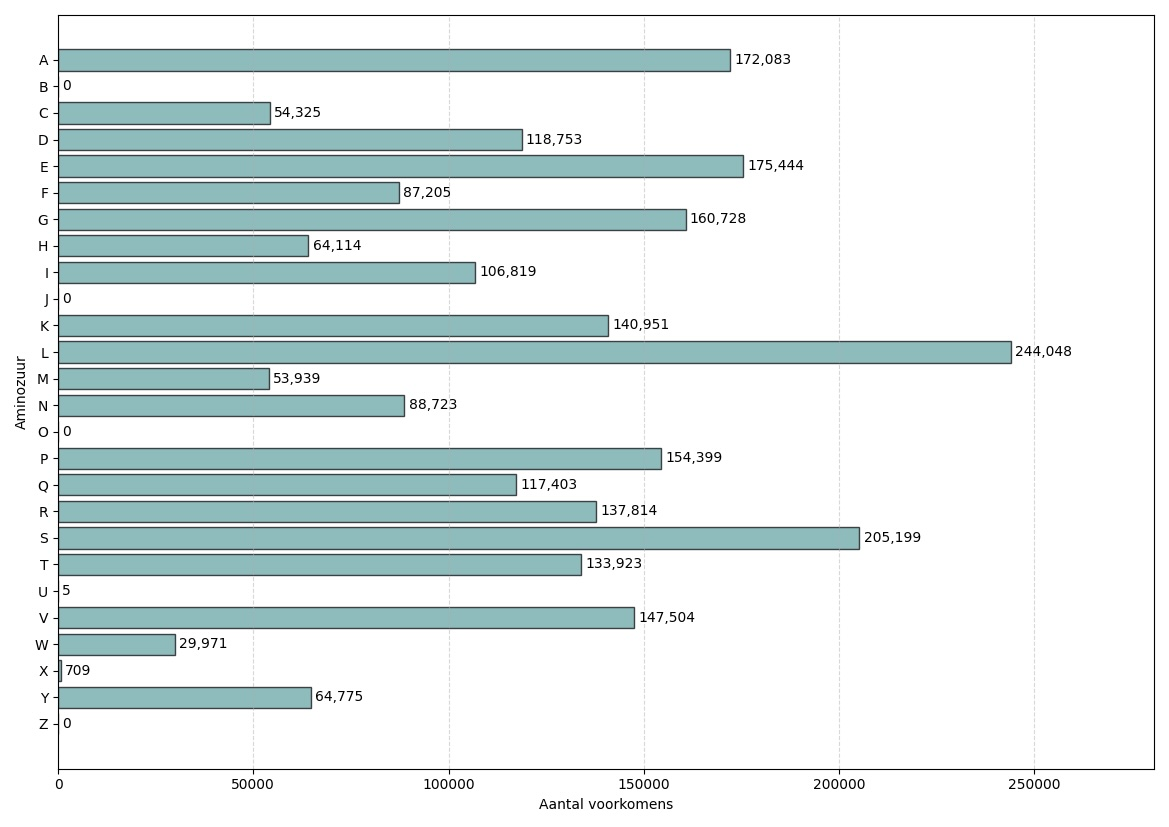
\includegraphics[width=0.90\linewidth]{humanprot_search_amino_acids}
    \caption{Distributie van de aminozuren in het Human-Prot peptidebestand.}
    \label{fig:humanprot_search_amino_acids}
\end{figure}

\begin{figure}[H]
    \centering
    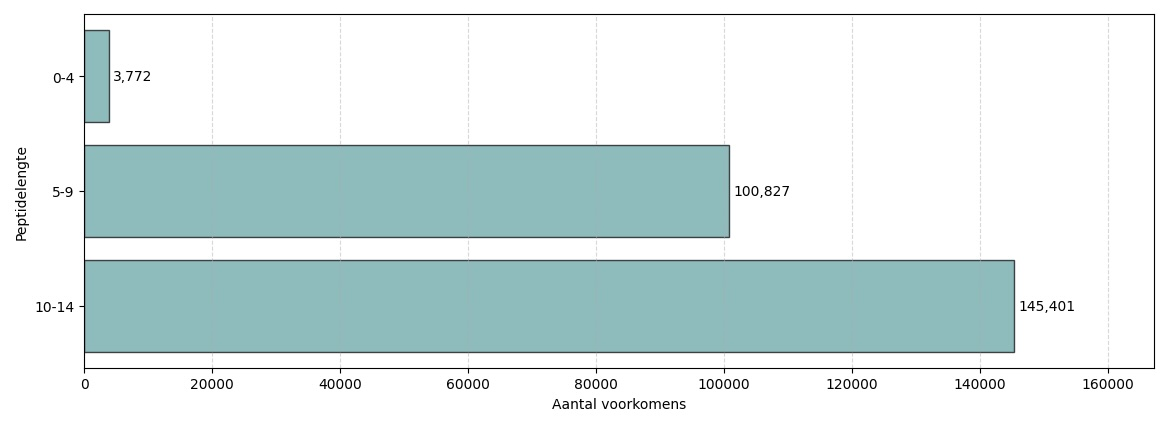
\includegraphics[width=0.90\linewidth]{humanprot_search_lengths}
    \caption{Lengtedistributie van de peptiden in het Human-Prot peptidebestand.}
    \label{fig:humanprot_search_distr}
\end{figure}

\section{Swiss-Prot}\label{sec:swiss-prot-stats}
\begin{figure}[H]
    \centering
    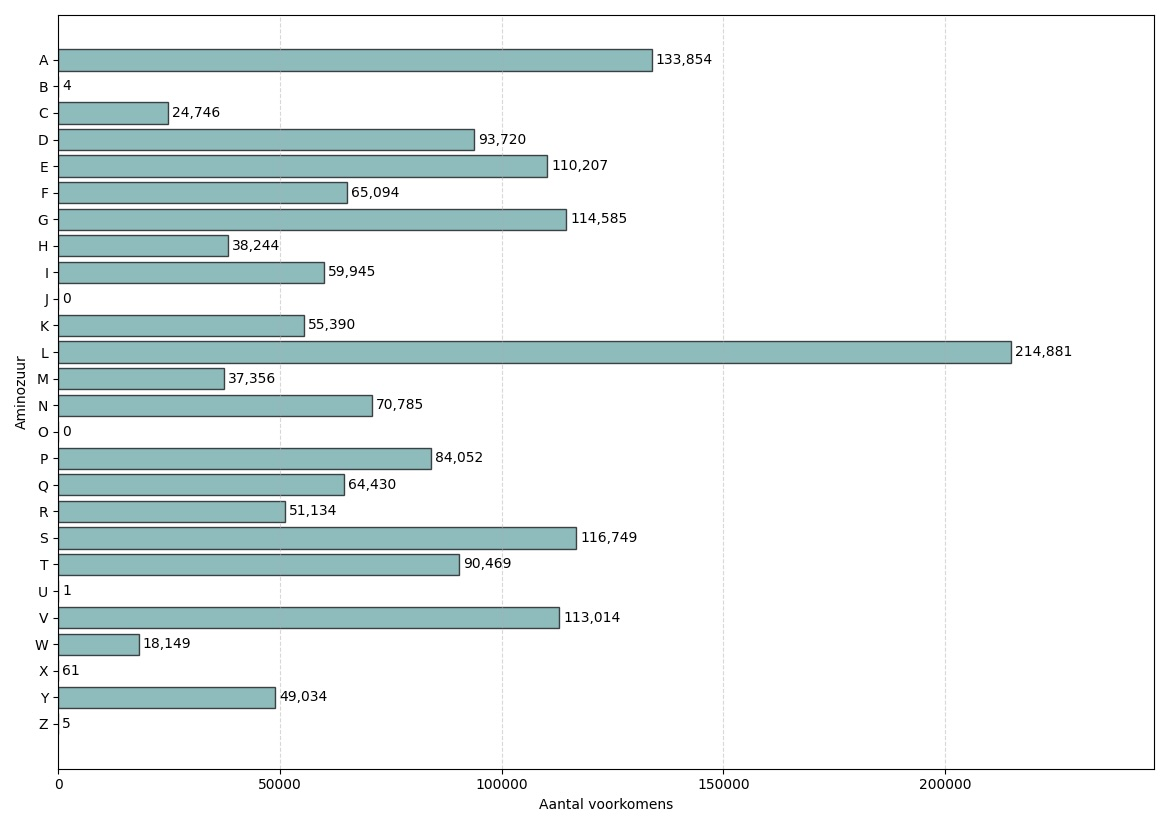
\includegraphics[width=0.90\linewidth]{swissprot_searchfile_no_missed_cleavage_amino_acids}
    \caption{Distributie van de aminozuren in het Swiss-Prot peptidebestand zonder \textit{missed cleavage.}}
    \label{fig:swissprot_search_no_missed_cleavage_amino_acids}
\end{figure}

\begin{figure}[H]
    \centering
    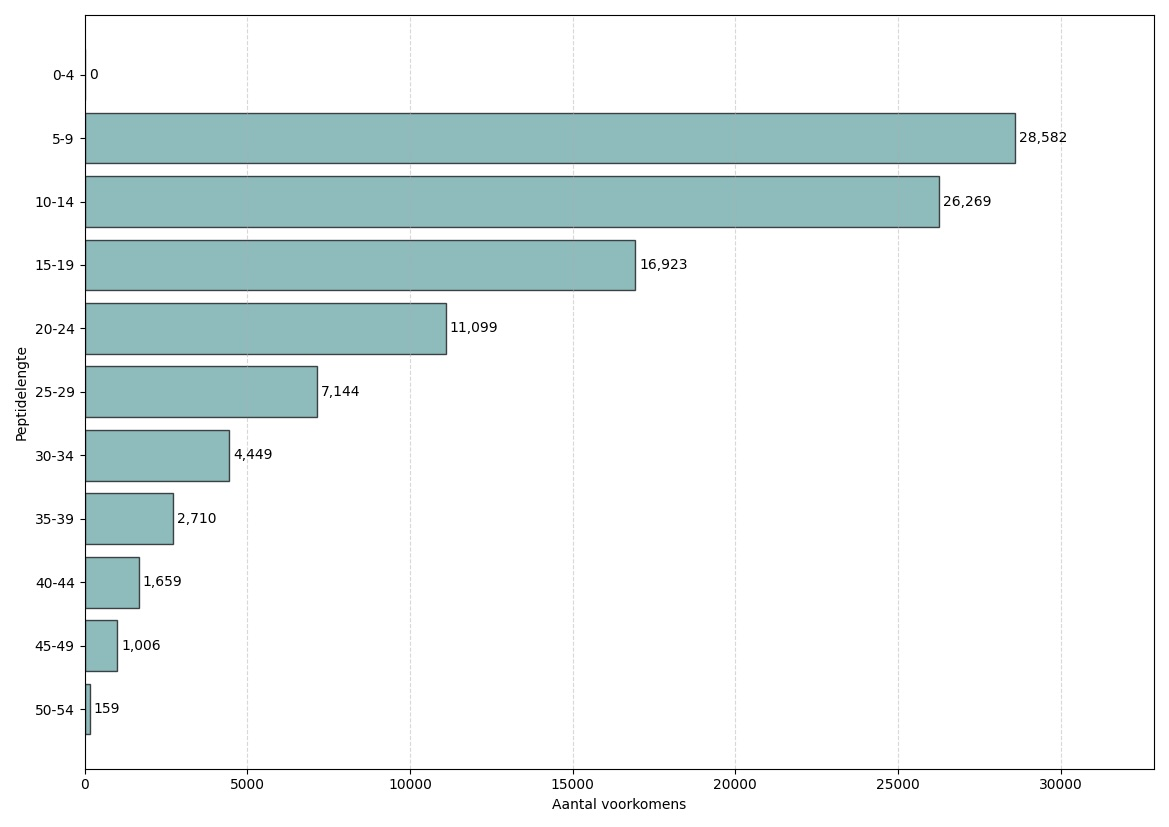
\includegraphics[width=0.90\linewidth]{swissprot_searchfile_no_missed_cleavage_lengths}
    \caption{Lengtedistributie van de peptiden in het Swiss-Prot peptidebestand zonder \textit{missed cleavage.}}
    \label{fig:swissprot_search_no_missed_cleavage_distr}
\end{figure}

\begin{figure}[H]
    \centering
    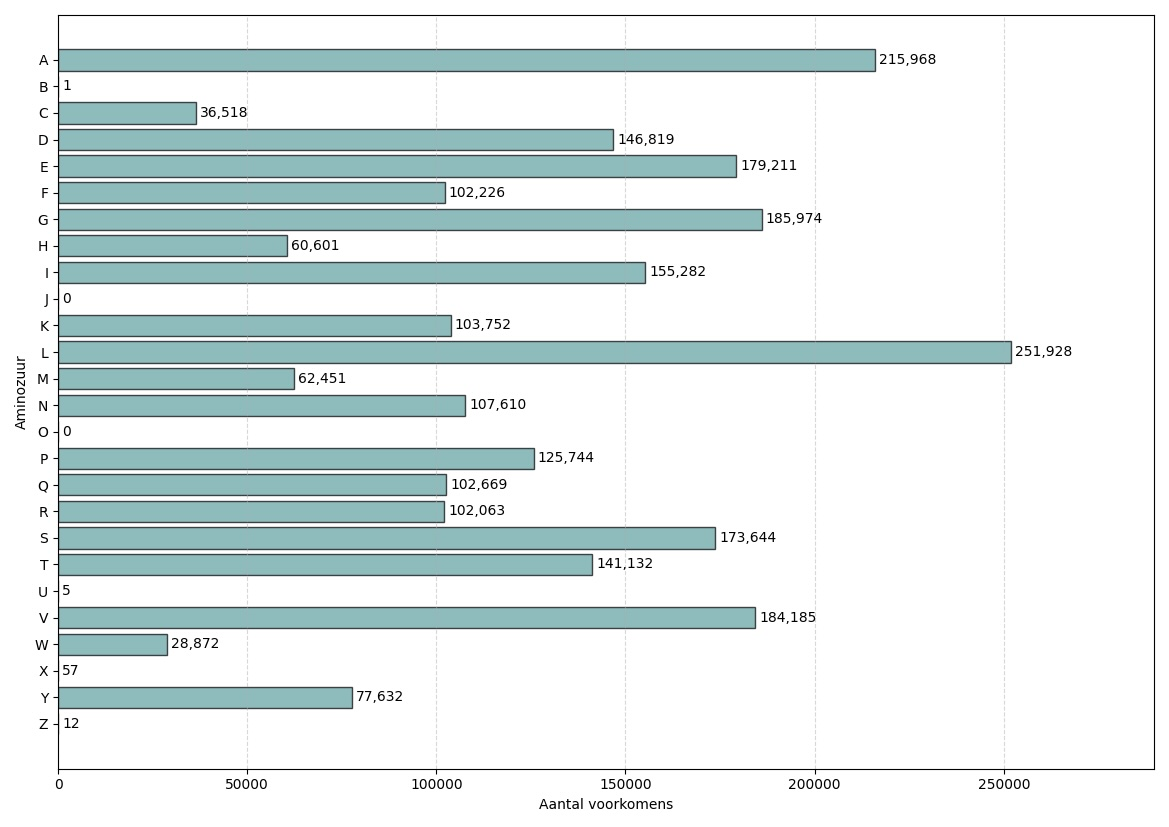
\includegraphics[width=0.90\linewidth]{swissprot_searchfile_missed_cleavage_amino_acids}
    \caption{Distributie van de aminozuren in het Swiss-Prot peptidebestand met \textit{missed cleavage.}}
    \label{fig:swissprot_search_missed_cleavage_amino_acids}
\end{figure}

\begin{figure}[H]
    \centering
    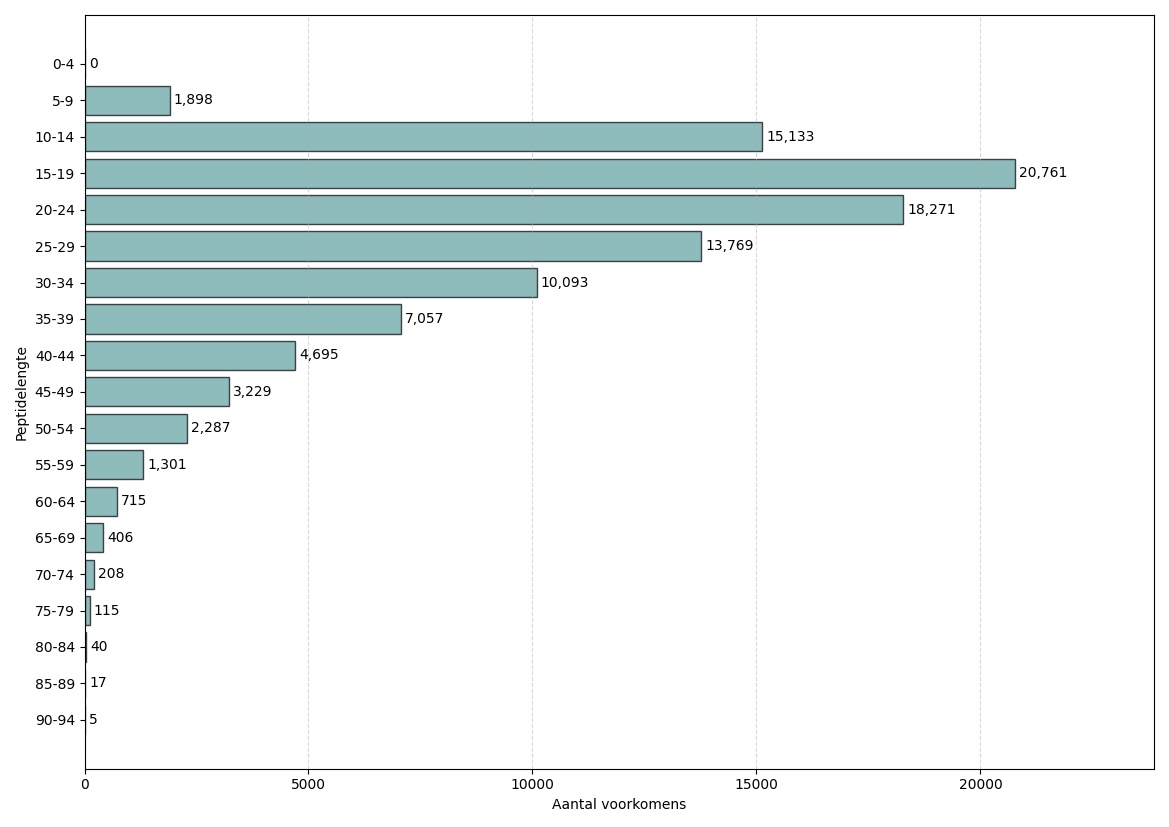
\includegraphics[width=0.90\linewidth]{swissprot_searchfile_missed_cleavage_lengths}
    \caption{Lengtedistributie van de peptiden in het Swiss-Prot peptidebestand met \textit{missed cleavage.}}
    \label{fig:swissprot_search_missed_cleavage_distr}
\end{figure}

\section{SIHUMI}\label{sec:sihumi-stats}

\begin{figure}[H]
    \centering
    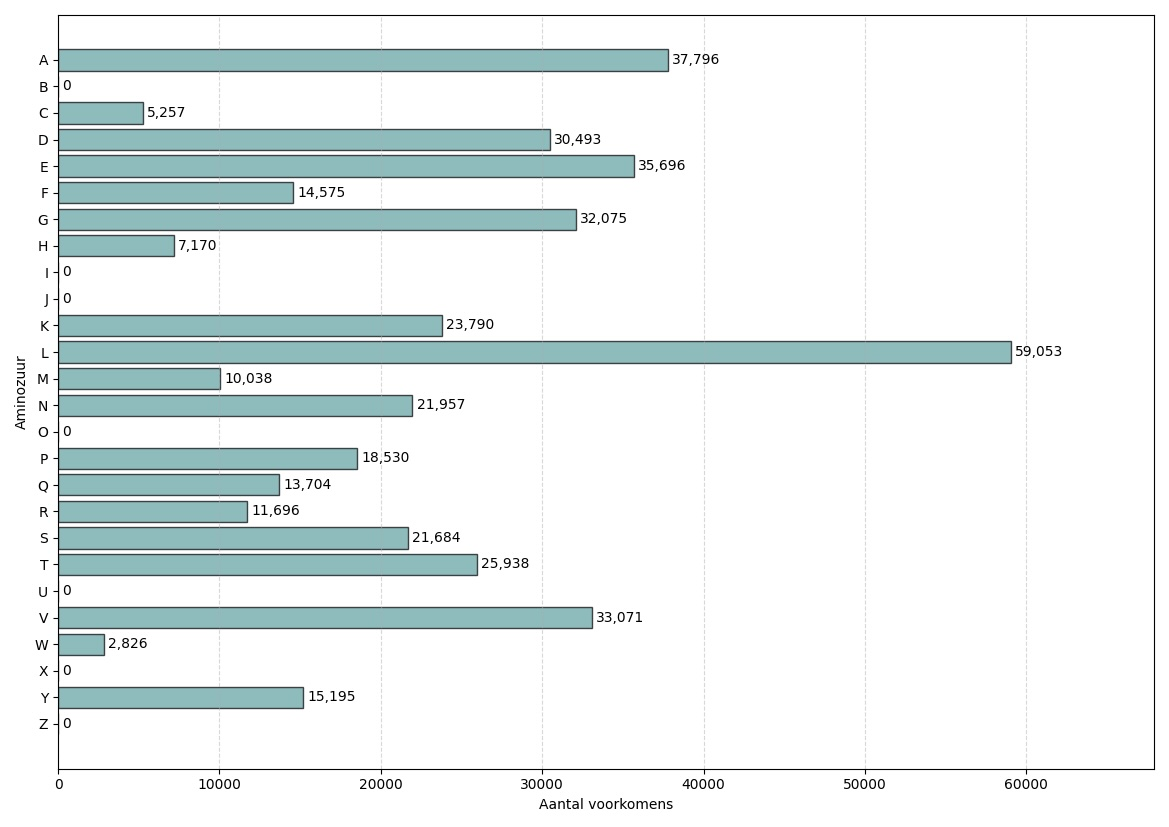
\includegraphics[width=0.90\linewidth]{sihumi_03_amino_acids}
    \caption{Distributie van de aminozuren in het SIHUMI 03 peptidebestand.}
    \label{fig:sihumi_03_amino_acids}
\end{figure}

\begin{figure}[H]
    \centering
    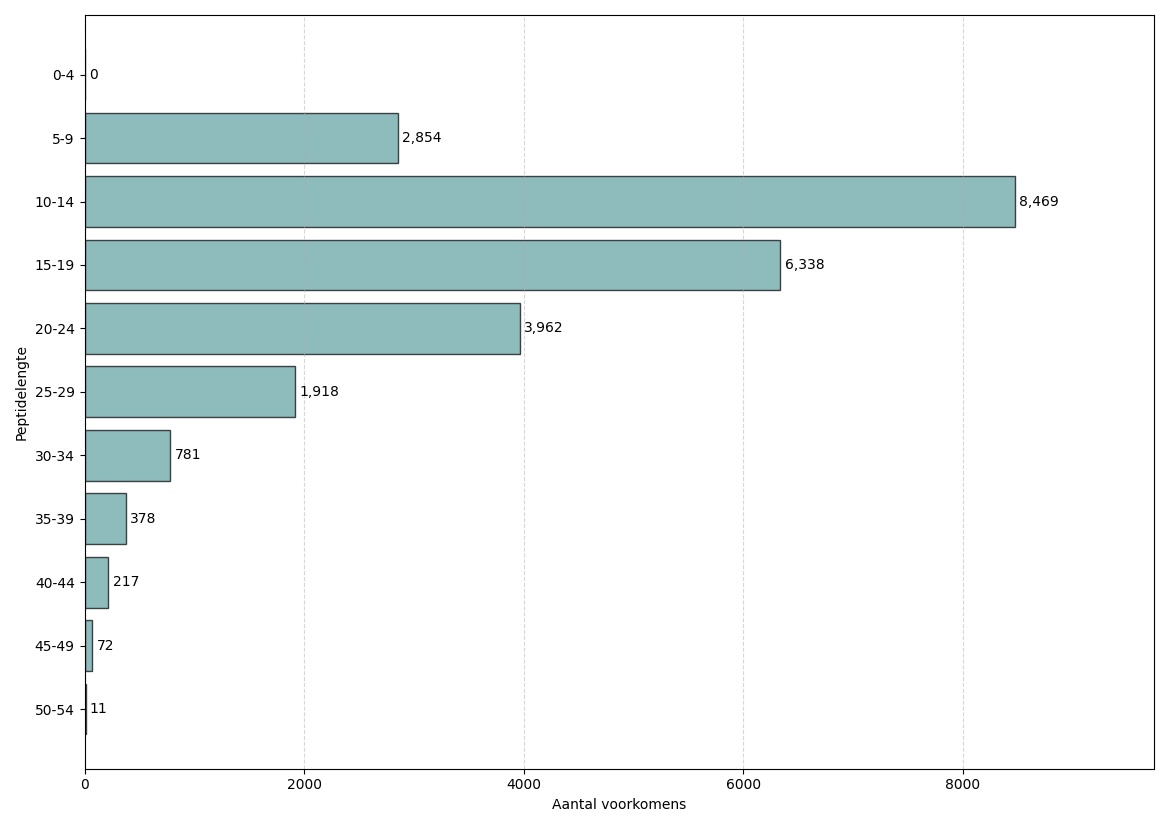
\includegraphics[width=0.90\linewidth]{sihumi_03_length}
    \caption{Lengtedistributie van de peptiden in het in het SIHUMI 03 peptidebestand.}
    \label{fig:sihumi_03_distr}
\end{figure}

\begin{figure}[H]
    \centering
    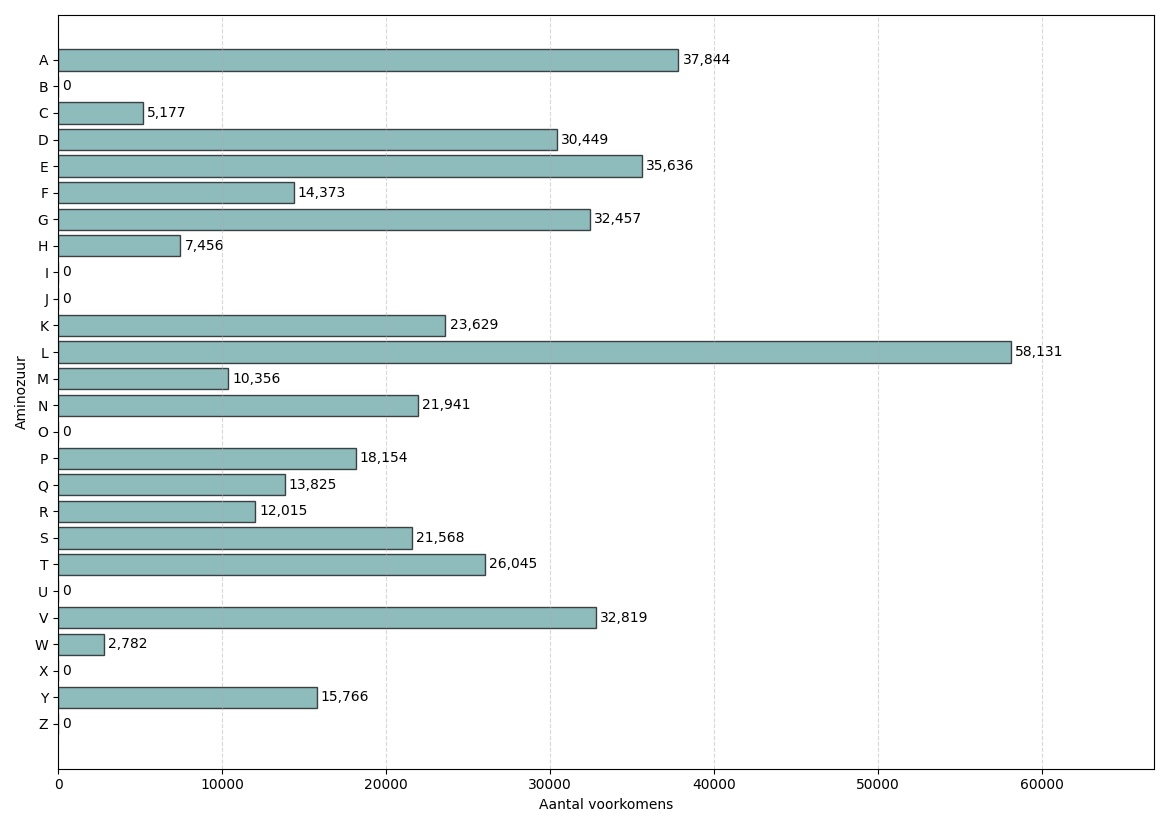
\includegraphics[width=0.90\linewidth]{sihumi_05_amino_acids}
    \caption{Distributie van de aminozuren in het SIHUMI 05 peptidebestand.}
    \label{fig:sihumi_05_amino_acids}
\end{figure}

\begin{figure}[H]
    \centering
    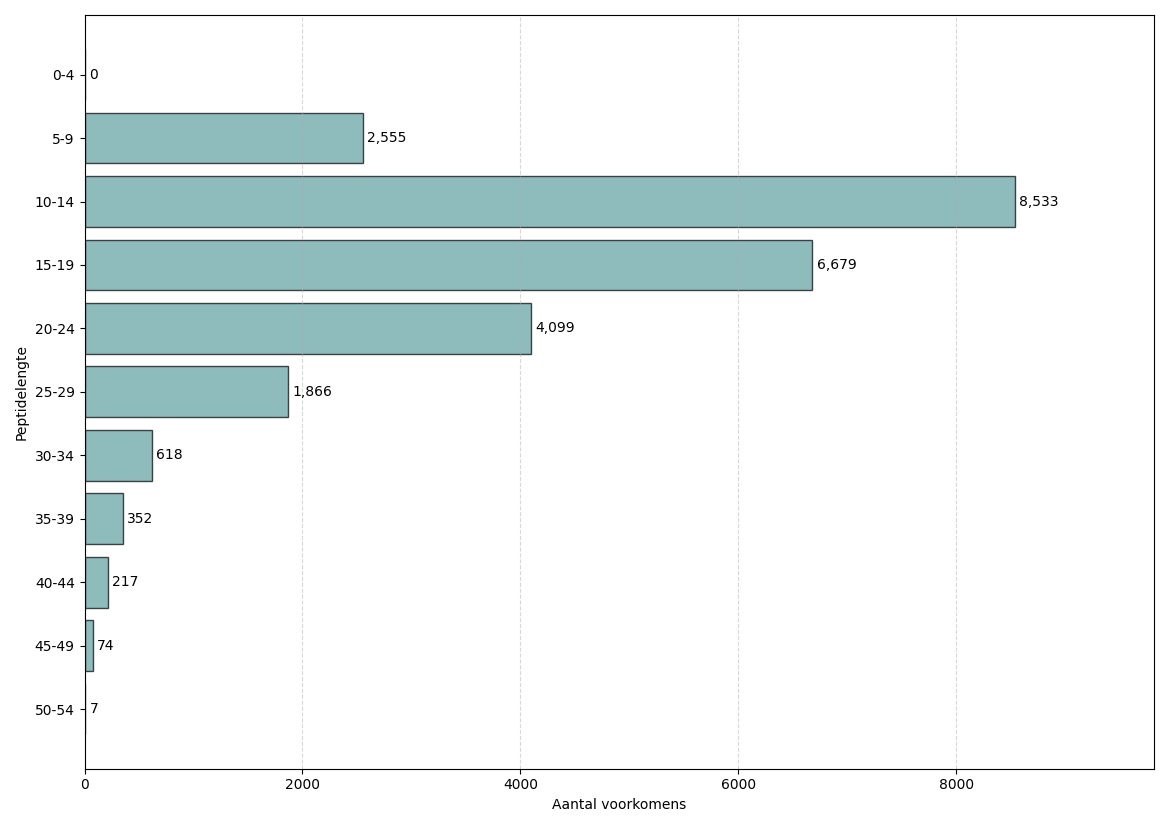
\includegraphics[width=0.90\linewidth]{sihumi_05_length}
    \caption{Lengtedistributie van de peptiden in het in het SIHUMI 05 peptidebestand.}
    \label{fig:sihumi_05_distr}
\end{figure}

\begin{figure}[H]
    \centering
    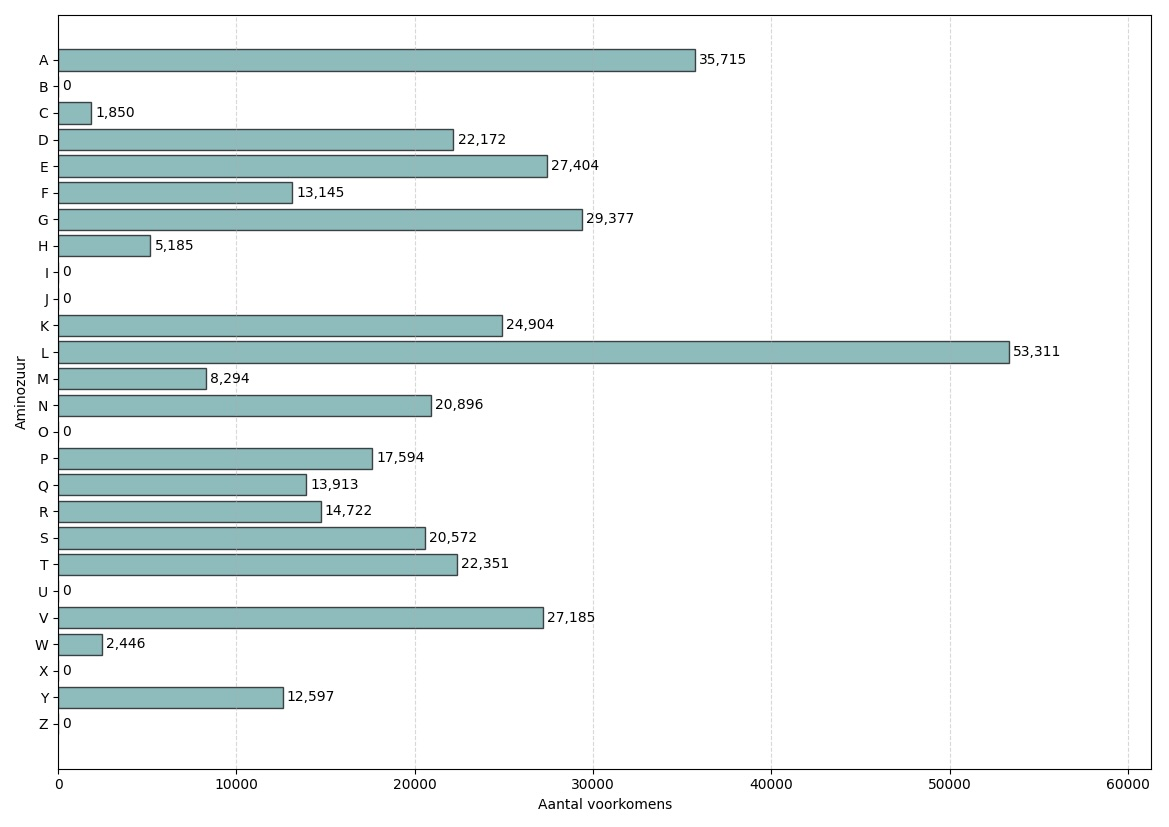
\includegraphics[width=0.90\linewidth]{sihumi_07_amino_acids}
    \caption{Distributie van de aminozuren in het SIHUMI 07 peptidebestand.}
    \label{fig:sihumi_07_amino_acids}
\end{figure}

\begin{figure}[H]
    \centering
    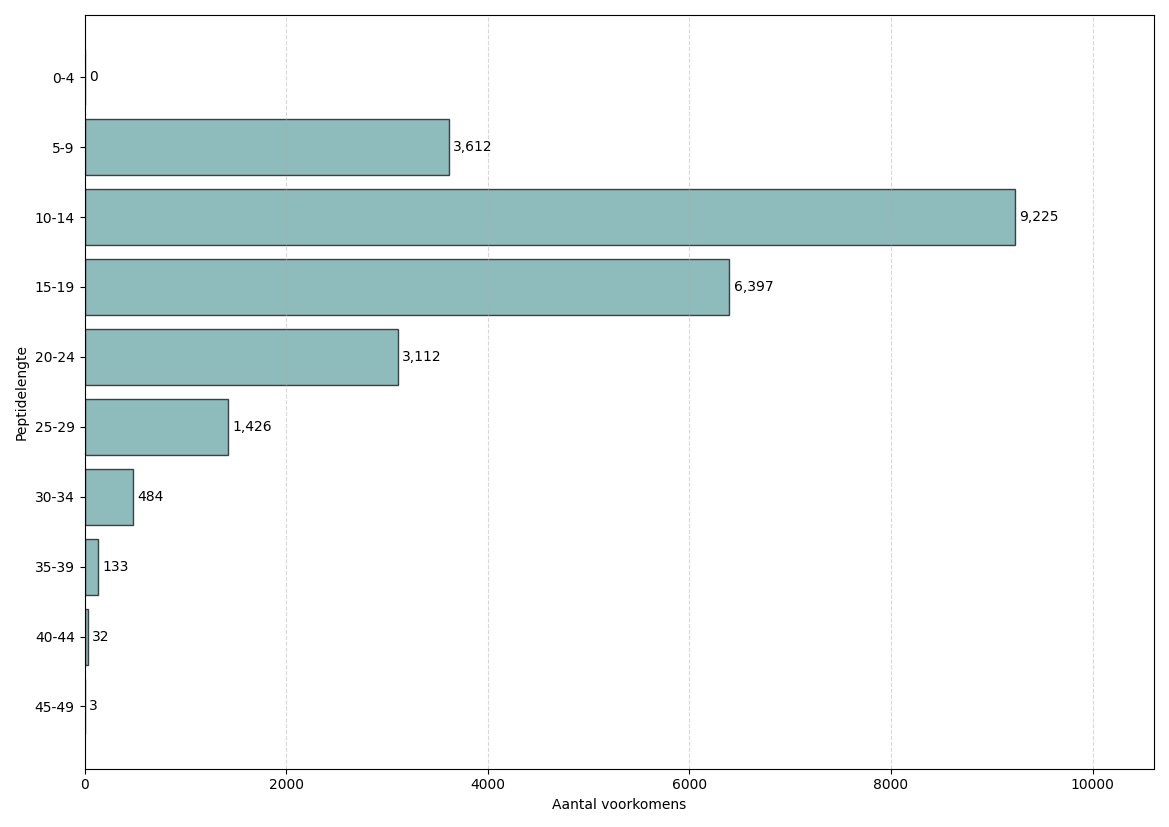
\includegraphics[width=0.90\linewidth]{sihumi_07_length}
    \caption{Lengtedistributie van de peptiden in het in het SIHUMI 07 peptidebestand.}
    \label{fig:sihumi_07_distr}
\end{figure}

\begin{figure}[H]
    \centering
    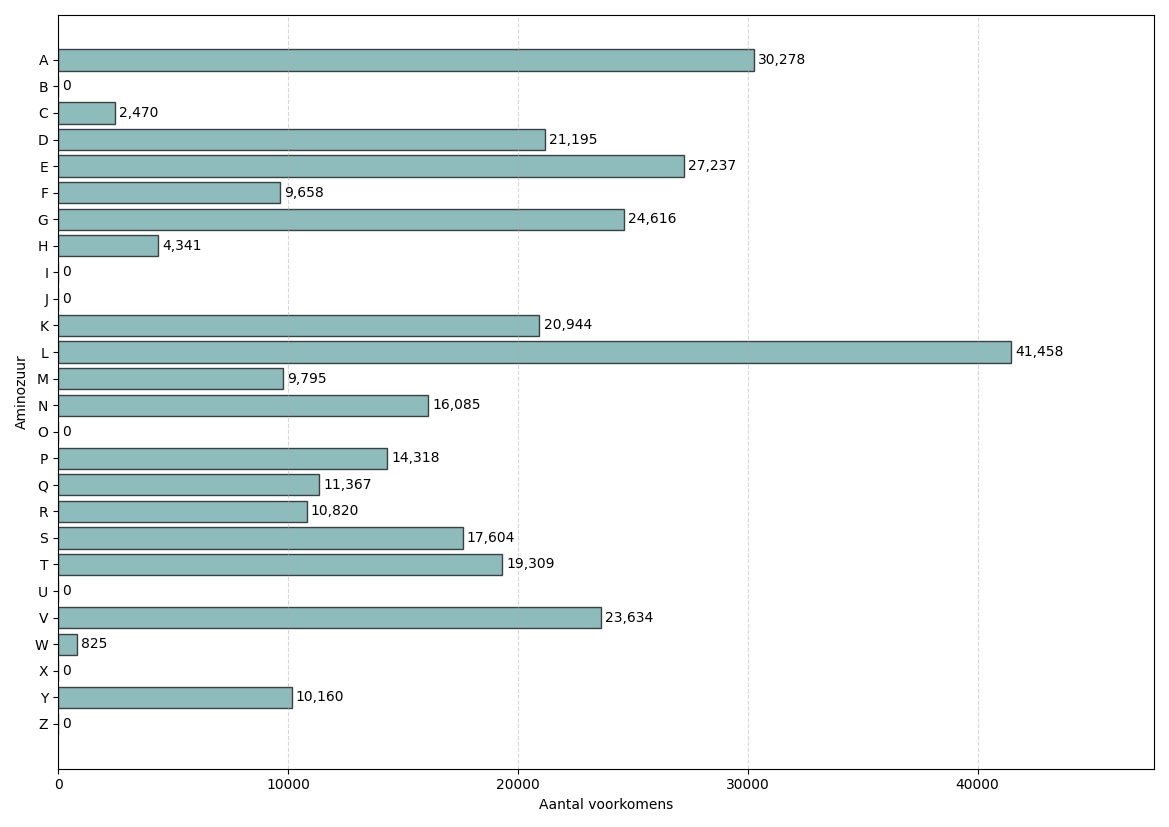
\includegraphics[width=0.90\linewidth]{sihumi_08_amino_acids}
    \caption{Distributie van de aminozuren in het SIHUMI 08 peptidebestand.}
    \label{fig:sihumi_08_amino_acids}
\end{figure}

\begin{figure}[H]
    \centering
    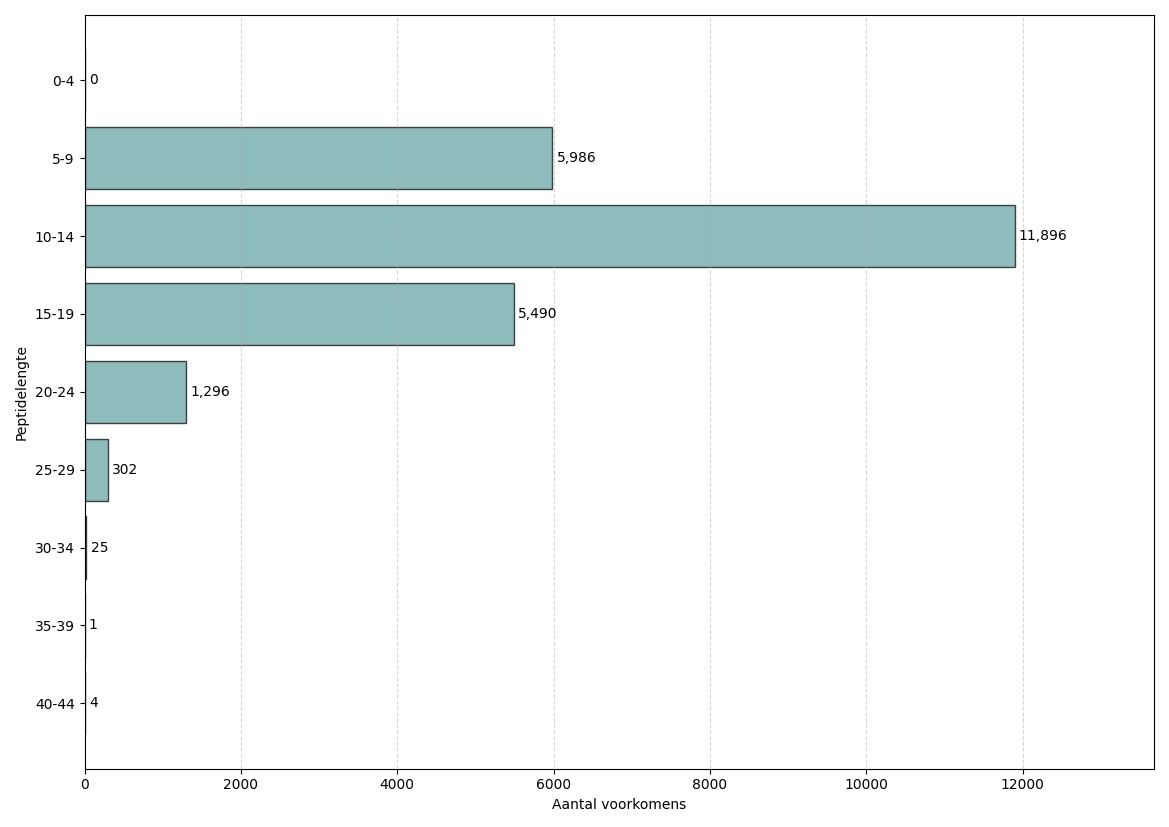
\includegraphics[width=0.90\linewidth]{sihumi_08_length}
    \caption{Lengtedistributie van de peptiden in het in het SIHUMI 08 peptidebestand.}
    \label{fig:sihumi_08_distr}
\end{figure}

\begin{figure}[H]
    \centering
    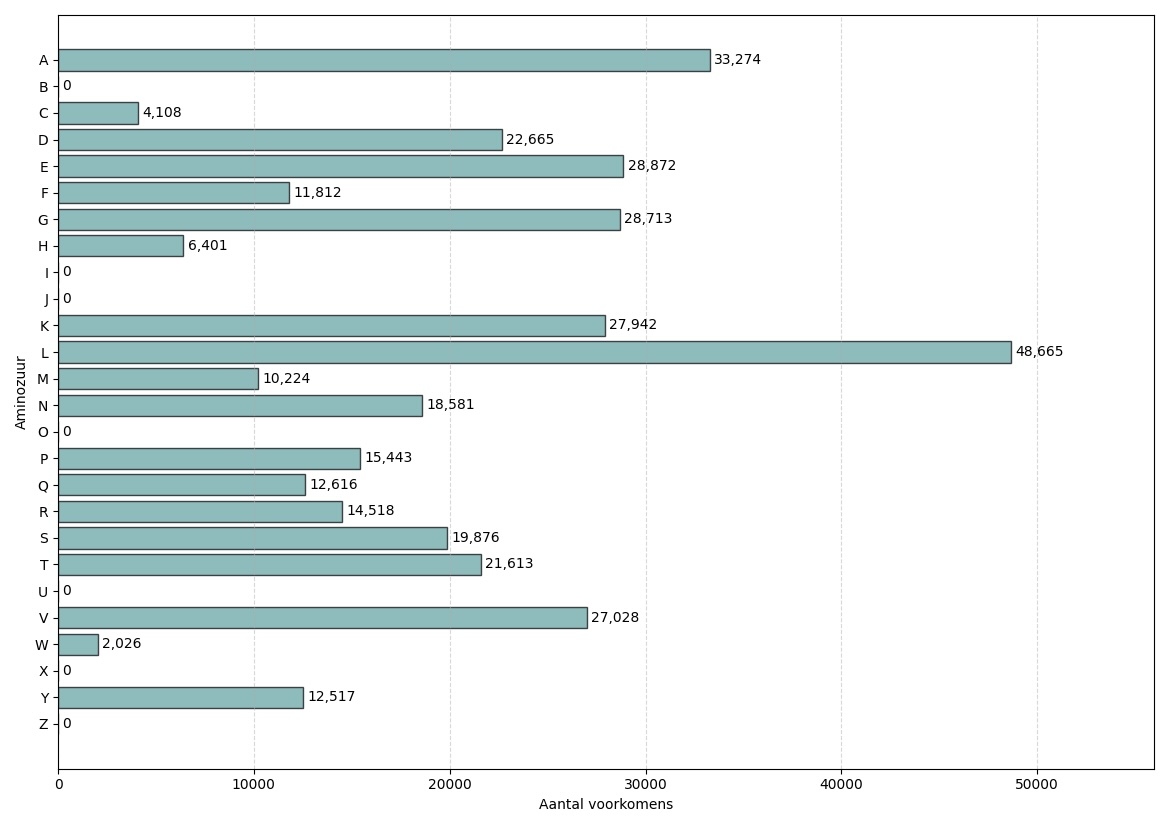
\includegraphics[width=0.90\linewidth]{sihumi_11_amino_acids}
    \caption{Distributie van de aminozuren in het SIHUMI 11 peptidebestand.}
    \label{fig:sihumi_11_amino_acids}
\end{figure}

\begin{figure}[H]
    \centering
    \includegraphics[width=0.90\linewidth]{sihumi_11_length}
    \caption{Lengtedistributie van de peptiden in het in het SIHUMI 11 peptidebestand.}
    \label{fig:sihumi_11_distr}
\end{figure}

\begin{figure}[H]
    \centering
    \includegraphics[width=0.90\linewidth]{sihumi_14_amino_acids}
    \caption{Distributie van de aminozuren in het SIHUMI 14 peptidebestand.}
    \label{fig:sihumi_14_amino_acids}
\end{figure}

\begin{figure}[H]
    \centering
    \includegraphics[width=0.90\linewidth]{sihumi_14_length}
    \caption{Lengtedistributie van de peptiden in het in het SIHUMI 14 peptidebestand.}
    \label{fig:sihumi_14_distr}
\end{figure}
    \chapter{Unipept protein counts distribution}\label{ch:appendix-unipept-protein-counts-distribution}
\begin{table}[h!]
    \centering
    \begin{tabular}{|l|r|}
        \hline
        \textbf{\# Proteïnes} & \textbf{\# Peptiden}\\
        \hline
        $\geq 1$     & 1\thinspace342\thinspace470\thinspace764 \\
        $\geq 2$     & 355\thinspace979\thinspace324            \\
        $\geq 10$    & 38\thinspace697\thinspace210             \\
        $\geq 10^2$  & 2\thinspace921\thinspace879              \\
        $\geq 10^3$  & 217\thinspace922                         \\
        $\geq 10^4$  & 13\thinspace008                          \\
        $\geq 10^5$  & 118                                      \\
        $\geq 10^6$  & 0                                        \\ \hline
    \end{tabular}
    \caption{Het aantal verschillende tryptische peptiden die matchen met op zijn minst $x$ proteïnes uit UniProtKB 2023\_03. Een klein voorbeeld: stel dat we de tryptiche peptide \texttt{ACACA} zoeken. Deze heeft 24\thinspace694 matches in UniProtKB. Dit wil zeggen dat dit één van de 13\thinspace008 peptiden is met meer dan $10^4$ matches.}
    \label{tab:number_peptide_matches}
\end{table}

\begin{table}[h!]
    \centering
    \begin{tabular}{|l|r|}
        \hline
        \textbf{\# NCBI taxonomy rank} & \textbf{\# Peptiden} \\ \hline
        root & 12\thinspace369 \\ \hline
        superkingdom & 43 \\ \hline
        kingdom & 16 \\ \hline
        subkingdom & 0 \\ \hline
        superphylum & 0 \\ \hline
        phylum & 8 \\ \hline
        subphylum & 7 \\ \hline
        superclass & 1 \\ \hline
        class & 18 \\ \hline
        subclass & 1 \\ \hline
        superorder & 0 \\ \hline
        order & 0 \\ \hline
        infraorder & 1 \\ \hline
        superfamily & 0 \\ \hline
        family & 2 \\ \hline
        subfamily & 0 \\ \hline
        tribe & 1 \\ \hline
        subtribe & 0 \\ \hline
        genus & 55 \\ \hline
        subgenus & 0 \\ \hline
        species\_group & 0 \\ \hline
        species\_subgroup & 0 \\ \hline
        species & 200 \\ \hline
        subspecies & 0 \\ \hline
        strain & 1 \\ \hline
        varietas & 0 \\ \hline
        forma & 0 \\ \hline
    \end{tabular}
    \caption{Verdeling van de 13\thinspace000 verschillende peptiden die met meer $\geq 10^4$ proteïnes matchen. We zien dat voor de overgrote meerderheid de LCA resulteert op de root. Slechts voor 200 peptiden is het resultaat op soortniveau.}
    \label{tab:peptides_distribution}
\end{table}

\begin{table}[h!]
    \centering
    \begin{tabular}{|r|l|}
        \hline
        \textbf{\# Peptiden} & \textbf{LCA} \\ \hline
        119 & \textit{Alphainfluenzavirus influenzae} \\ \hline
        32 & \textit{Human immunodeficiency virus} \\ \hline
        14 & \textit{Hepatitis B virus} \\ \hline
        9 & \textit{Betainfluenzavirus influenzae} \\ \hline
        4 & \textit{Orthoflavivirus denguei} \\ \hline
        3 & \textit{Simian immunodeficiency virus}   \\ \hline
        1 & \textit{Alcidodes juglans} \\ \hline
        1 & \textit{Bacillus subtilis} \\ \hline
        1 & \textit{Bacteroides thetaiotaomicron} \\ \hline
        1 & \textit{Cannabis sativa} \\ \hline
        1 & \textit{Capsicum baccatum} \\ \hline
        1 & \textit{Echinocucumis hispida} \\ \hline
        1 & \textit{Geissoloma marginatum} \\ \hline
        1 & \textit{Homo sapiens} \\ \hline
        1 & \textit{Human immunodeficiency virus} \\ \hline
        1 & \textit{Kalanchoe fedtschenkoi} \\ \hline
        1 & \textit{Leucosceptrum canum} \\ \hline
        1 & \textit{Loxia curvirostra} \\ \hline
        1 & \textit{Marinilactibacillus piezotolerans} \\ \hline
        1 & \textit{Melanocenchris jacquemontii} \\ \hline
        1 & \textit{Merops nubicus} \\ \hline
        1 & \textit{Morbillivirus hominis} \\ \hline
        1 & \textit{Phalaenopsis pulcherrima} \\ \hline
        1 & \textit{Phormidesmis priestleyi} \\ \hline
        1 & \textit{Rhodobacter maris} \\ \hline
    \end{tabular}
    \caption{Overzicht van de geassocieerde soort voor de 200 peptiden uit tabel~\ref{tab:peptides_distribution} die op soortniveau eindigen.
    Van de 200 peptiden eindigt de meerderheid in een LCA die geassocieerd is met een virus (zoals HIV of influenza). Dit komt doordat er veel onderzoek gedaan wordt naar de verschillende bestaande rassen. Deze zitten allemaal in de UniProt Knowledgebase.}
    \label{tab:peptides_species}
\end{table}


\end{document}